\documentclass[20pt]{beamer}
%\usepackage[size=a4]{beamerposter}
\usepackage{graphicx} % Required for inserting images
\usepackage[utf8]{inputenc}
\geometry{showframe,paperwidth=210mm,paperheight=297mm}
\setbeamertemplate{caption}[numbered]
\numberwithin{figure}{section}


%\setbeamerfont{frametitle}{size = \LARGE}


\usetheme{Madrid}
\usecolortheme{seahorse}



\logo{
\includegraphics[height=2cm]{logo.png}}

\usepackage{tikz}
\usepackage{hyperref}
\usepackage{xcolor}
\usepackage{algpseudocode}
\usepackage{algorithm}
\usepackage{fancyvrb}
\usepackage{ragged2e}
\usepackage{multicol}

\usetikzlibrary{shapes.geometric, arrows}




%\setbeamercolor{itemize item}{fg=red}
%\setbeamercolor{block body}{bg=white}
%\setbeamercolor{block title}{bg=orange!50, fg=black}
%\addbibresource{Bibliographies/EK_.bib}

\title{Lab Inventory Management System}
\author[Group : 3 || Subsection : B2]{
    \begin{tabular}{|c|c|}
        \hline
        1905091 & Sadia Tabassum \\
        \hline
        1905099 & Alina Zaman \\
        \hline
        1905102 & Md. Shafiul Haque \\
        \hline
        1905103 & Mayesha Rashid \\
        \hline
        1905104 & Kazi Istiak Toriqe \\
        \hline
        1905119 & Saha Kuljit Shantanu \\    
        \hline
    \end{tabular}
}

\institute[]{

    Course : CSE 326(Information System Design Sessional)
    \\
    \vspace{10}
    \textcolor{black!60}{DEPARTMENT OF COMPUTER SCIENCE AND ENGINEERING, }
    \\ 
    \vspace{10}
    \textcolor{black!60}{BANGLADESH UNIVERSITY OF ENGINEERING AND TECHNOLOGY}
}
\date{September 2023}



\begin{document}

\frame{\titlepage}

%\usebackgroundtemplate{}

\begin{frame}{Table of Contents}

\tableofcontents
    
\end{frame}

\AtBeginSection[]{
  \begin{frame}
  \frametitle{Discussion Topic}
  \tableofcontents[currentsection,currentsubsection]
  \end{frame}
}

\section{Overview of the project}

\begin{frame}{Overview Of the Project}



  \begin{alertblock}{Aim}
         
     

    \vspace{10}

    \justifying{The project is to look into the inventory management system of the laboratories of our institute and implement it in a more sophisticated way for the laboratory users, be it students , laboratory assistants or teachers, to use more conveniently.}

    \vspace{10}

  \end{alertblock}

  \vspace{80}

  \begin{exampl4eblock}{Motivation}

    \vspace{10} 
     \justifying{The motivation is that there are sufficient scope to improvise the existing laboratory management system of our institute. The suitable ideas and efforts that will make this project successful will be taken into account}

    \vspace{10}

  \end{exampleblock}

\end{frame}


\section{Corrections made to the project}

\begin{frame}

\frametitle{Corrections made to the project}

\begin{thebibliography}{99}

\bibitem{my_label}
\textbf{\footnotesize{Error and Corrections to BPMN}} 

\href{https://github.com/Saha-Kuljit-Shantanu/CSE_326_INFORMATION_SYSTEM_DESIGN_SESSIONAL/blob/main/BPMN_DIAGRAM_ERRORS_AND_CORRECTIONS.md}{\underline{\footnotesize{Click here}}}

\vspace{15}

\bibitem{my_label}
\textbf{\footnotesize{Error and Corrections to ERD}} 

\href{https://github.com/Saha-Kuljit-Shantanu/CSE_326_INFORMATION_SYSTEM_DESIGN_SESSIONAL/blob/main/ER_DIAGRAM_ERRORS_AND_CORRECTIONS.md}{\underline{\footnotesize{Click here}}}

\vspace{15}

\bibitem{my_label}
\textbf{\footnotesize{Error and Corrections to Sequence Diagram}} 

\href{https://github.com/Saha-Kuljit-Shantanu/CSE_326_INFORMATION_SYSTEM_DESIGN_SESSIONAL/blob/main/SEQUENCE_DIAGRAM_ERRORS_AND_CORRECTIONS.md}{\underline{\footnotesize{Click here}}}

\vspace{15}

\end{thebibliography}

\end{frame}


\section{Business Process Model and Notation(BPMN)}

\begin{frame}{The Full BPMN Diagram}

     \begin{figure}
        \centering
        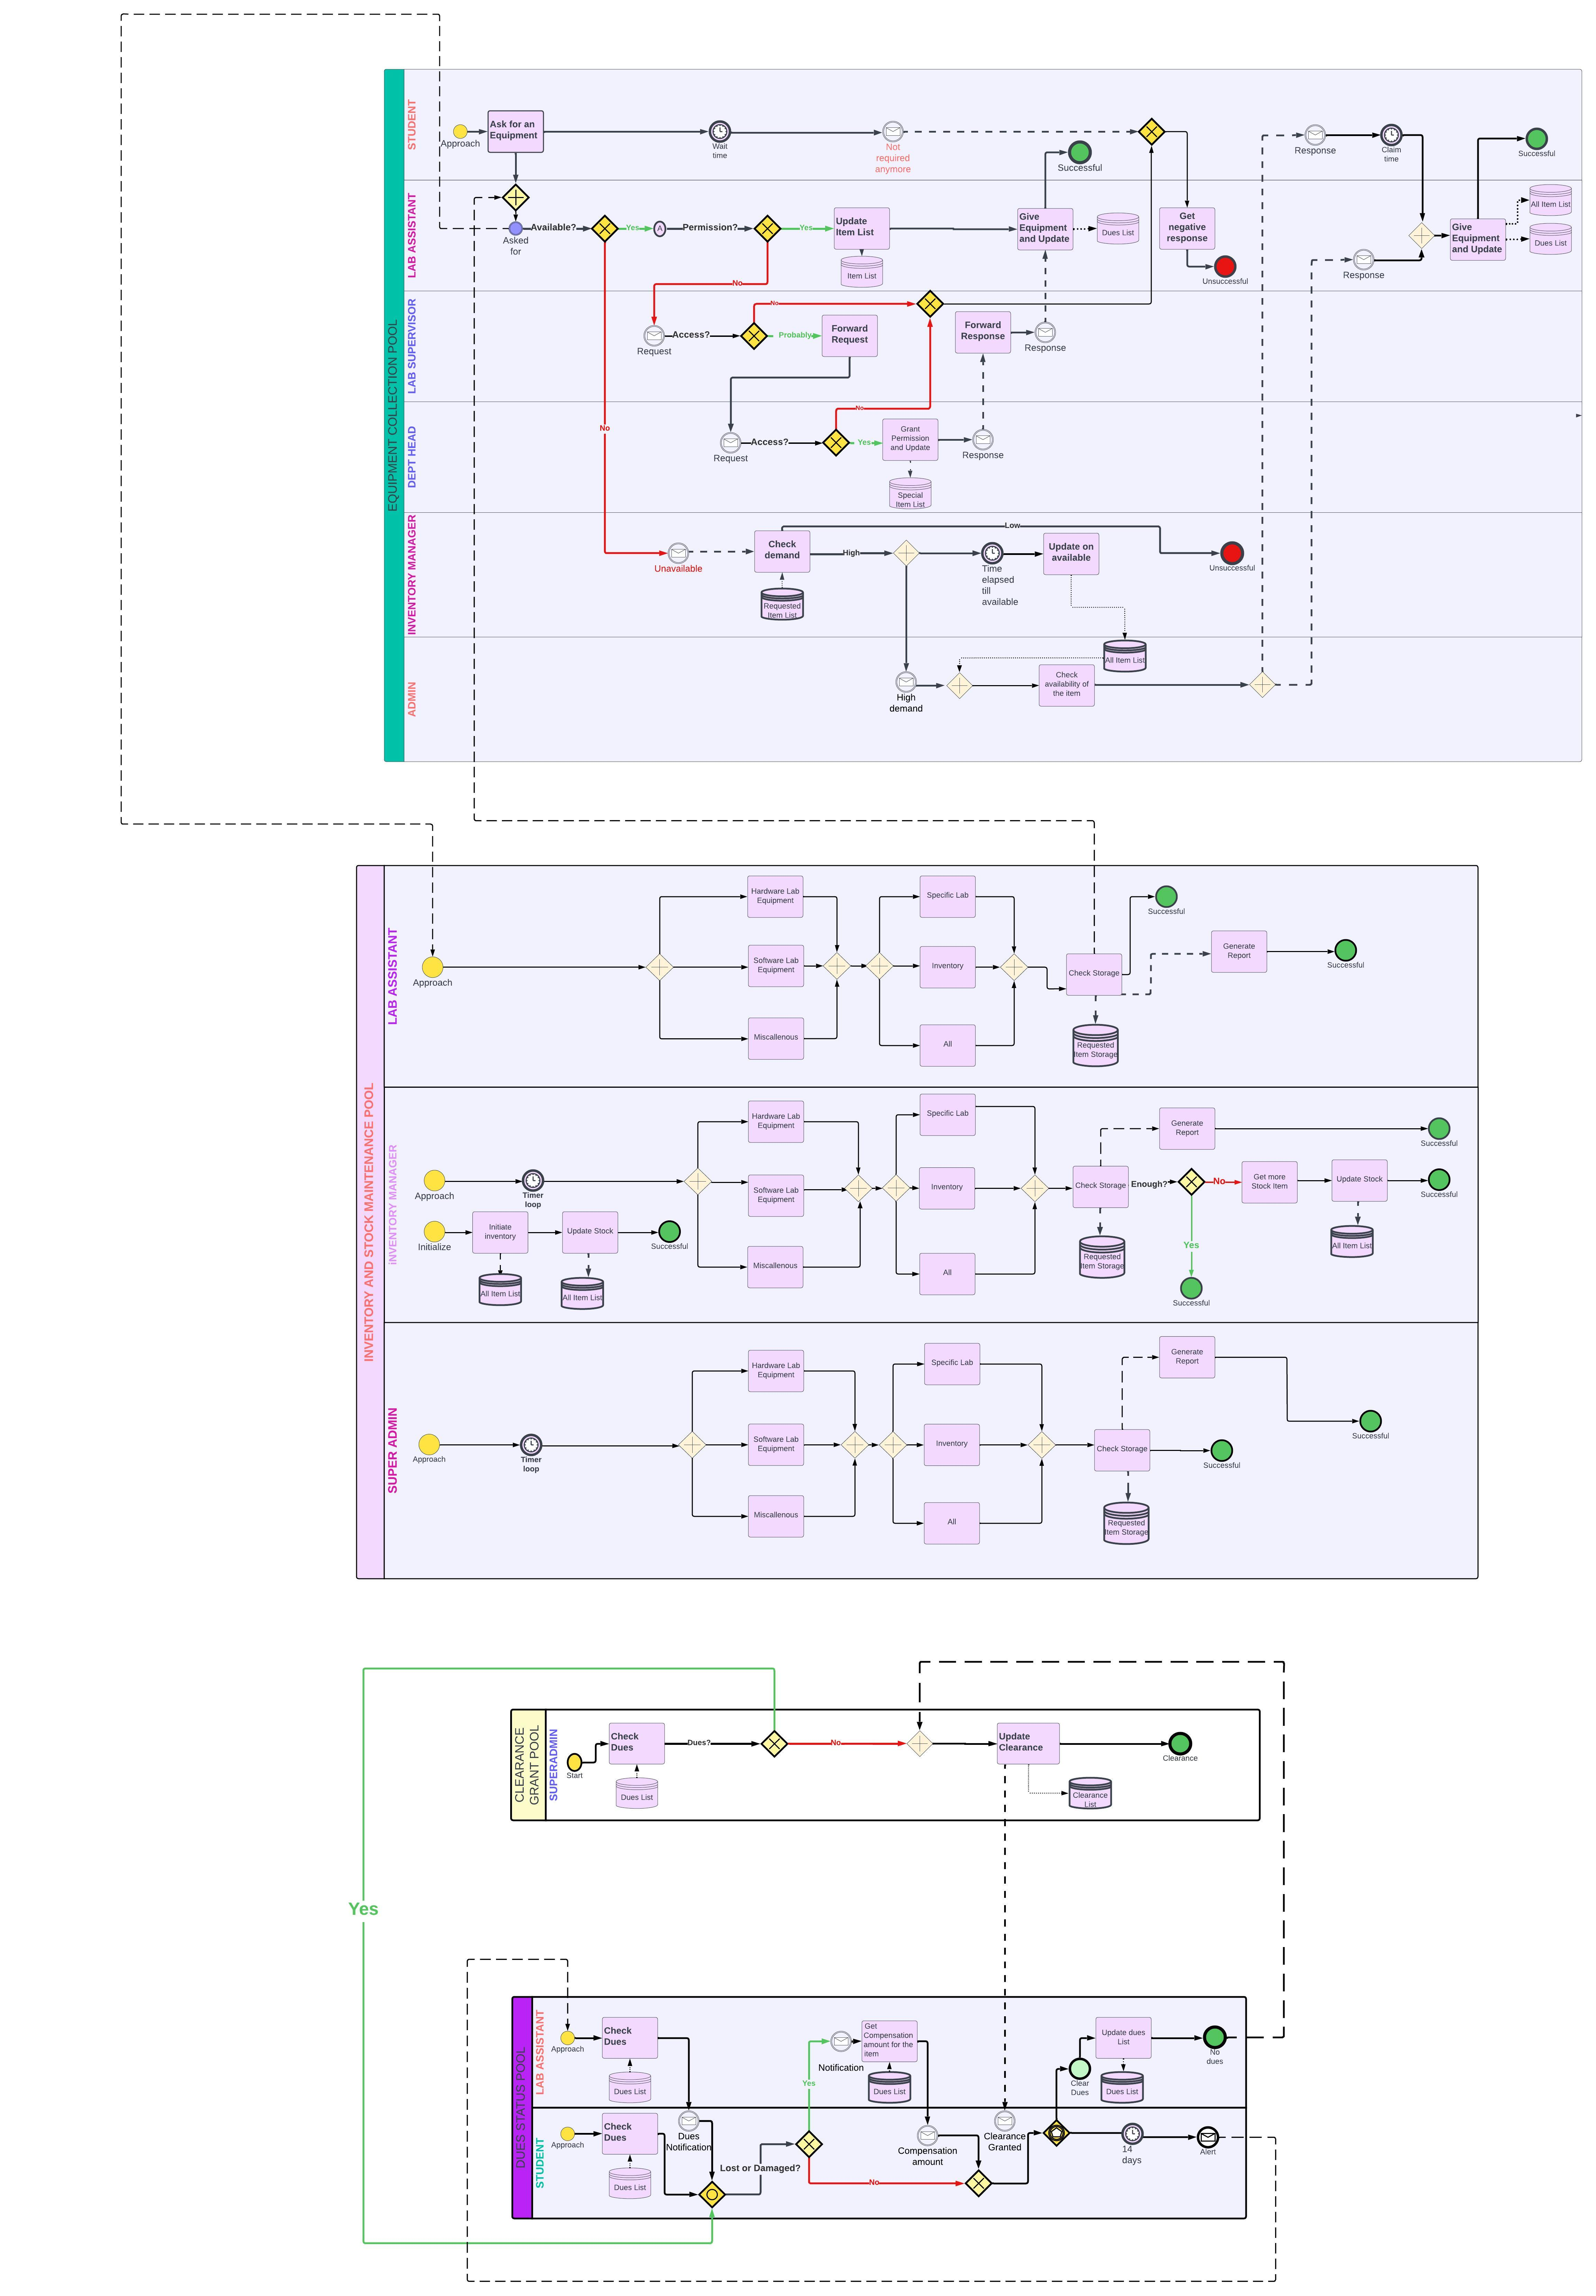
\includegraphics[width= 0.9\textwidth , height= 0.8\paperheight]{Full_BPMN.jpeg}
        \caption{{Full BPMN Diagram}}
        \label{fig:17}
    \end{figure}

\end{frame}

\begin{frame}{The Full BPMN Diagram}

    \begin{block}{Pools and Lanes of BPMN}

       \begin{itemize}

       \vspace{20}

       
        \item 
        \justifying{
        \textbf{Equipment Collection Pool: } This pool handles the process of requisition of stuff from inventory to students over an ongoing turn of events and might be unsuccessful in certain cases. The pool has 6 lanes :}\\
        \\

        \vspace{10}
        
        \begin{tabular}{ll}
           
        1) Student & 2) Lab Assistant  \\
        3) Lab Supervisor & 4) Department head\\
        5) Inventory Manager \hspace{40} & 6) Admin\\
        
        \end{tabular}
        
        \vspace{20}
            
        \item 
        \justifying{
        \textbf{Inventory and Stock Maintenance Pool: } This pool takes in account initialization of an inventory and handles the process of frequent checking and updating of stock based on recently occuring events, triggered unconditionally over a certain interval of time or conditionally for any requistion event. The pool has 3 lanes :}\\

        \vspace{10}
           
        1) Lab Assistant  \\
        2) Inventory Manager \\
        3) Super Admin\\
        \\

        \vspace{20}
        
        
        \end{itemize}
        
    \end{block}

\end{frame}

\begin{frame}{The Full BPMN Diagram}

    \begin{block}{Pools and Lanes of BPMN}

       \begin{itemize}

       \vspace{20}

        \item \justifying{
        \textbf{Dues Status Pool: } This pool deals with the process of not only checking out the dues of a student from the lab but also, in a case of losing or damaging any inventory goods, it keeps a track of the amount of money for compensation. For each due pointed by the lab assistant, the lab assistant is allowed to notify a student with the due in every 14 days until clearance. Having no dues is a successful state of this pool which opens a pathway to the clearance grant for a student. The pool has 2 lanes :}\\

        \vspace{10}
        
        \begin{tabular}{ll}
           
        1) Student \hspace{120} & 2) Lab Assistant  \\
        
        \end{tabular}
        
        \vspace{20}
        
        \item \justifying{
        \textbf{Clearance Grant Pool: } This pool handles the process of granting clearance to the student. If dues are found, it connects to the dues status pool. Only the superadmin can provide a clearance grant.}

        \vspace{20}

       \end{itemize}

    \end{block}

\end{frame}

\begin{frame}{Equipment Collection Pool}

    \begin{alertblock}{Properties and Connectivities}

    \vspace{10}

    \justifying{The Equipment Collection pool connects to the Inventory and Stock Maintenance pool. When a product is asked for in the requisition pool, the inventory manager has to check the existence of the stock which is handled by the stock maintenance pool.}

    \vspace{10}

    \end{alertblock}

    \begin{figure}
        \centering
        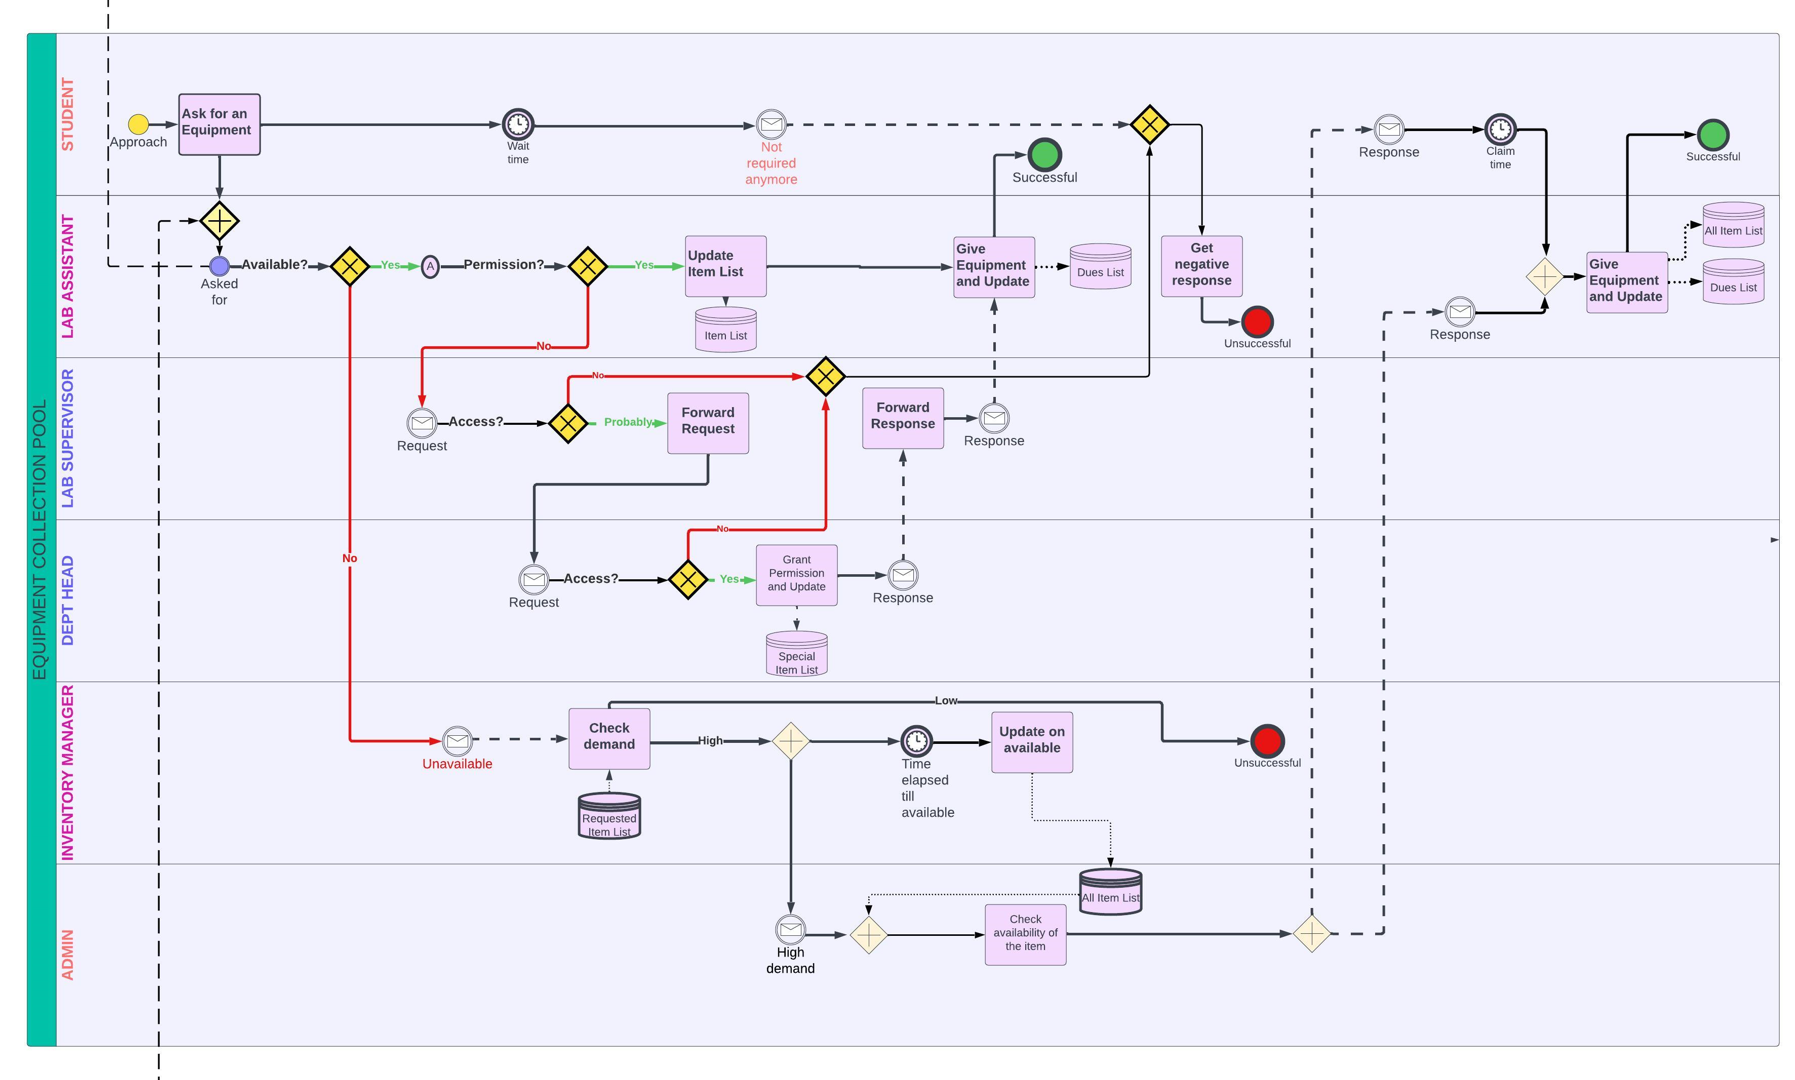
\includegraphics[width= 0.9\textwidth , height= 0.4\paperheight]{Pool1.png}
        \caption{{The Equipment Collection Pool}}
        \label{fig:1}
    \end{figure}

\end{frame}

\begin{frame}{Inventory and Stock Maintenance Pool}

    \begin{alertblock}{Properties and Connectivities}

    \vspace{10}

    \justifying{The Inventory and Stock Maintenance pool responds to the pool of Equipment Collection. This pool is supposed to represent a frequently running process, as maintenance is spontaneous .}

    \vspace{10}

    \end{alertblock}

    \begin{figure}
        \centering
        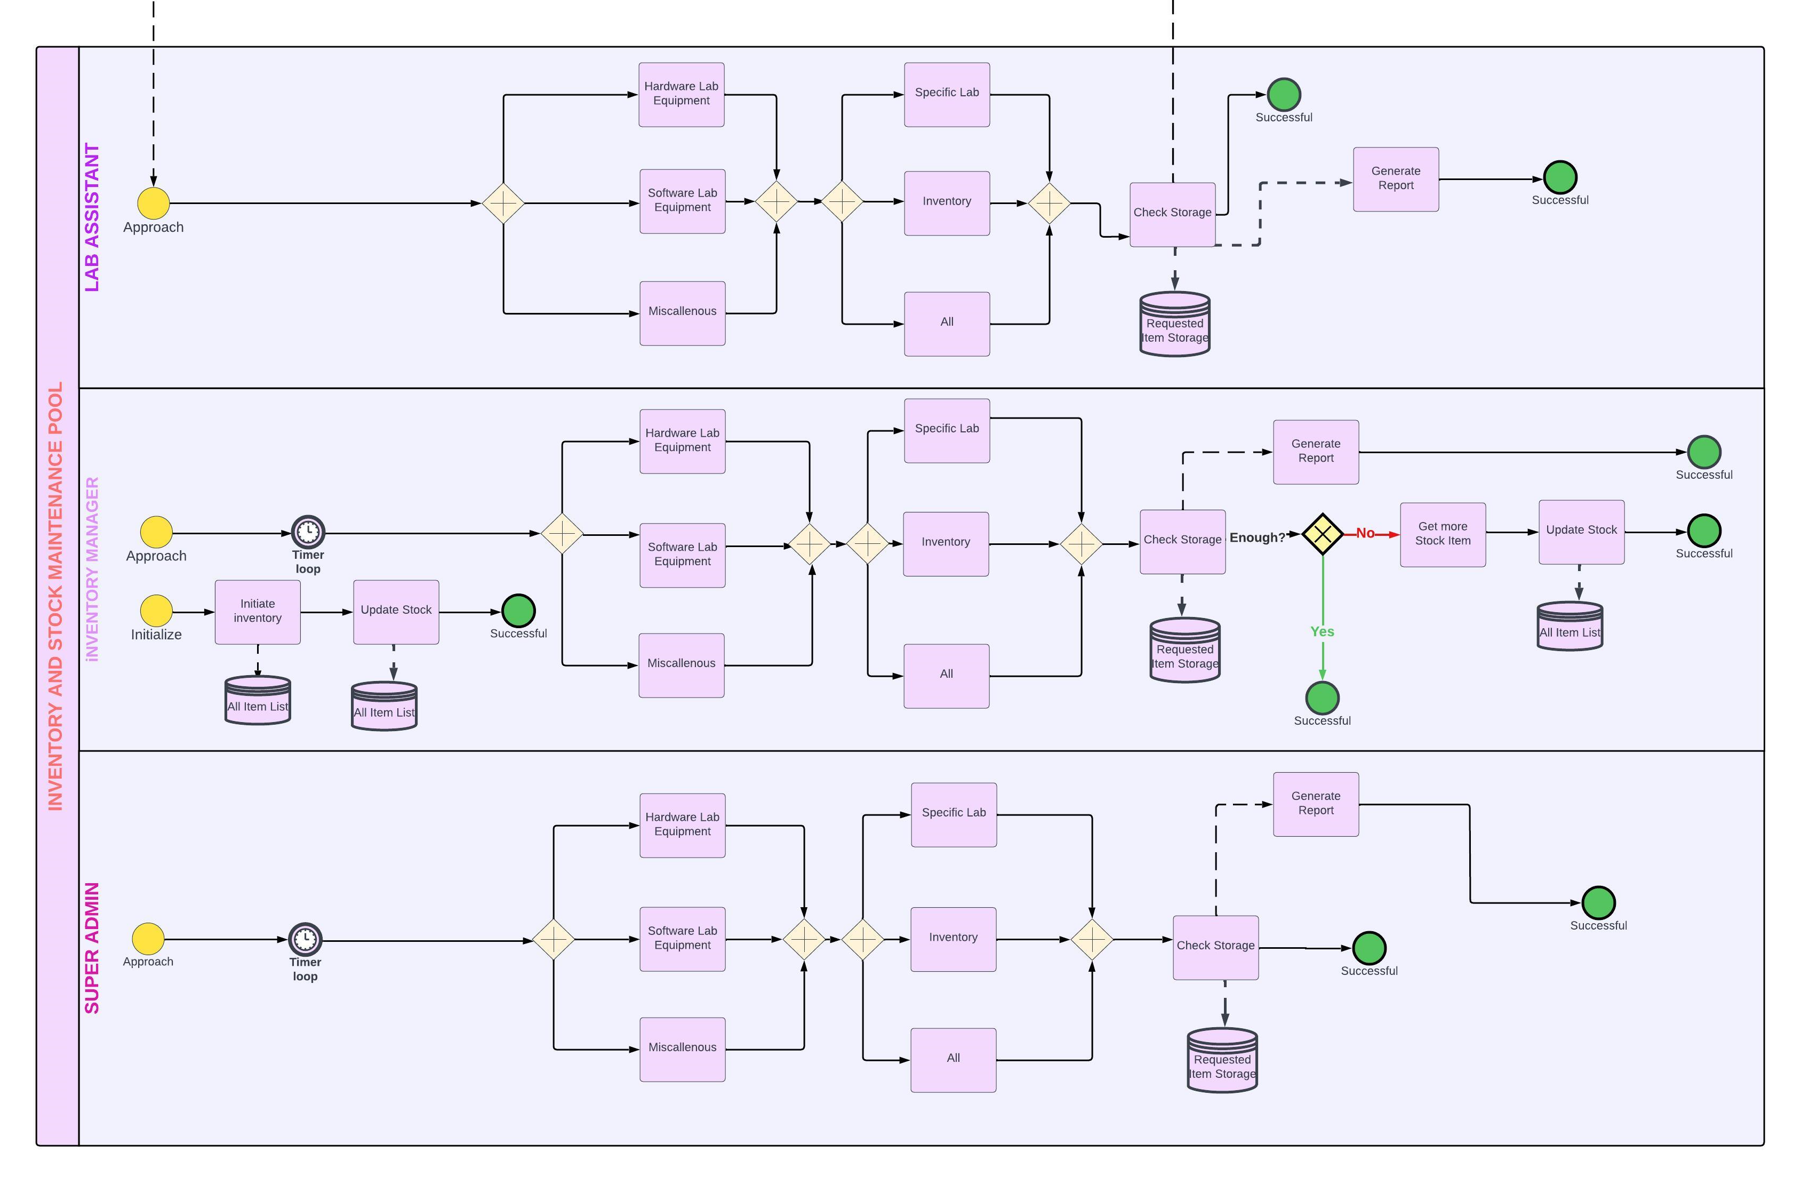
\includegraphics[width= 0.9\textwidth , height= 0.4\paperheight]{Pool2.png}
        \caption{{The Inventory and Stock Maintenance Pool}}
        \label{fig:2}
    \end{figure}

\end{frame}

\begin{frame}{Dues Status Pool and Clearance Pool}

    \begin{alertblock}{Properties and Connectivities}

    \vspace{10}

     \justifying{This pool maintains a relation among student, lab assistant and the superadmin , where the student can check dues and communicate with lab assistant for clearing dues, or lost and damaged stuff. And the lab assistant communicates with superadmin for the clearance of any student. Moreover, the lab assistant, at a regular interval of 14 days, can notify students of their pending equipments to return.}

     \vspace{10}

    \end{alertblock}

    \begin{figure}
        \centering
        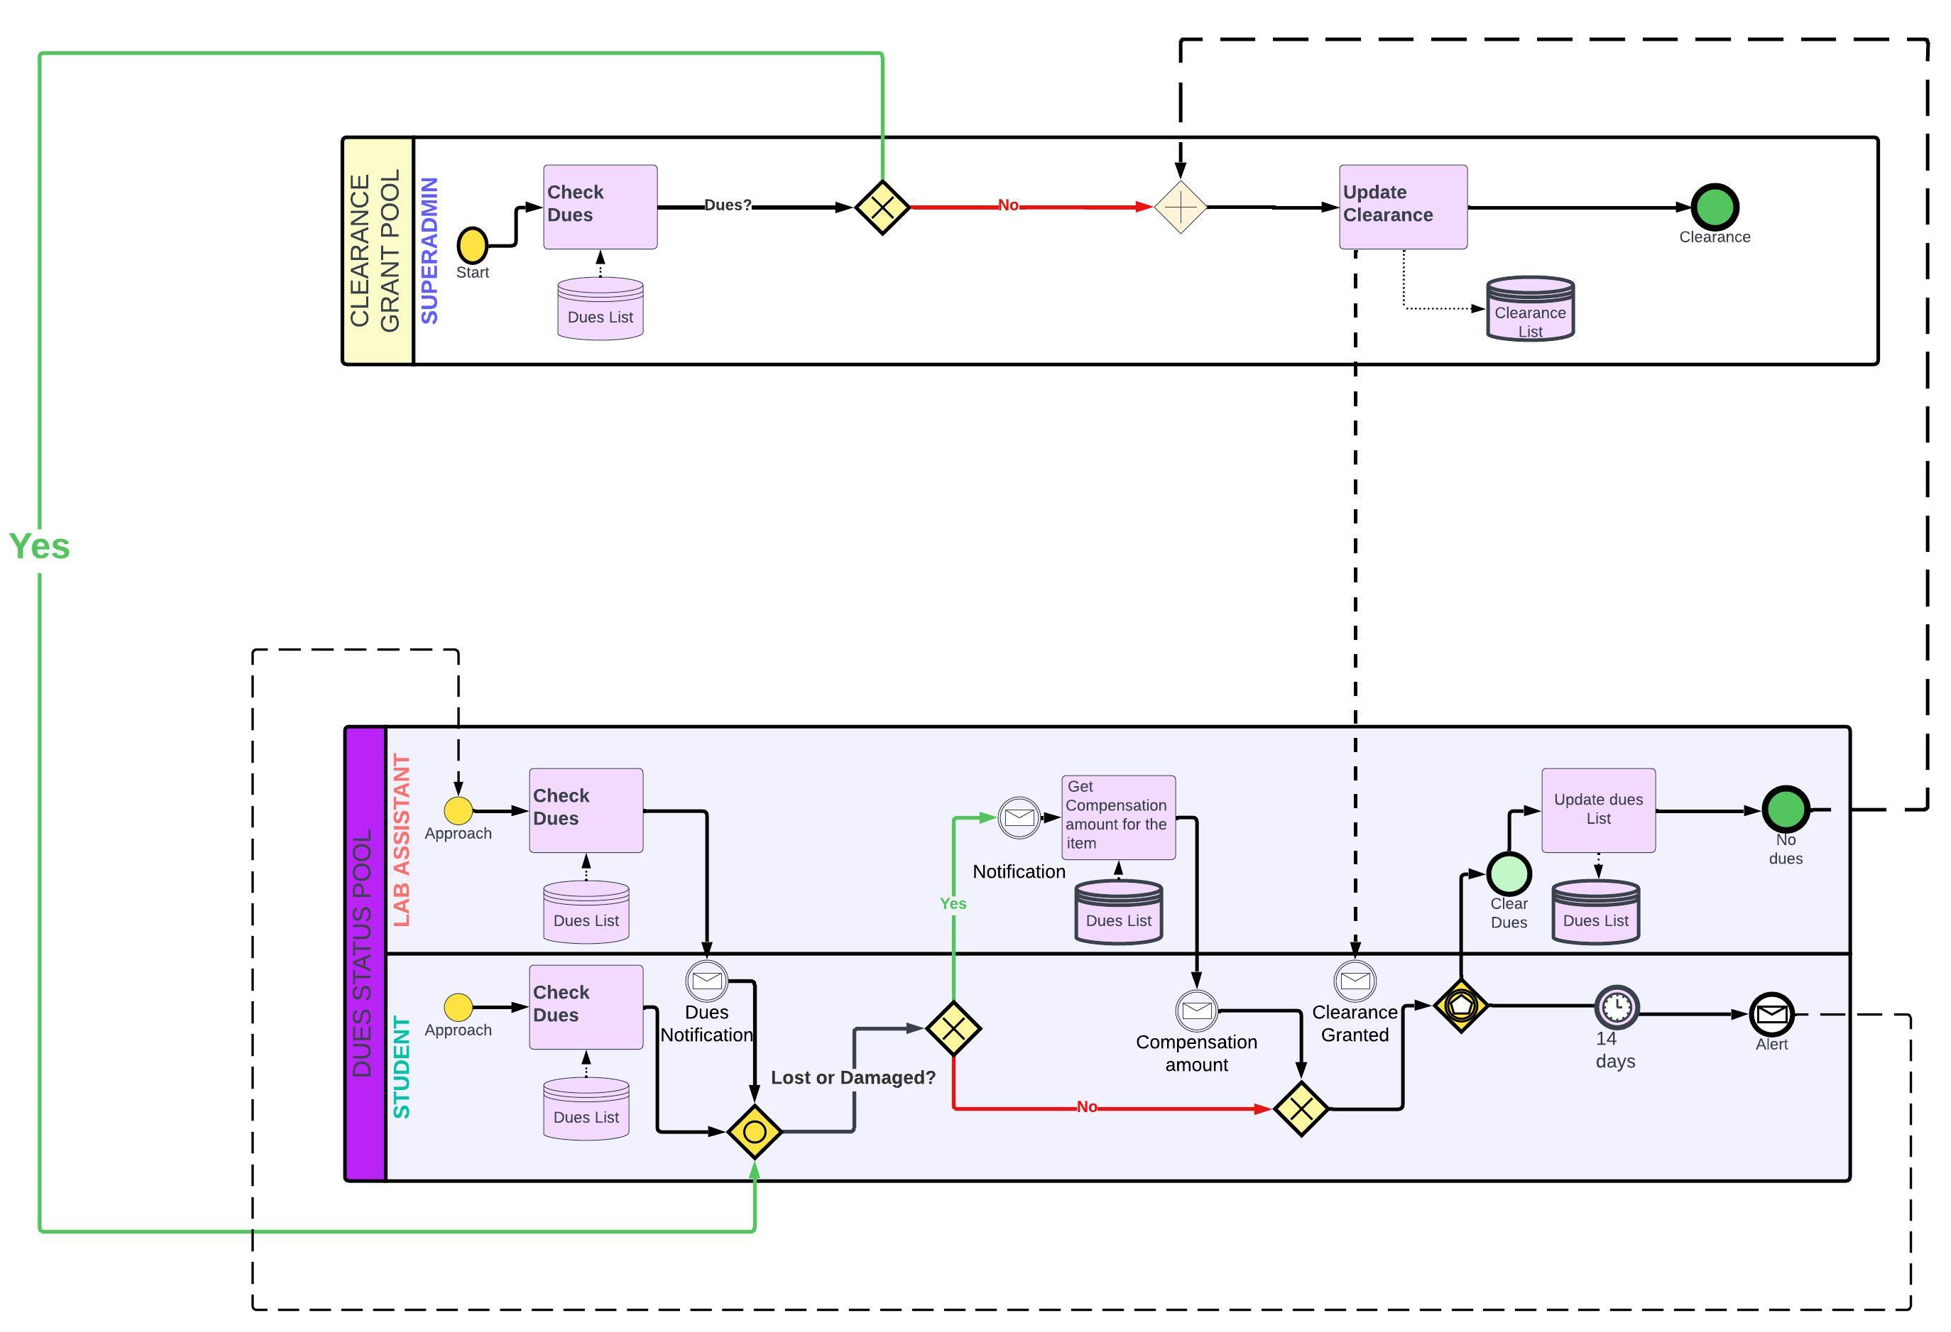
\includegraphics[width= 0.9\textwidth , height= 0.4\paperheight]{Pool3R4.png}
        \caption{{The Dues Status Pool and Clearance Grant Pool}}
        \label{fig:3}
    \end{figure}

\end{frame}

\section{Mock User Interface}

\begin{frame}{The Register Page}

     \begin{figure}
        \centering
        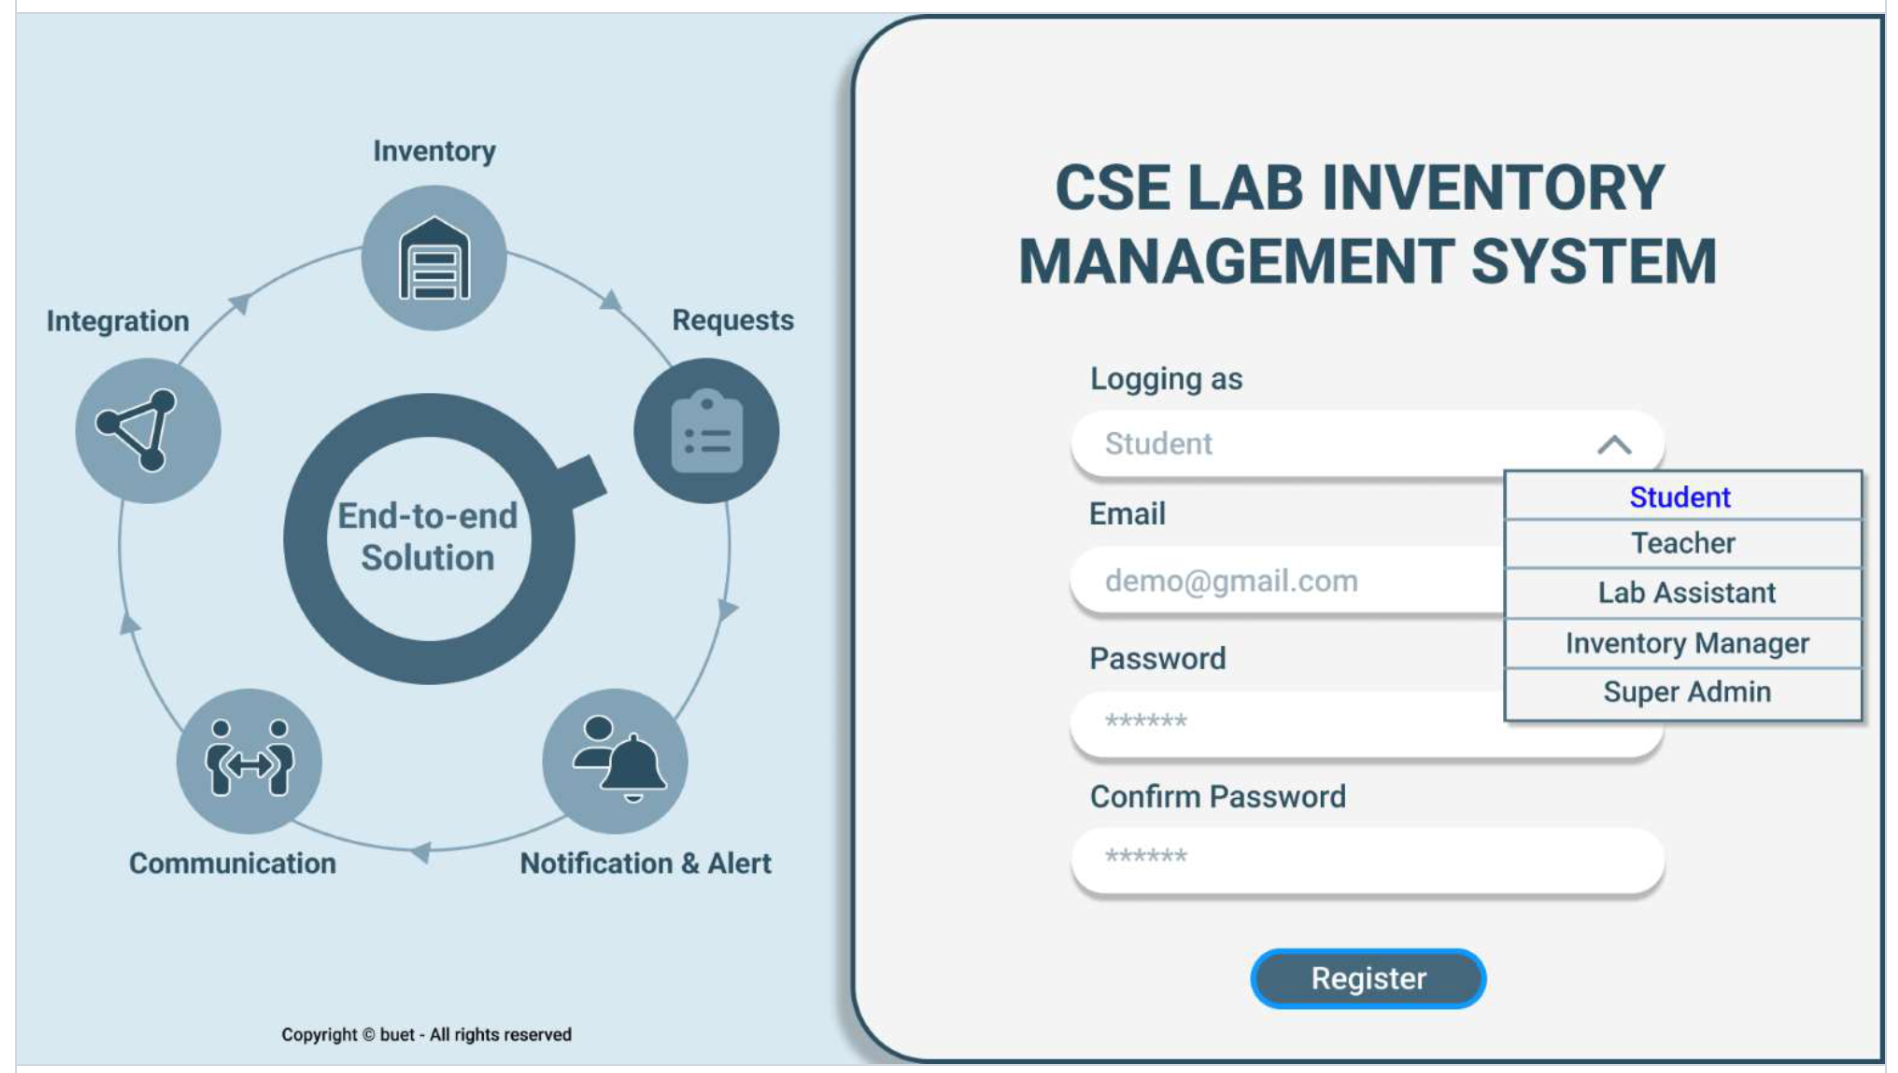
\includegraphics[width= 0.9\textwidth , height= 0.5\paperheight]{RegisterUI.png}
        \caption{Registration Page}
        \label{fig:50}
    \end{figure}

\end{frame}

\begin{frame}{The Login Page}

     \begin{figure}
        \centering
        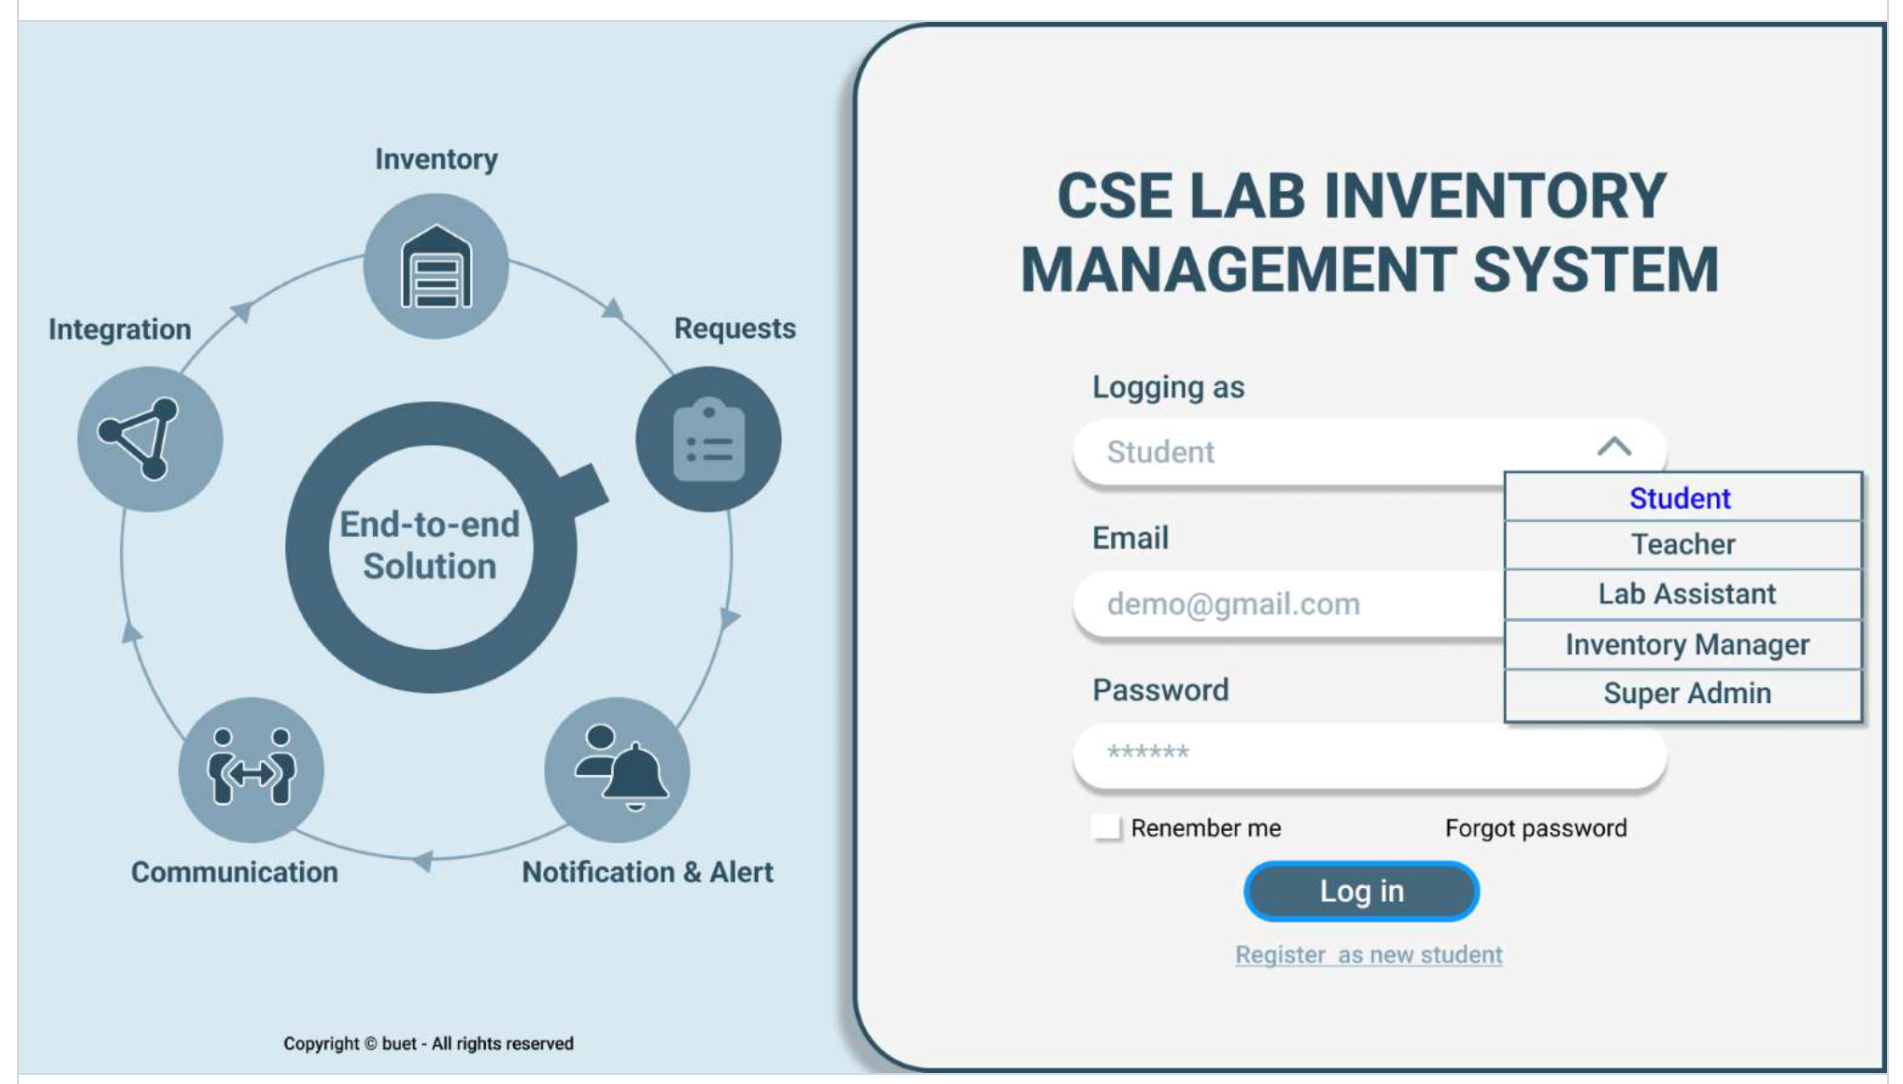
\includegraphics[width= 0.9\textwidth , height= 0.5\paperheight]{LoginUI.png}
        \caption{Login Page}
        \label{fig:51}
    \end{figure}

\end{frame}

\subsection{Students' End}

\begin{frame}{The Student Home Page}

     \begin{figure}
        \centering
        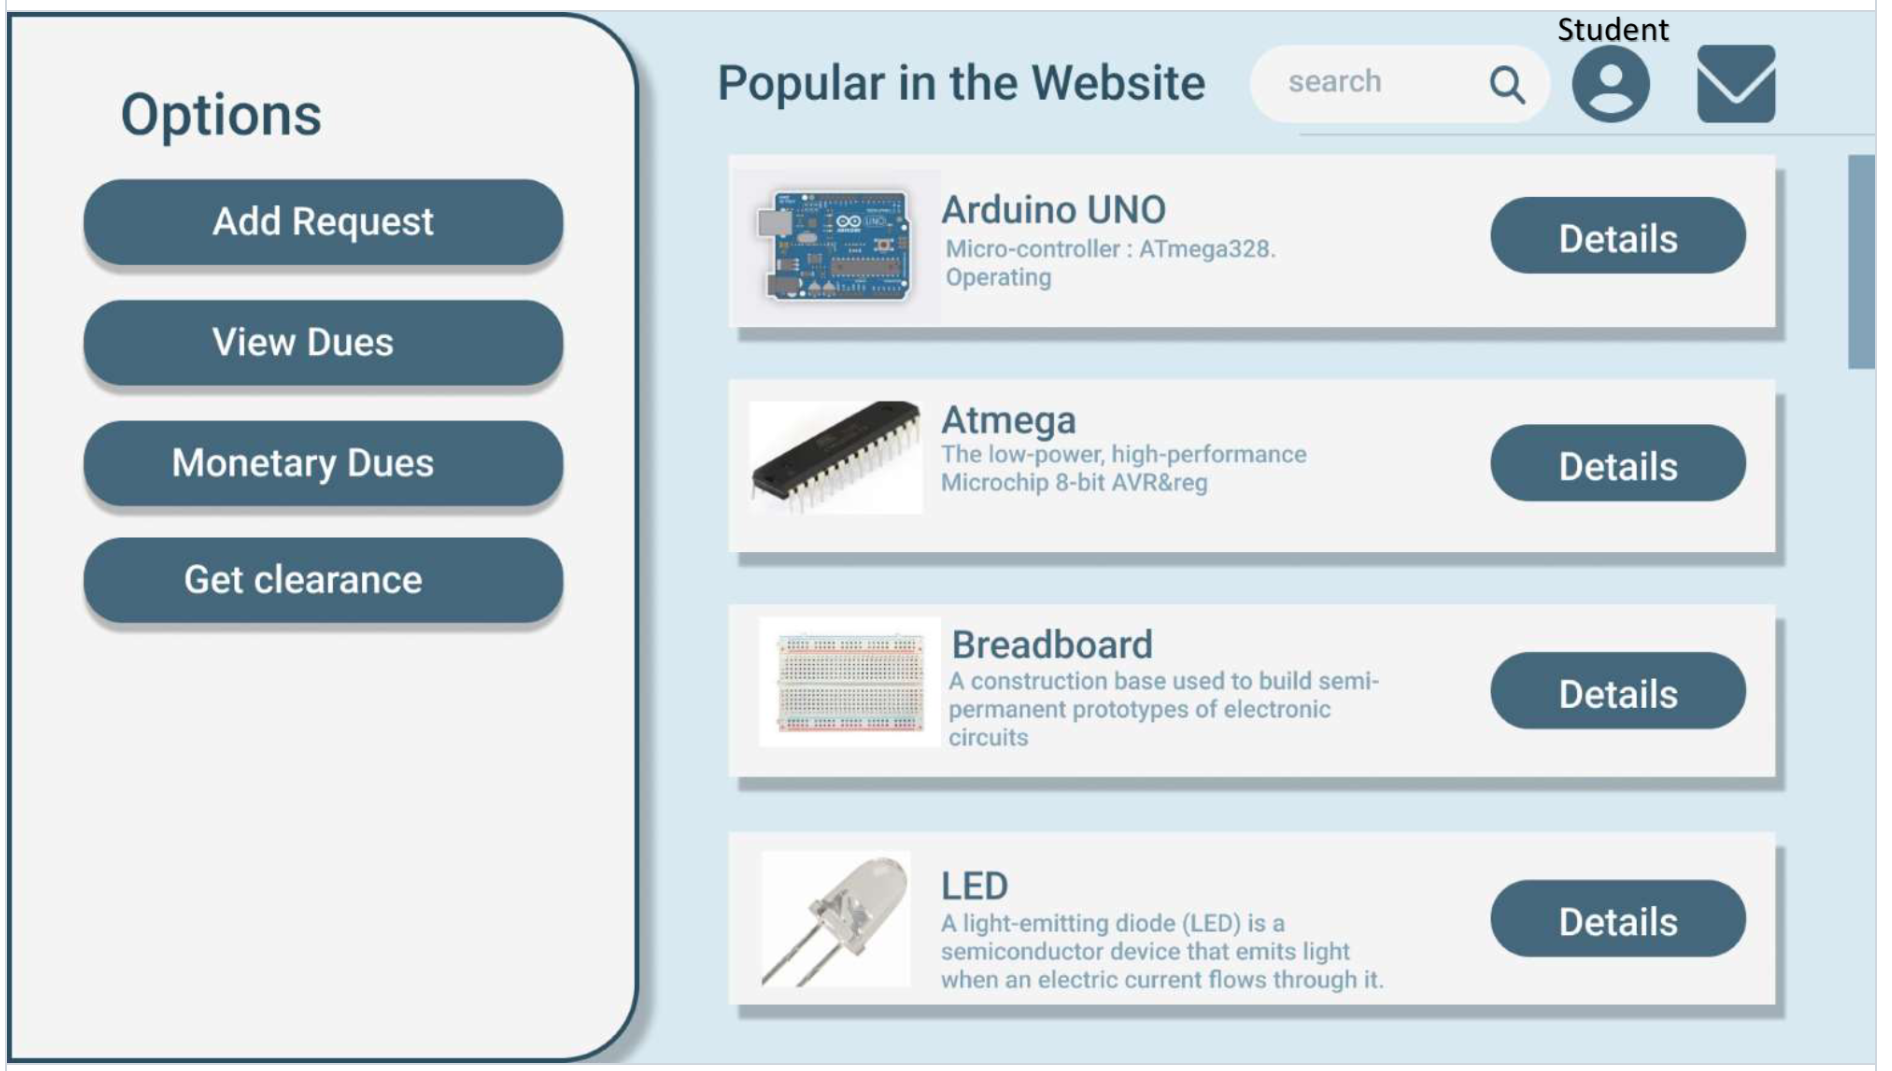
\includegraphics[width= 0.9\textwidth , height= 0.5\paperheight]{StudentHomeUI.png}
        \caption{Home Page from students' end}
        \label{fig:52}
    \end{figure}

\end{frame}

\begin{frame}{The Product Page}

     \begin{figure}
        \centering
        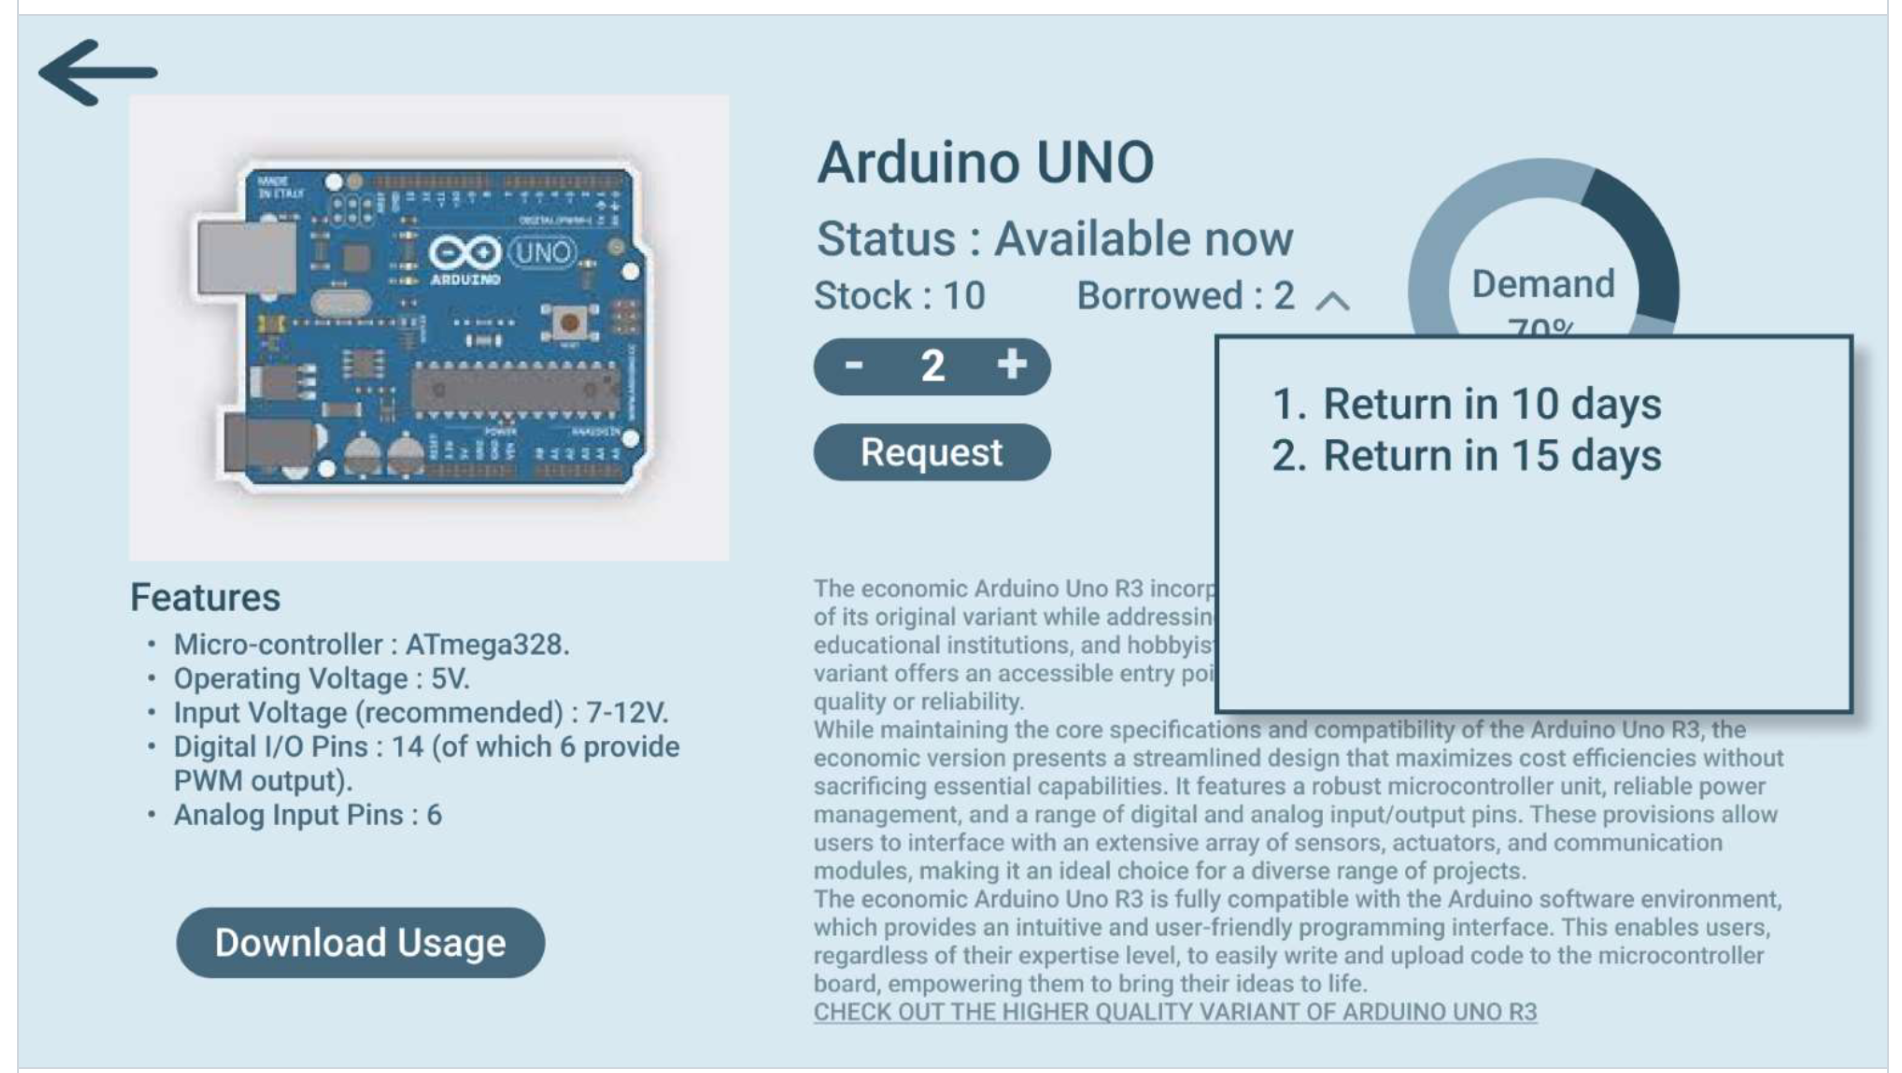
\includegraphics[width= 0.9\textwidth , height= 0.5\paperheight]{ProductUI.png}
        \caption{Product Page}
        \label{fig:53}
    \end{figure}

\end{frame}

\begin{frame}{The Dues Page from Students' end}

    \begin{figure}

        \centering

        \begin{minipage}[b]{0.45\textwidth}
            \centering
            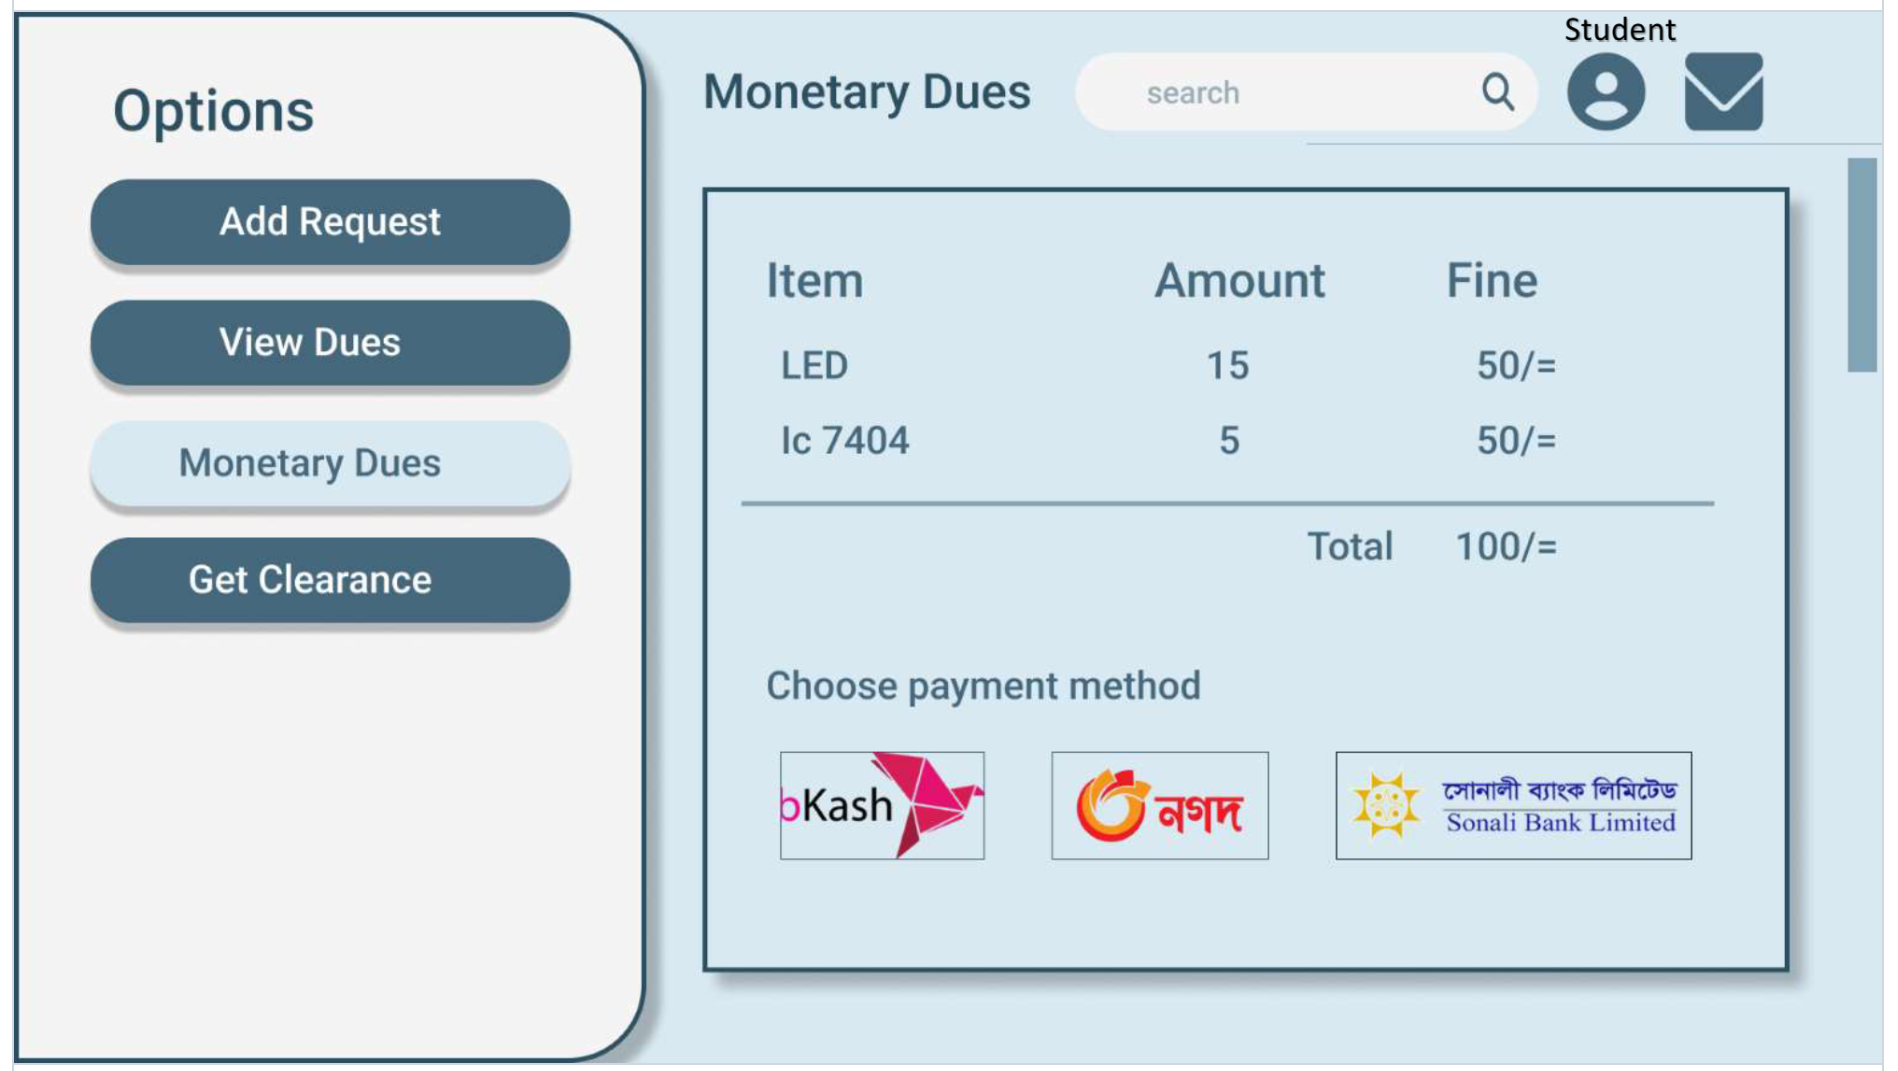
\includegraphics[width= \textwidth , height= 0.2\paperheight]{ViewDuesUI4.png}
            \caption{Monetary Dues}
            \label{fig:54}
        \end{minipage}
        \begin{minipage}[b]{0.45\textwidth}
            \centering
            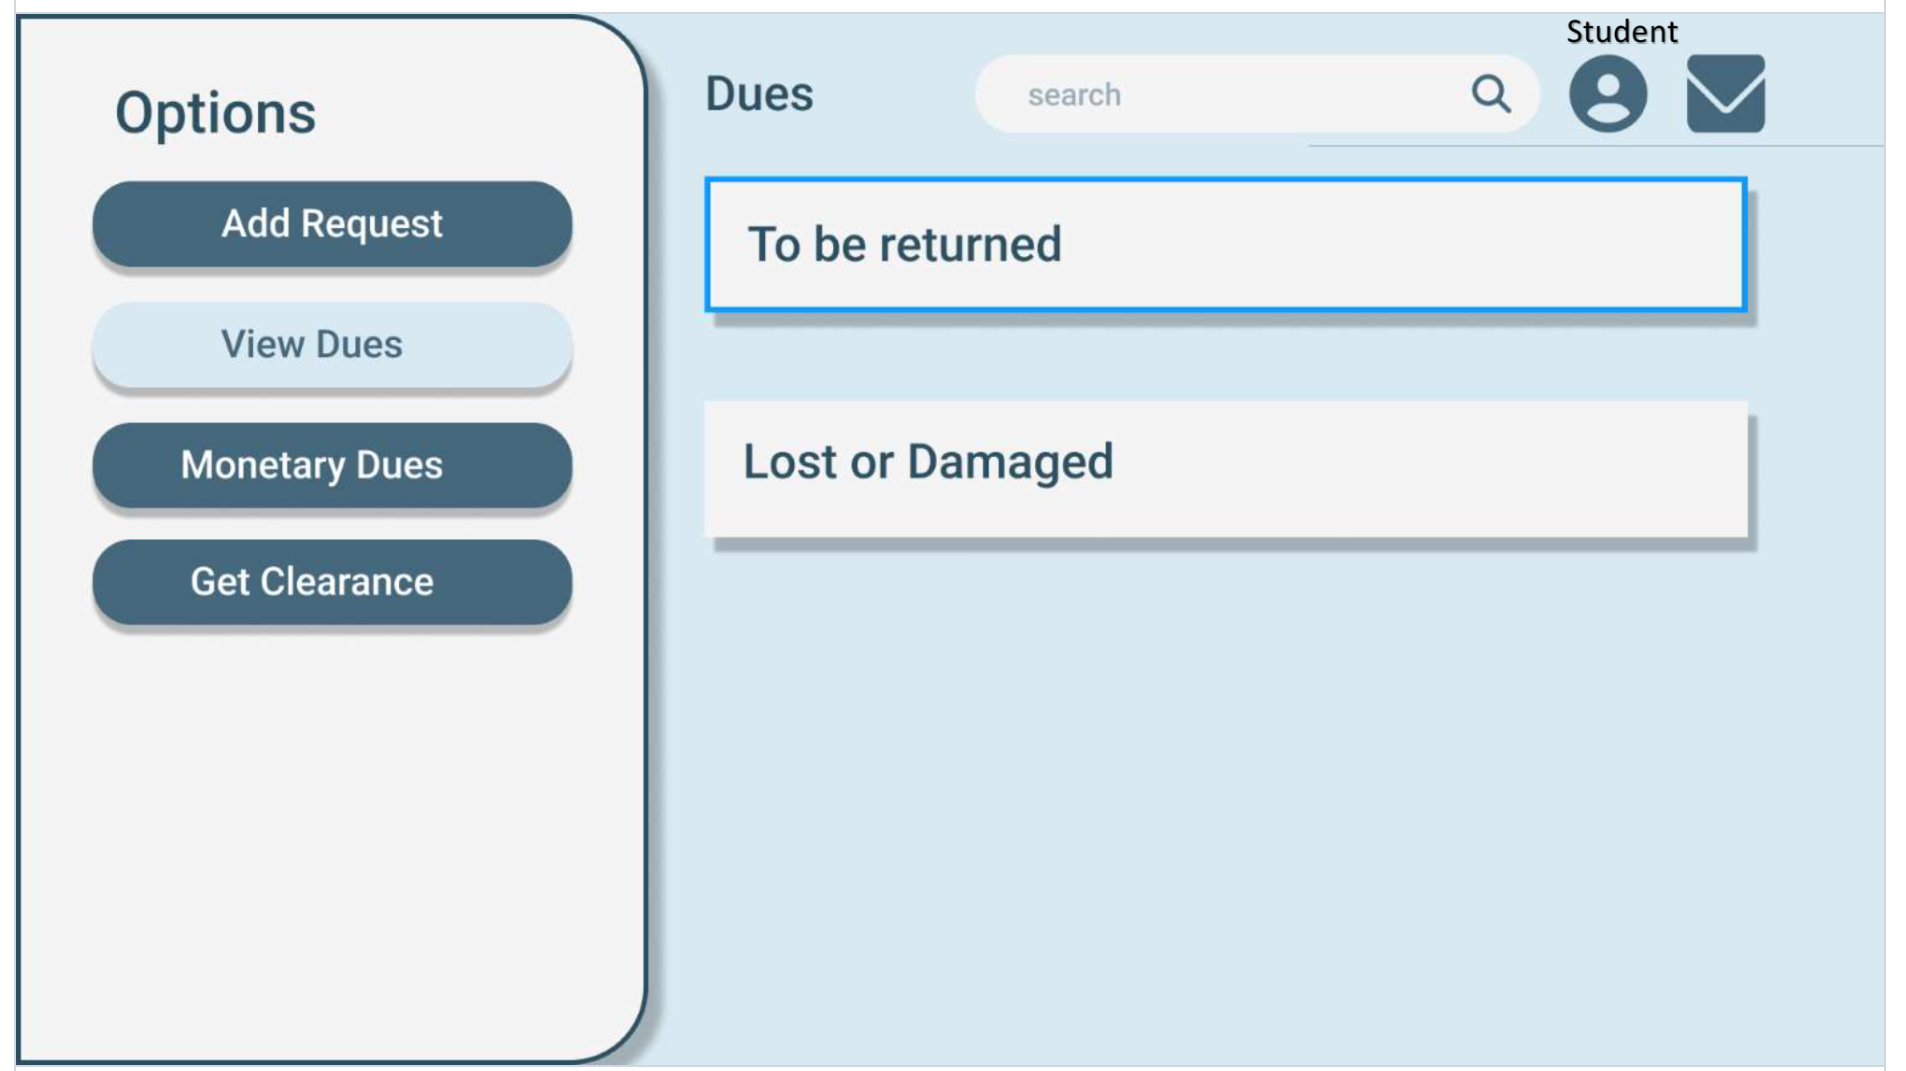
\includegraphics[width= \textwidth , height= 0.2\paperheight]{ViewDuesUI.png}
            \caption{View Dues}
            \label{fig:55}

        \end{minipage}
        
    \end{figure}

    

    \begin{figure}

        \centering

        \begin{minipage}[b]{0.45\textwidth}
            \centering
            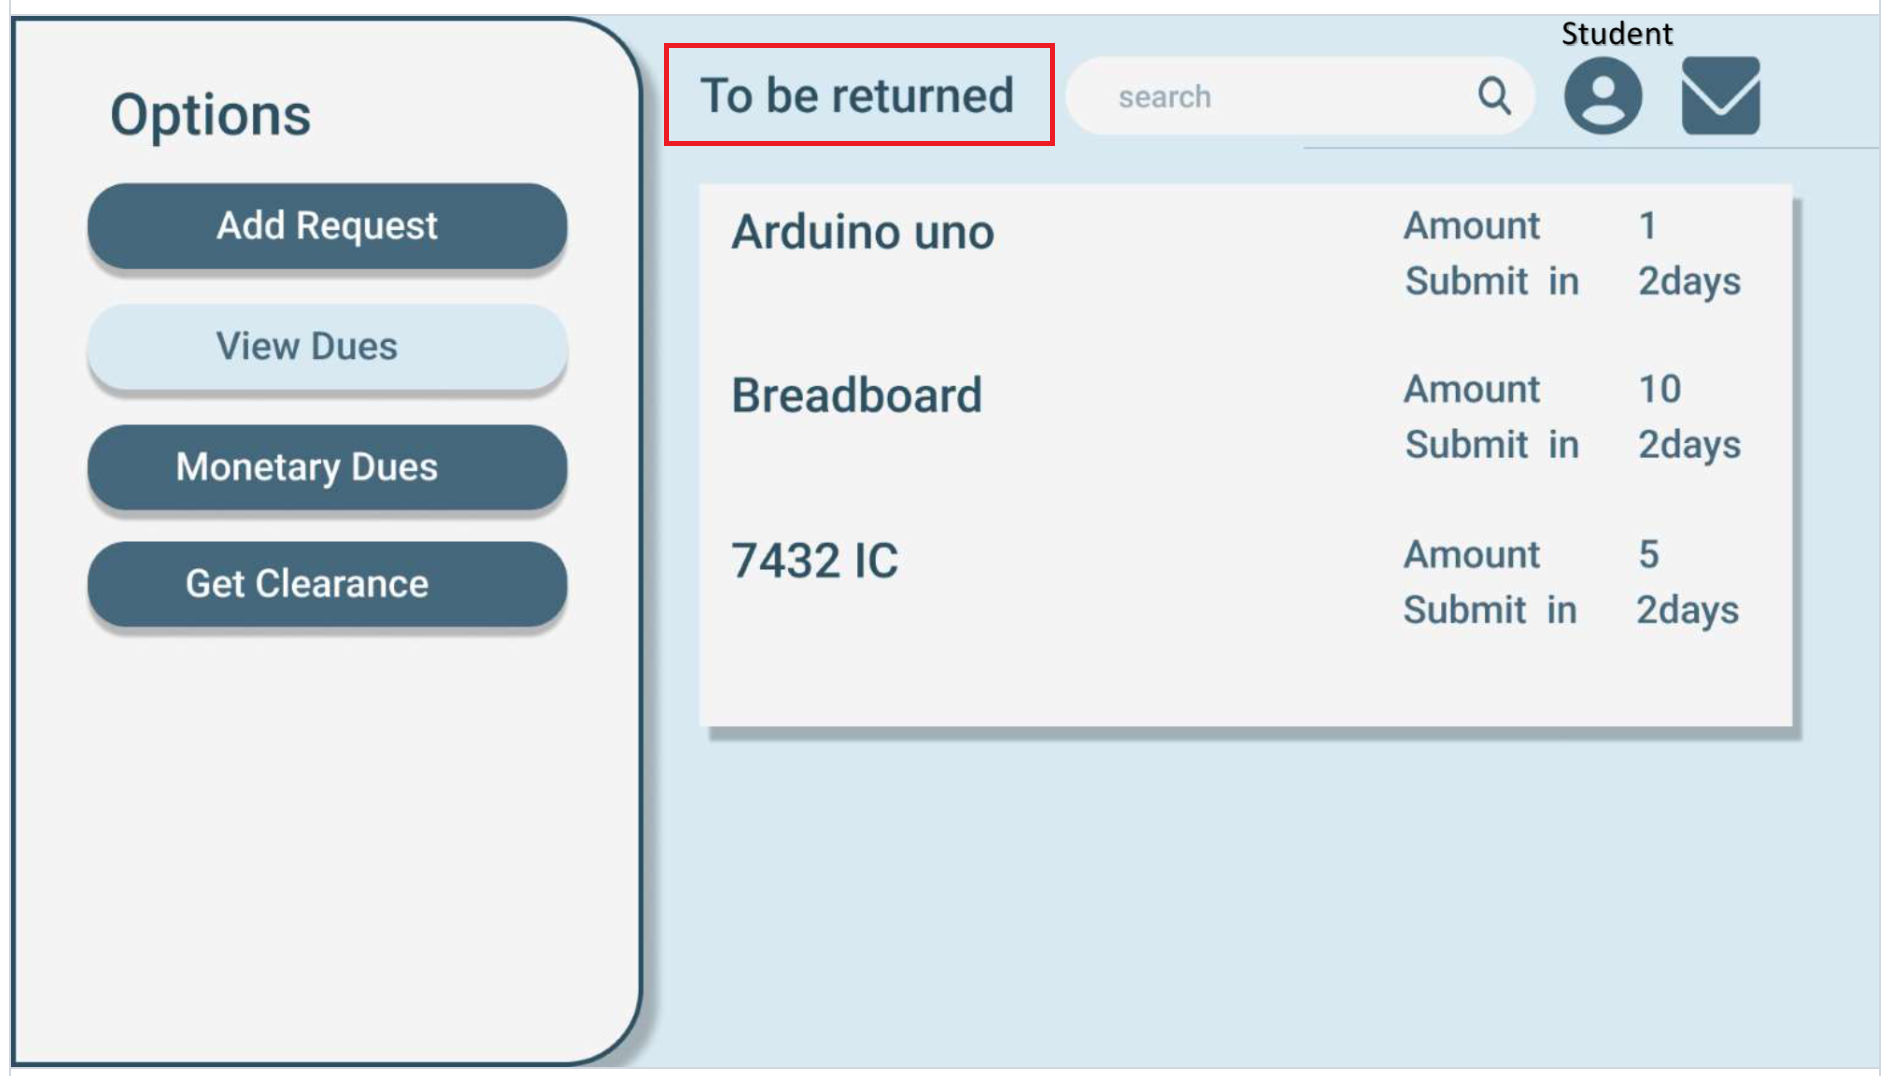
\includegraphics[width= \textwidth , height= 0.2\paperheight]{ViewDuesUI2.png}
            \caption{Goods to be returned}
            \label{fig:56}
        \end{minipage}
        \begin{minipage}[b]{0.45\textwidth}
            \centering
            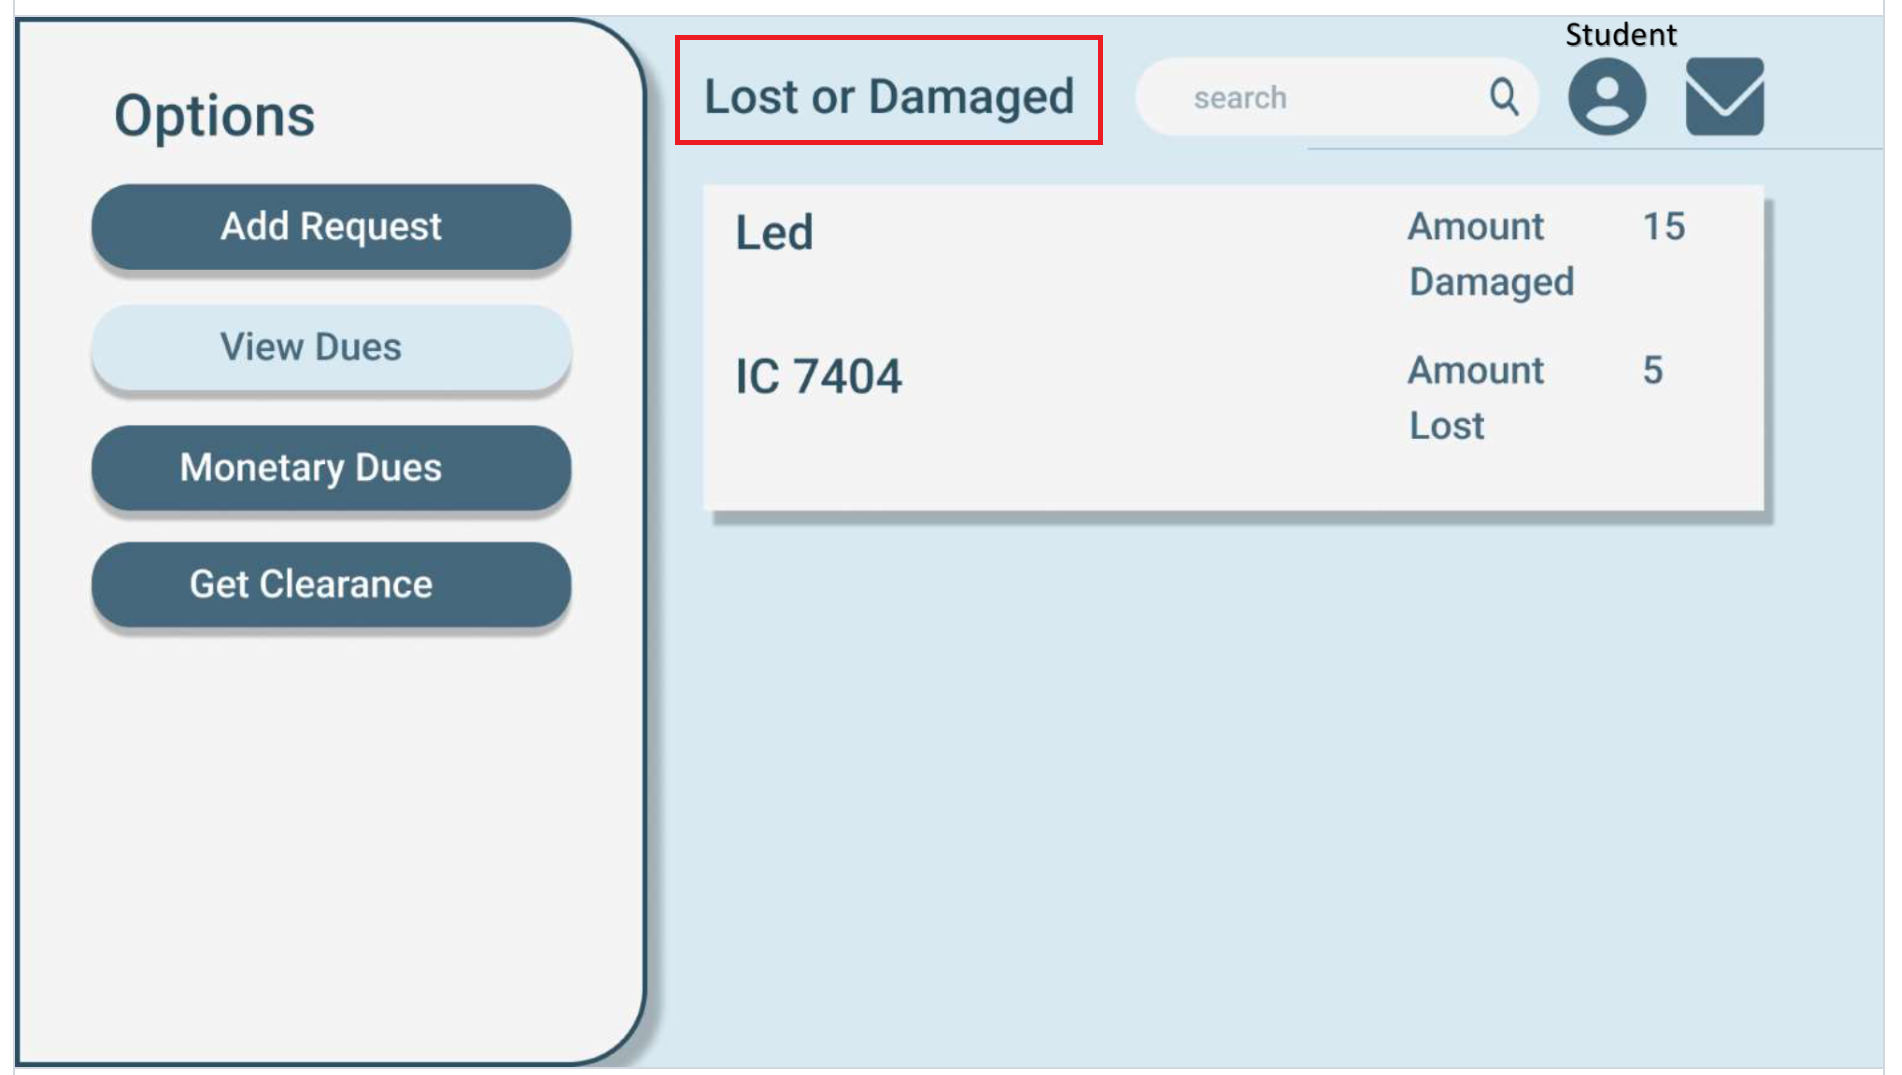
\includegraphics[width= \textwidth , height= 0.2\paperheight]{ViewDuesUI3.png}
            \caption{Goods lost or damaged}
            \label{fig:57}

        \end{minipage}
        
    \end{figure}

\end{frame}

\begin{frame}{The Students' Clearance Page}

     \begin{figure}
        \centering
        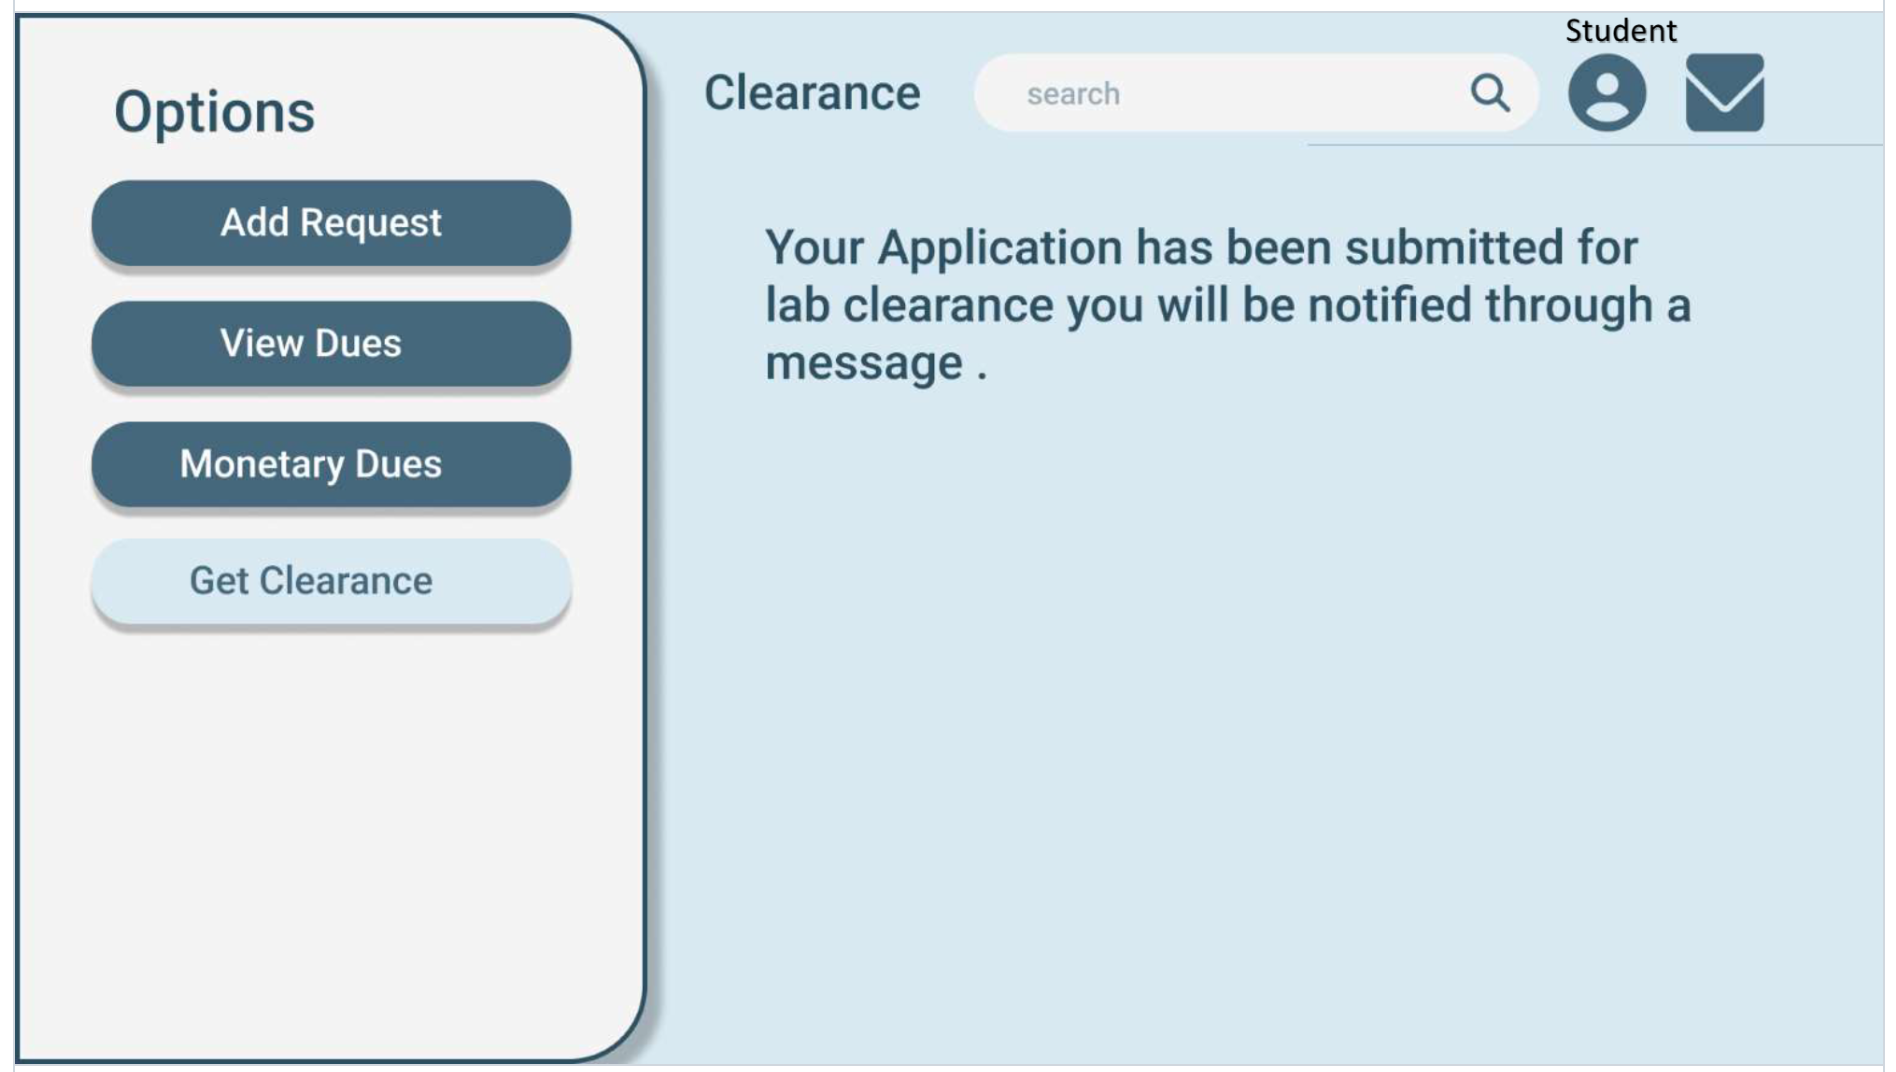
\includegraphics[width= 0.9\textwidth , height= 0.5\paperheight]{SudentClearanceUI.png}
        \caption{Page for getting clearance}
        \label{fig:58}
    \end{figure}

\end{frame}

\subsection{Response End}

\begin{frame}{The View Request Page}

    \begin{block}{About this page}

    \vspace{10}

    \justifying{The page for viewing requests of any student is only for lab assistant, inventory manager and the authorized faculty. Those who have direct access to inventory stuff can handle requests only.}

    \vspace{10}

    \end{block}

     \begin{figure}
        \centering
        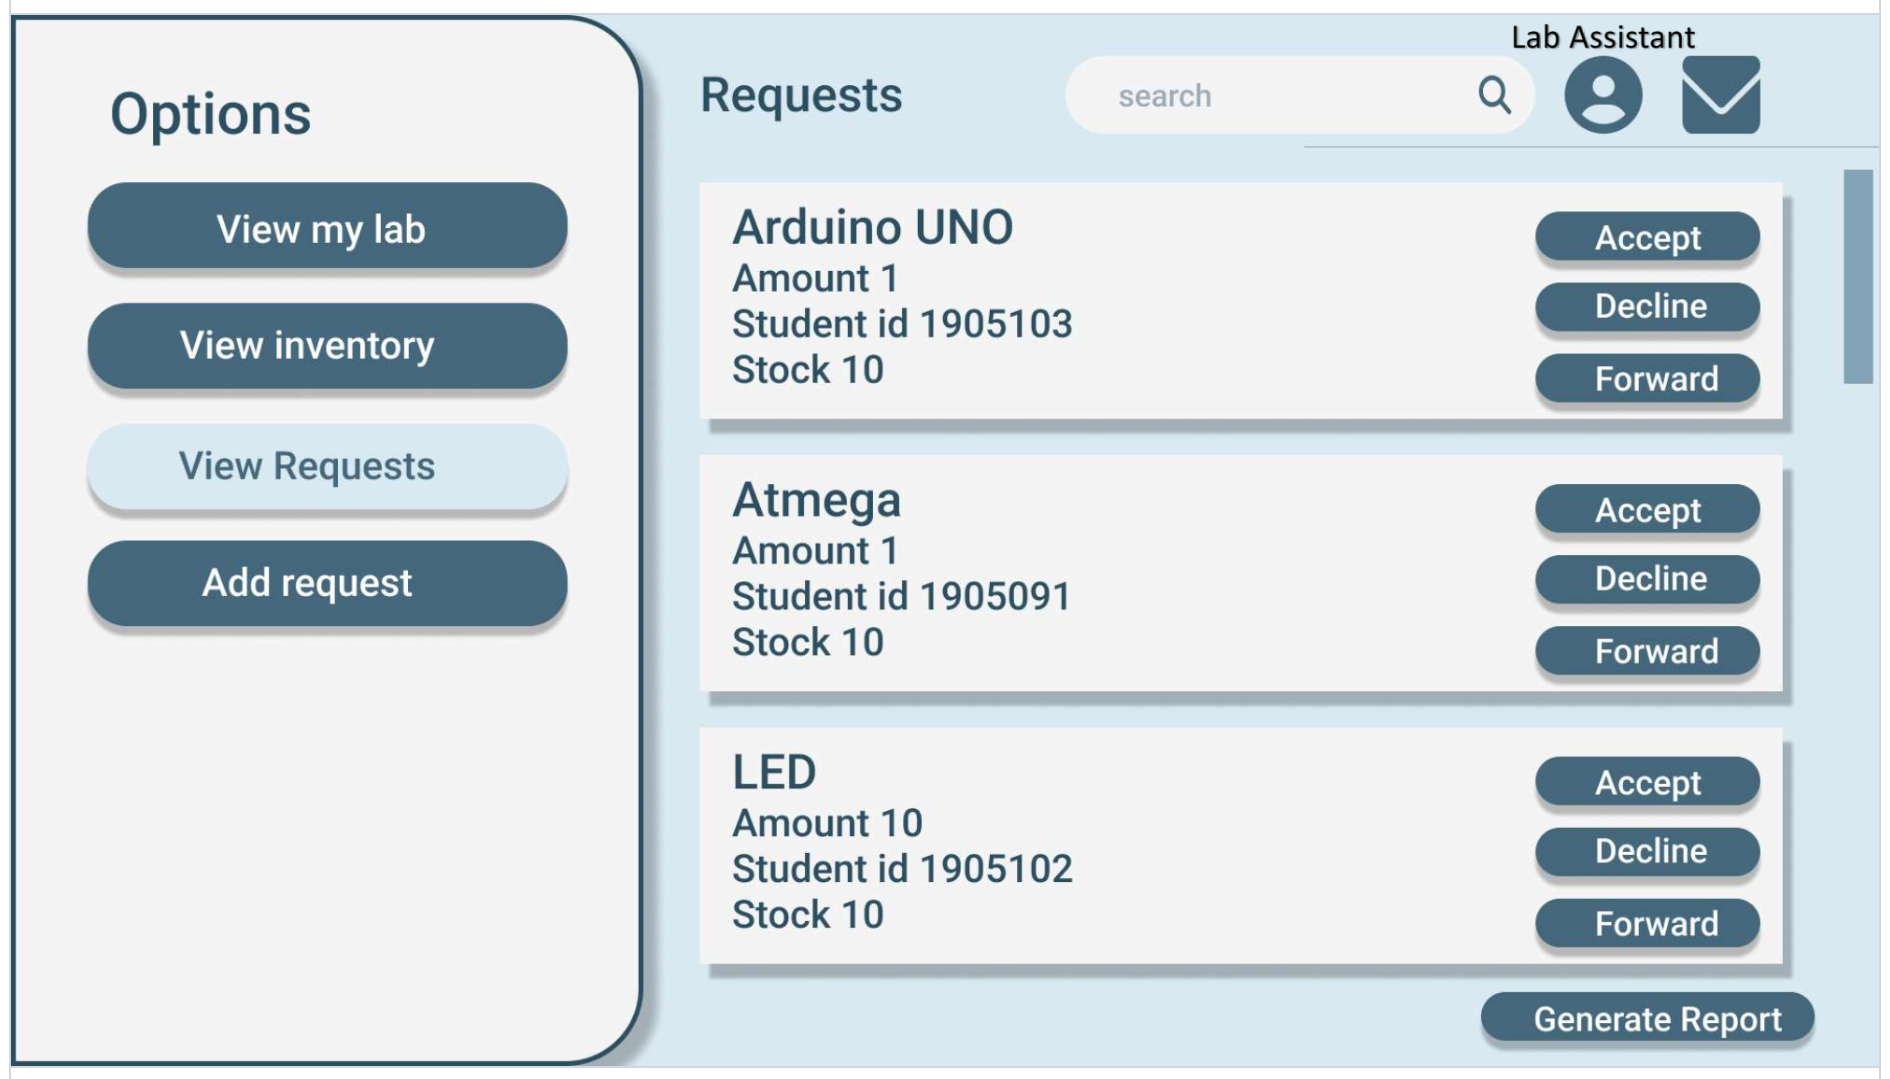
\includegraphics[width= 0.9\textwidth , height= 0.5\paperheight]{ViewRequestUI.png}
        \caption{Request Viewing Page}
        \label{fig:59}
    \end{figure}

\end{frame}

\subsection{Lab Assistant End}

\begin{frame}{The Lab Request Page for the end of Lab Assistant}

     \begin{figure}
        \centering
        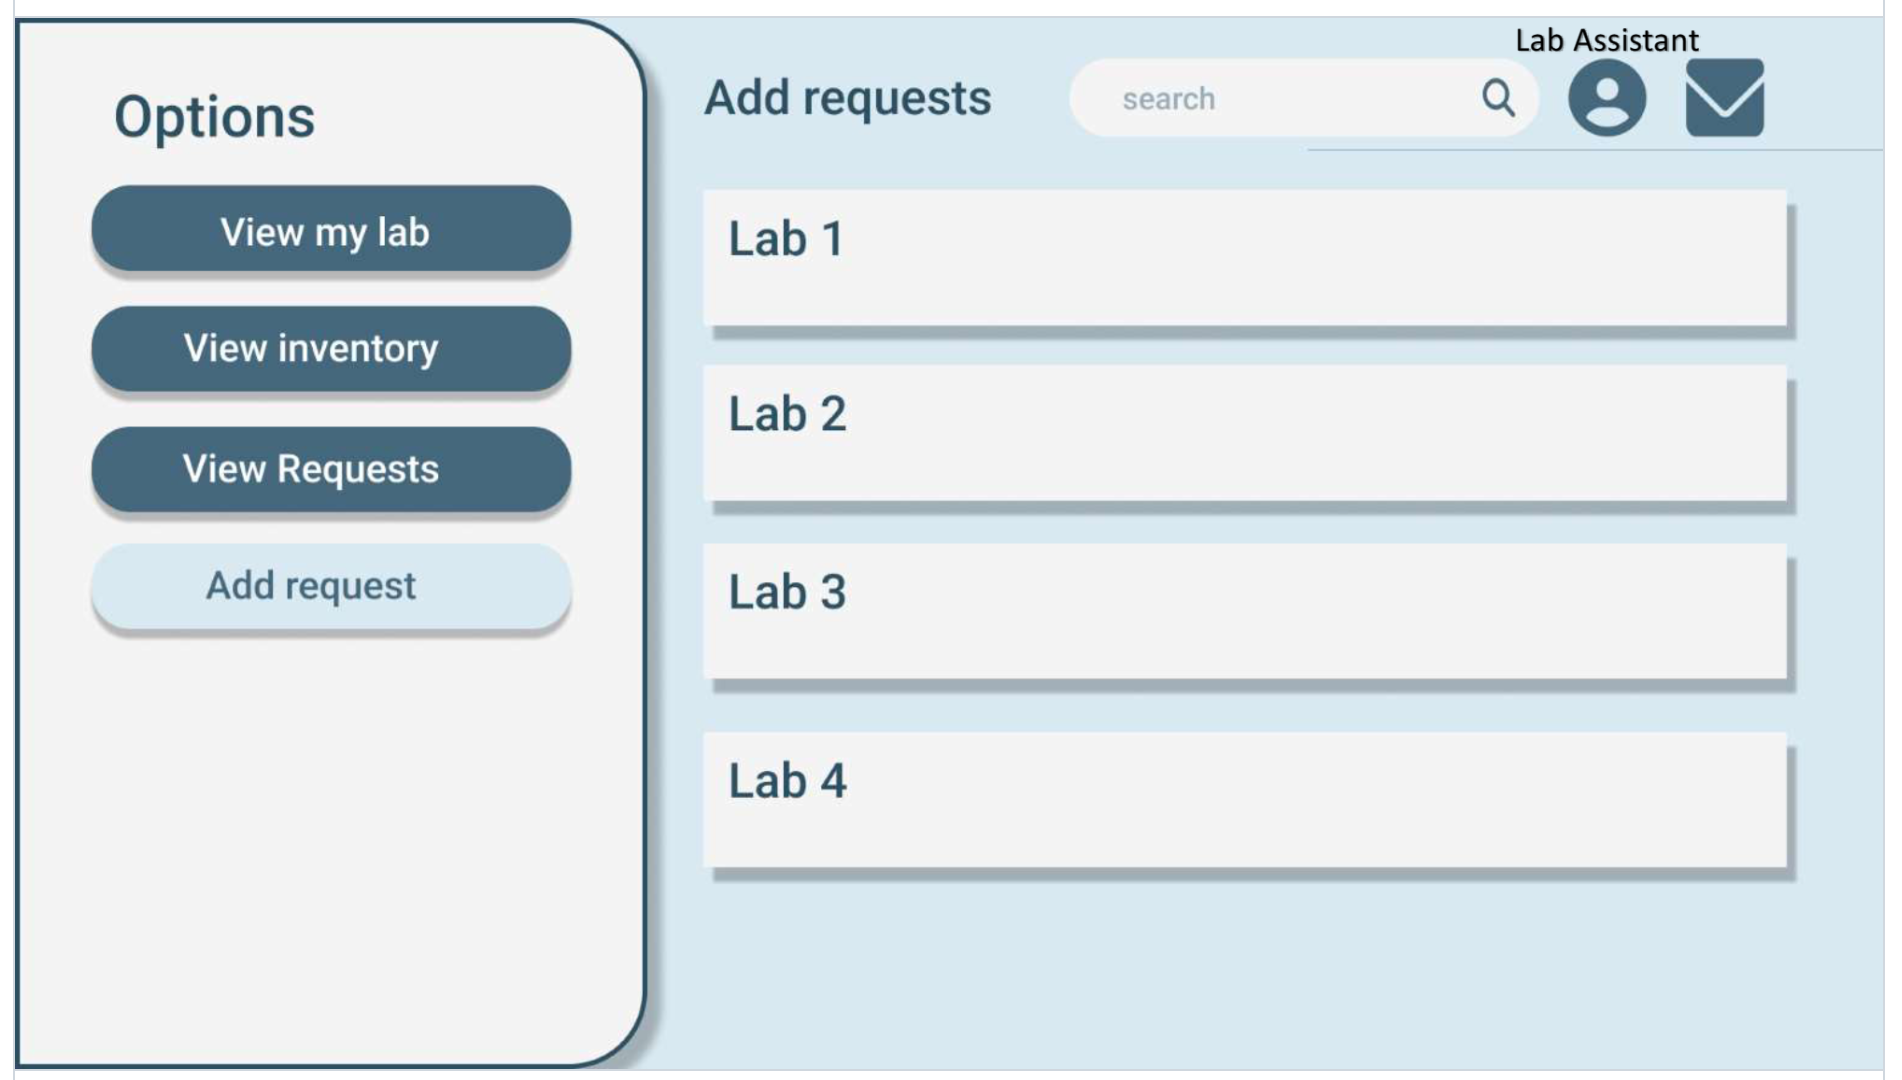
\includegraphics[width= 0.9\textwidth , height= 0.5\paperheight]{LabAssistantAddRequestUI.png}
        \caption{Request Page from the end of Lab Assistant}
        \label{fig:60}
    \end{figure}

\end{frame}

\subsection{Inventory Manager End}

\begin{frame}{The Item Adding Page }

    \begin{block}{About this page}

    \vspace{10}

    \justifying{The page for adding an item is accessible to the Inventory Manager. The inventory manager has a frequent access to checking and updating stock.}

    \vspace{10}

    \end{block}

    \begin{figure}
        \centering
        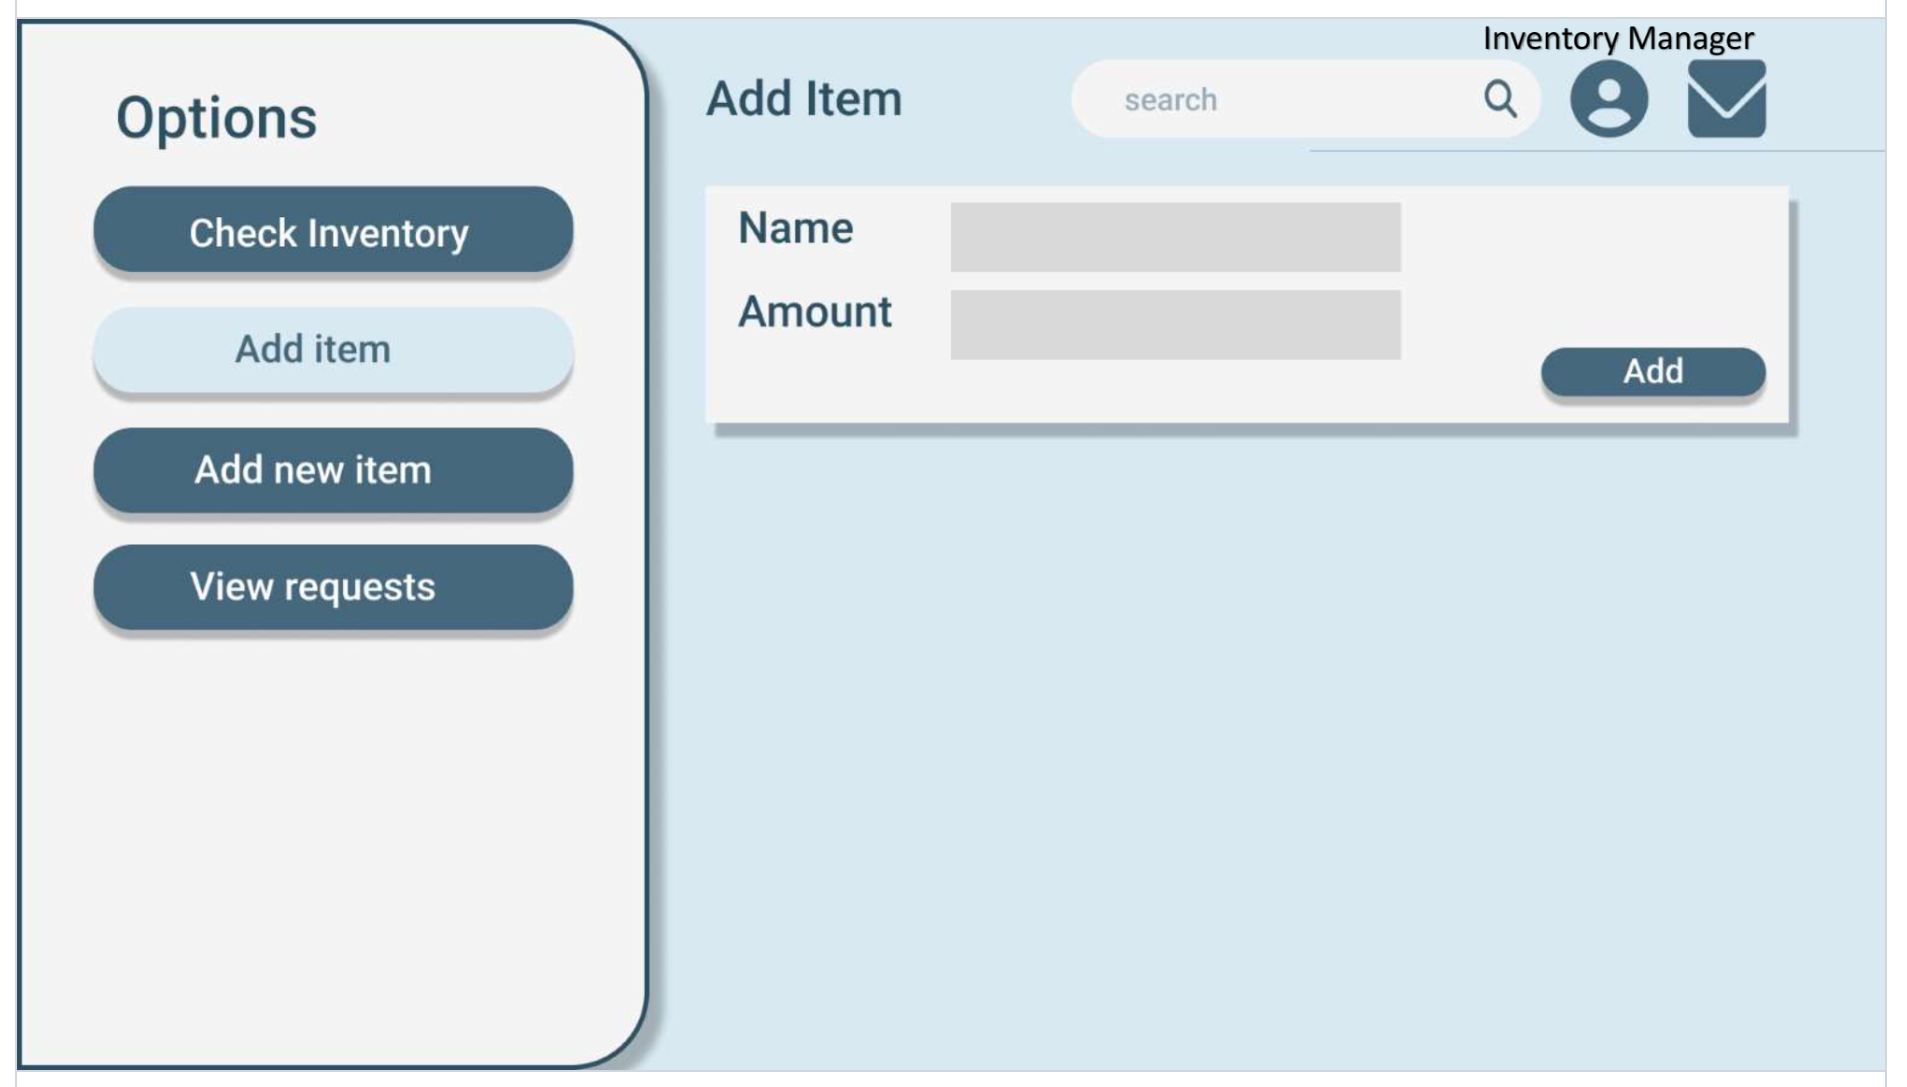
\includegraphics[width= 0.9\textwidth , height= 0.5\paperheight]{InventoryManagerAddItemUI.png}
        \caption{Item Adding Page}
        \label{fig:61}
    \end{figure}

\end{frame}



\begin{frame}{The New Item Adding Page }

    \begin{block}{About this page}

    \vspace{10}

    \justifying{The page for adding a new item is also accessible to the Inventory Manager. This page helps inventory manager to bring new stock. In fact, this page is necessary while initiating the inventory.}

    \vspace{10}

    \end{block}

    \begin{figure}
        \centering
        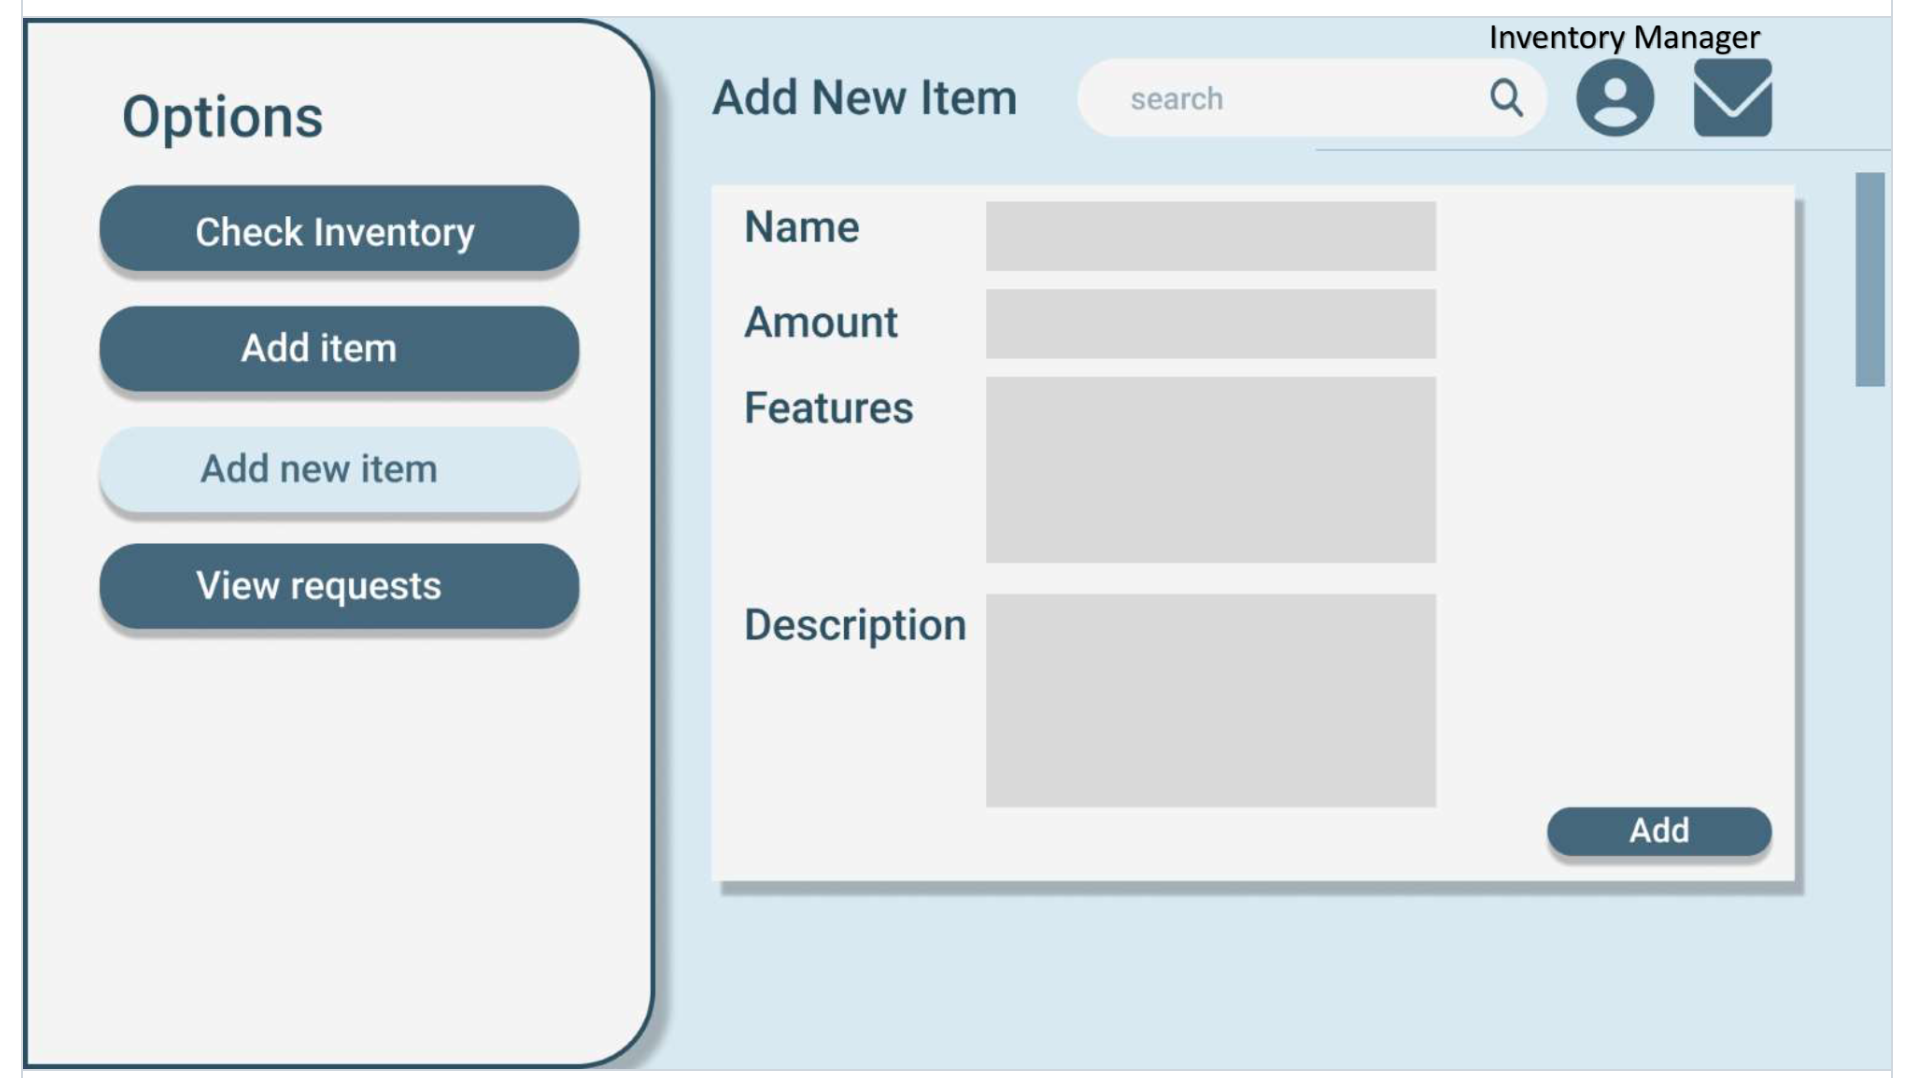
\includegraphics[width= 0.9\textwidth , height= 0.5\paperheight]{InventoryManagerAddNewItemUI.png}
        \caption{Item Adding Page}
        \label{fig:62}
    \end{figure}

\end{frame}

\subsection{SuperAdmin End}

\begin{frame}{The Inventory Checking Page from the end of SuperAdmin}

    \begin{figure}

        \centering
        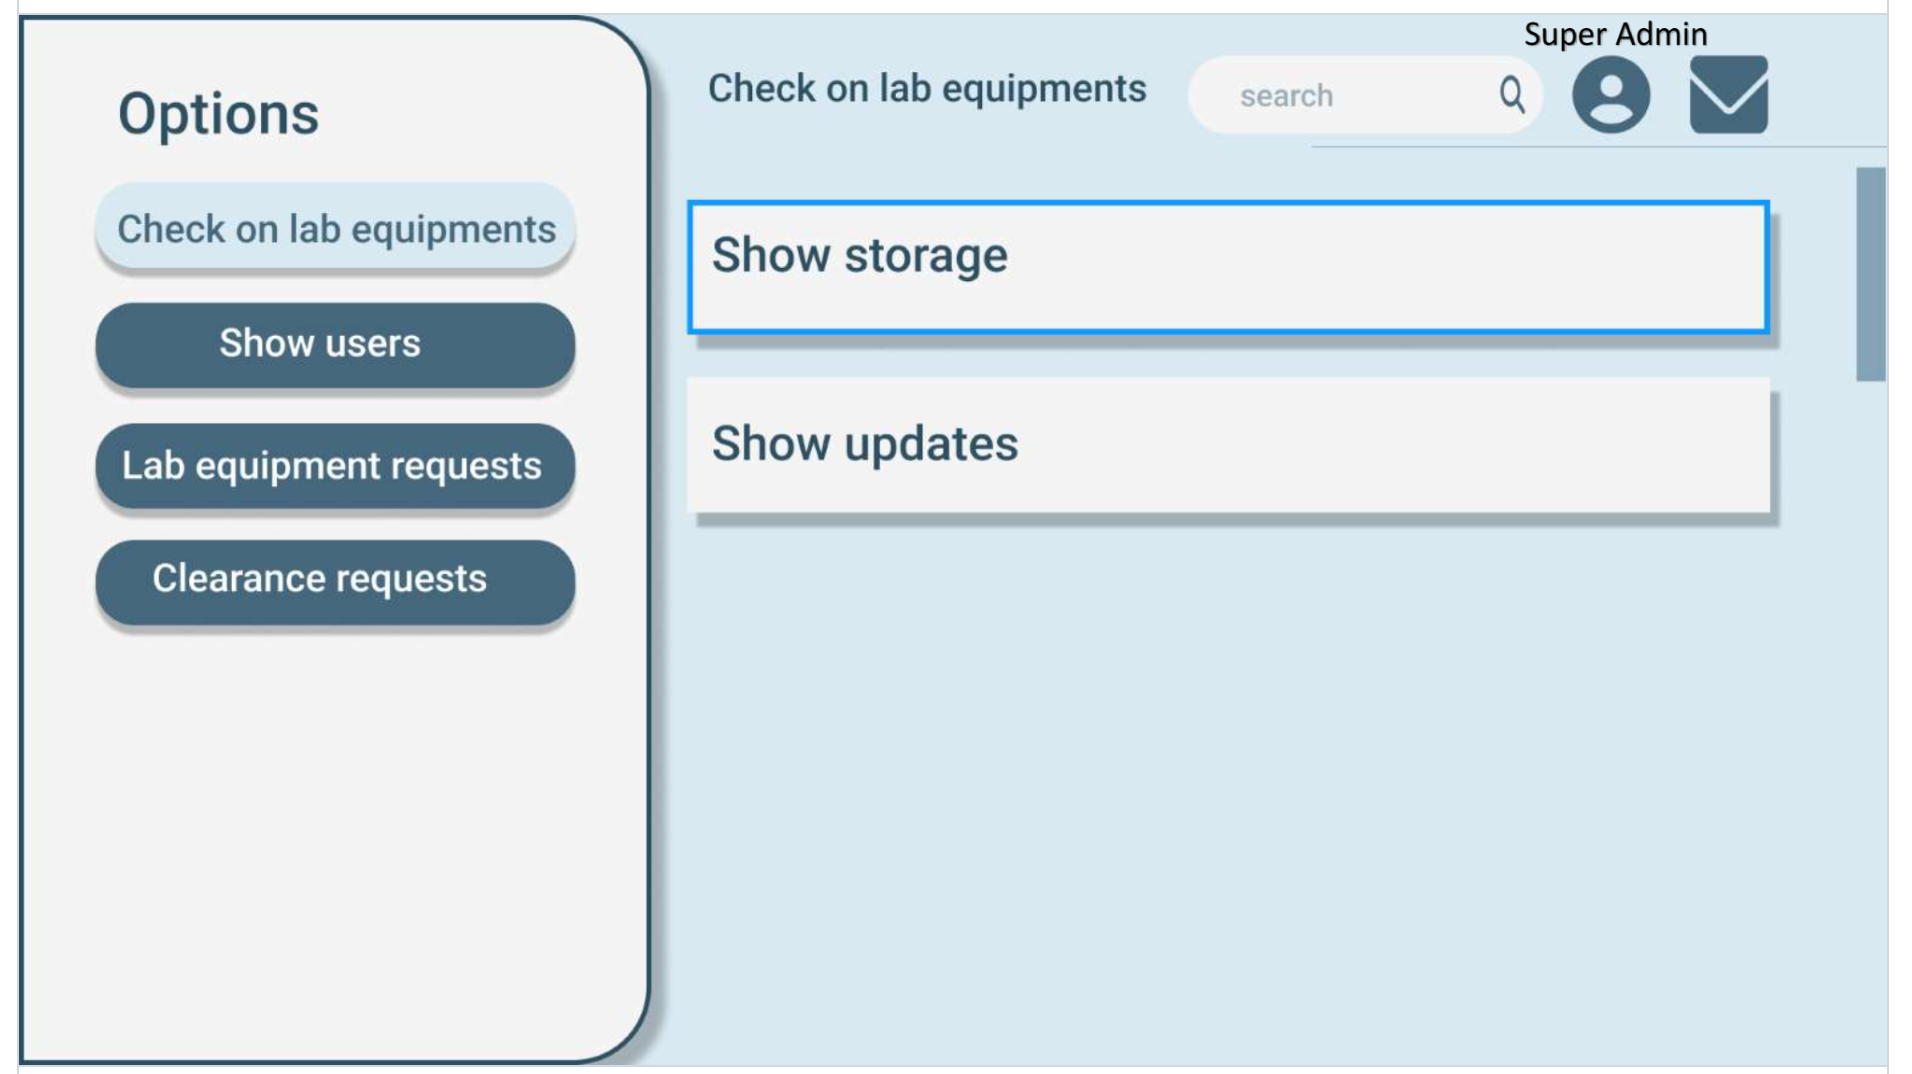
\includegraphics[width= 0.5\textwidth , height= 0.3\paperheight]{SuperAdminInventoryCheck1.png}
            \caption{Inventory Checking Page}
        \label{fig:63}
        
    \end{figure}

    

    \begin{figure}

        \centering

        \begin{minipage}[b]{0.45\textwidth}
            \centering
            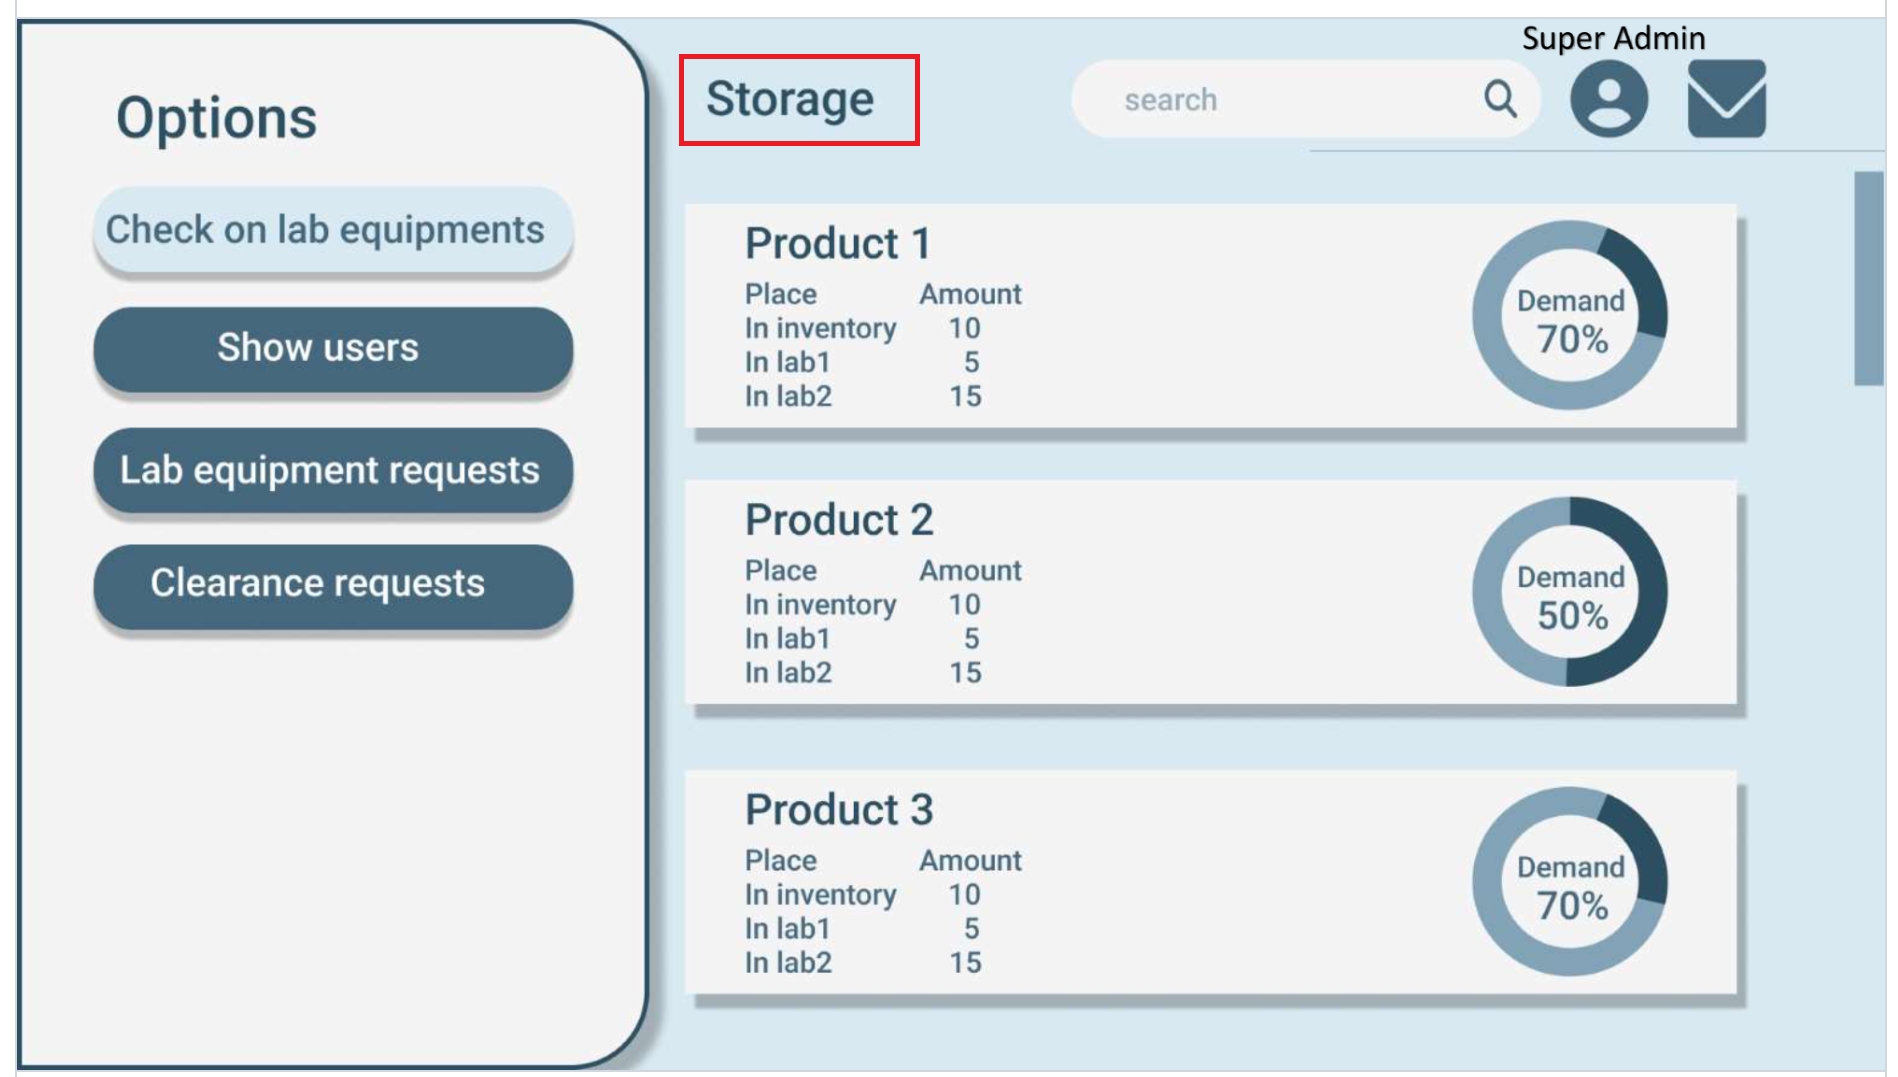
\includegraphics[width= \textwidth , height= 0.2\paperheight]{SuperAdminInventoryCheck2.png}
            \caption{View Stock Storage}
            \label{fig:64}
        \end{minipage}
        \begin{minipage}[b]{0.45\textwidth}
            \centering
            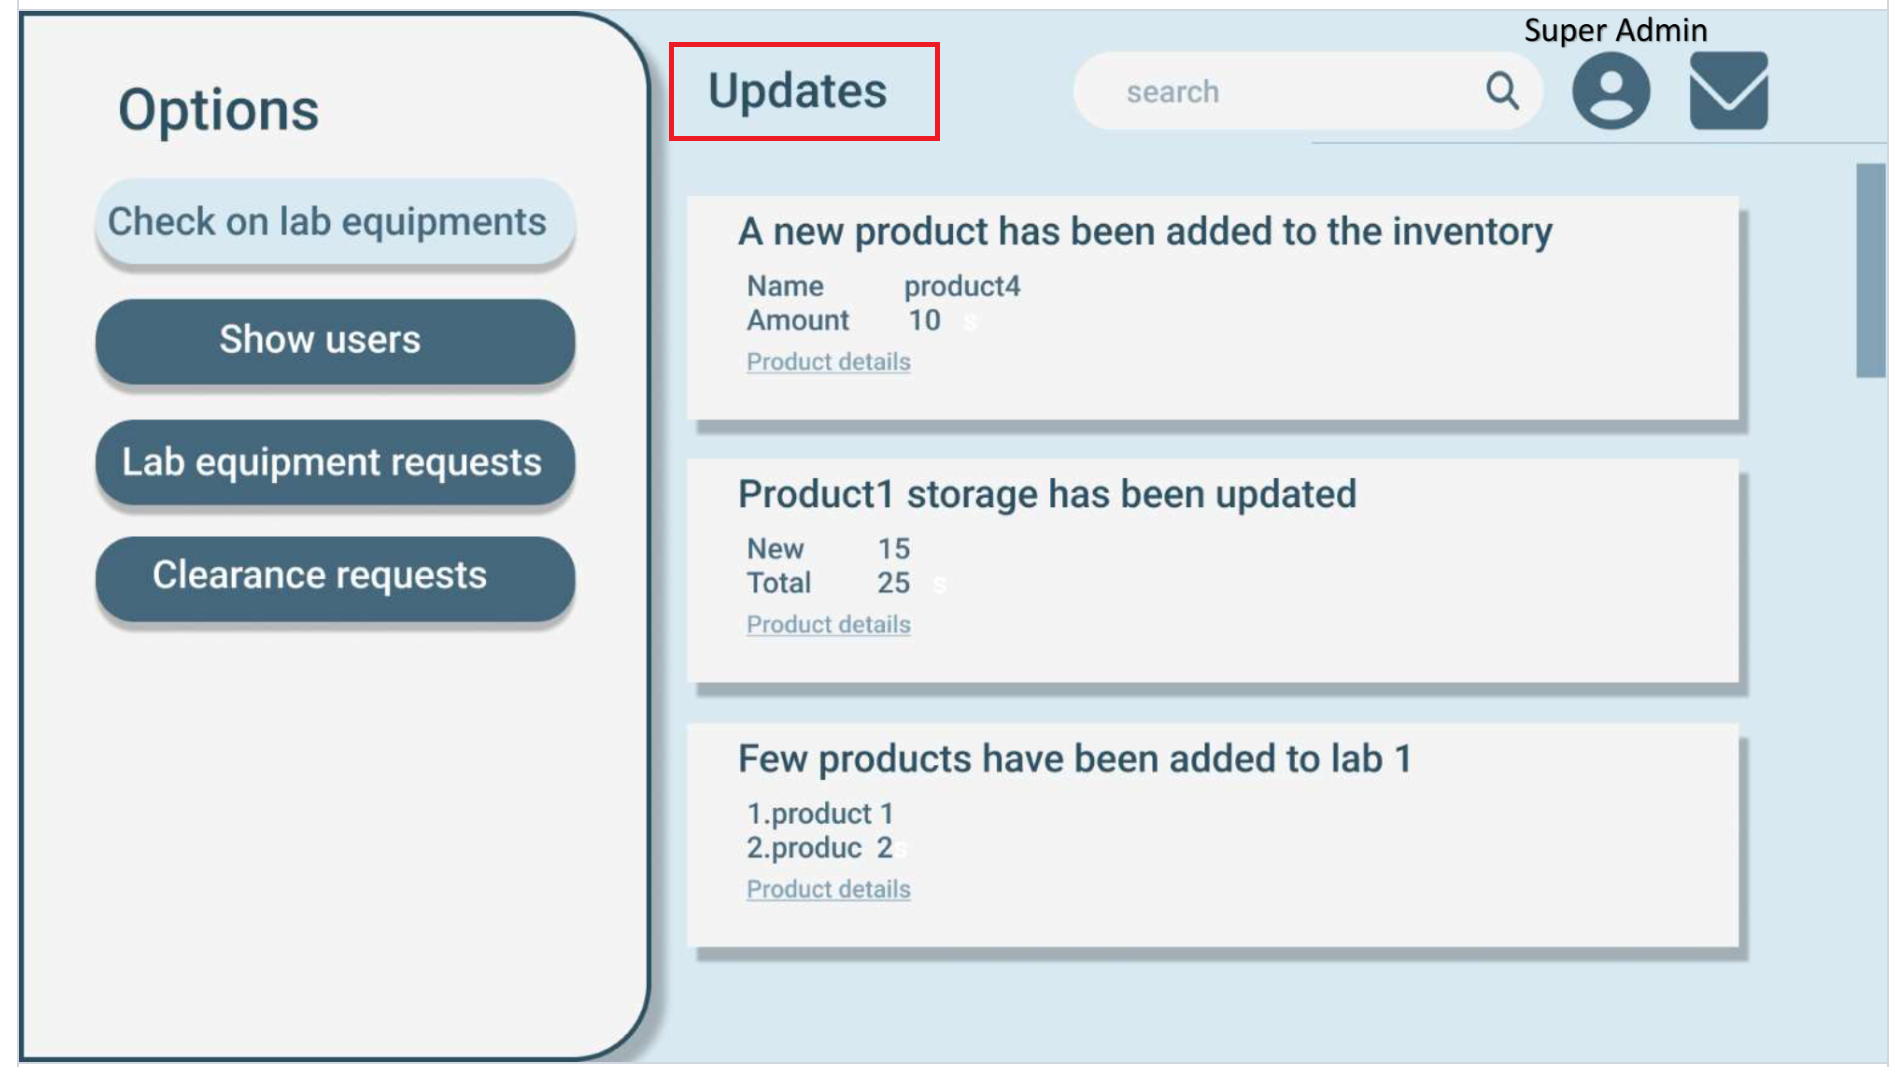
\includegraphics[width= \textwidth , height= 0.2\paperheight]{SuperAdminInventoryCheck3.png}
            \caption{View Stock Updates}
            \label{fig:65}

        \end{minipage}
        
    \end{figure}

\end{frame}

\begin{frame}{The User viewing Page}

     \begin{figure}
        \centering
        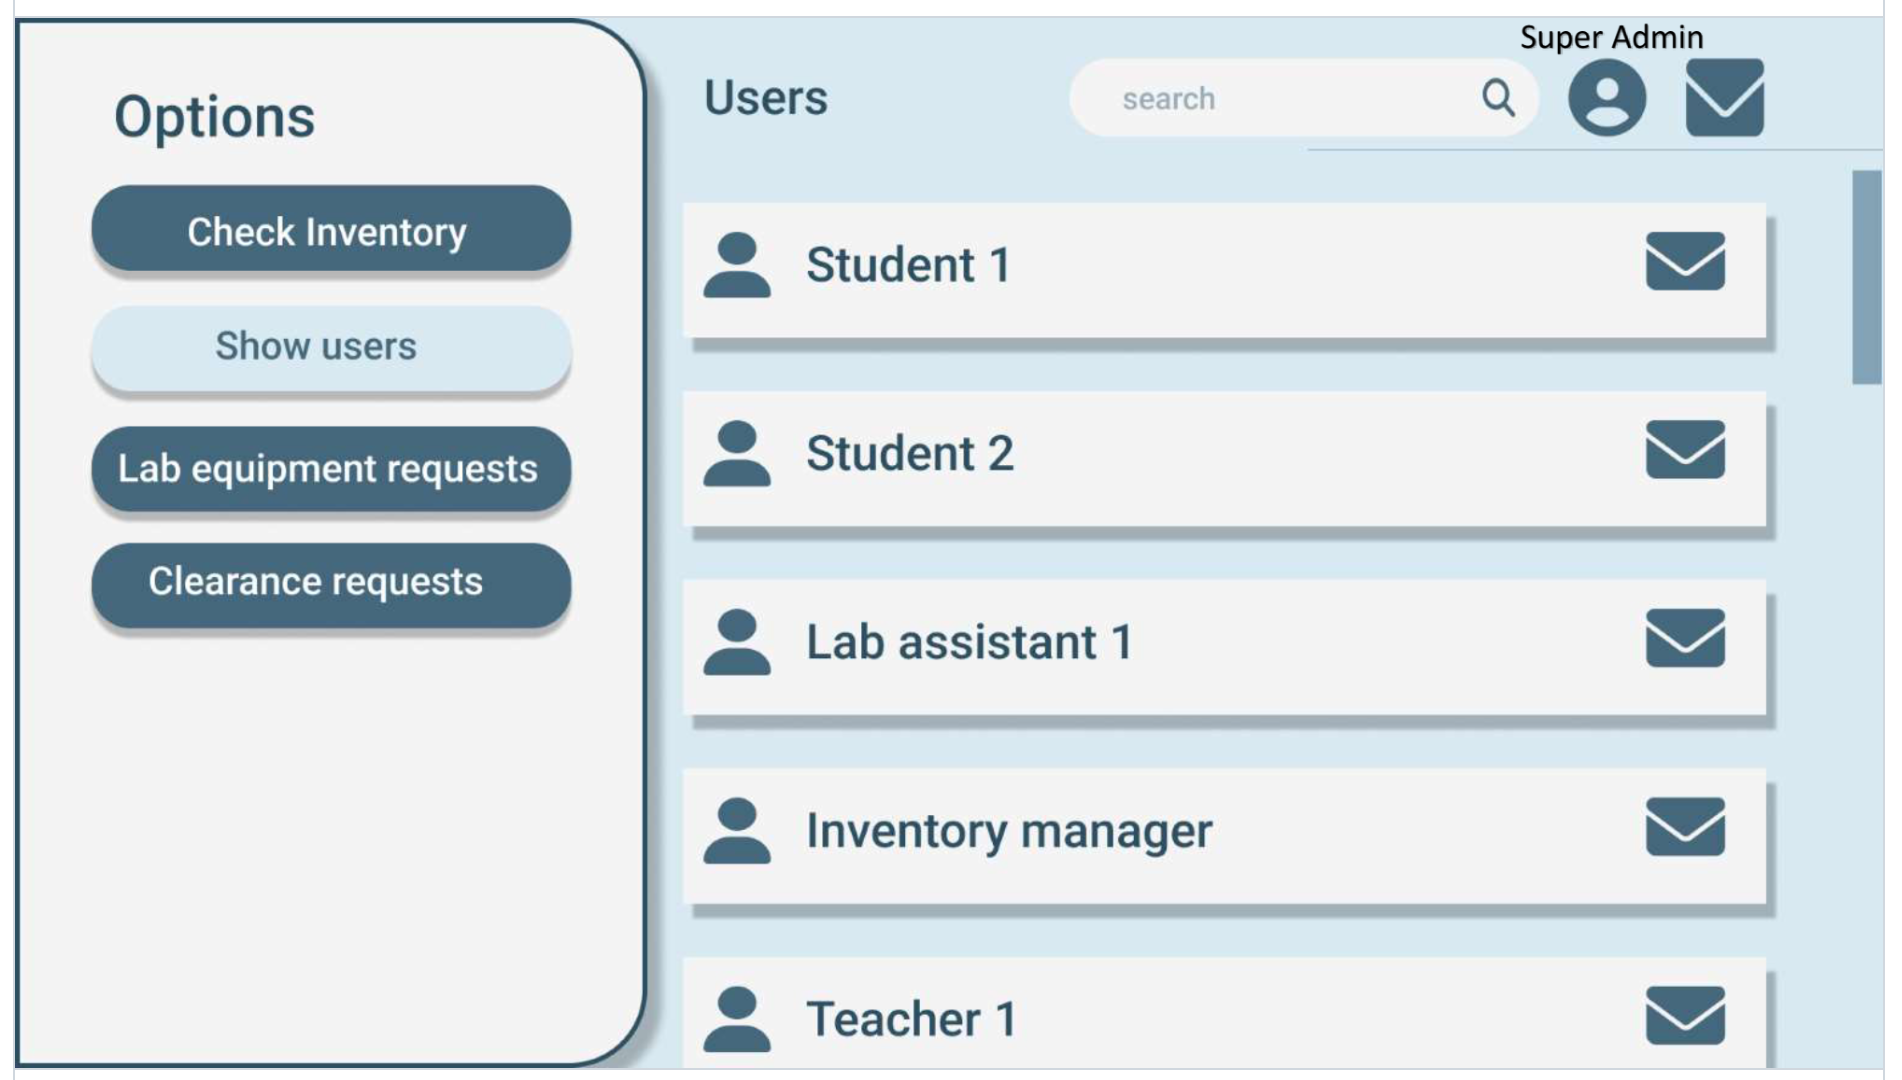
\includegraphics[width= 0.9\textwidth , height= 0.5\paperheight]{SuperAdminShowUser.png}
        \caption{Page for showing Userlist}
        \label{fig:66}
    \end{figure}

\end{frame}

\begin{frame}{The Clearance Approval Page}

     \begin{figure}
        \centering
        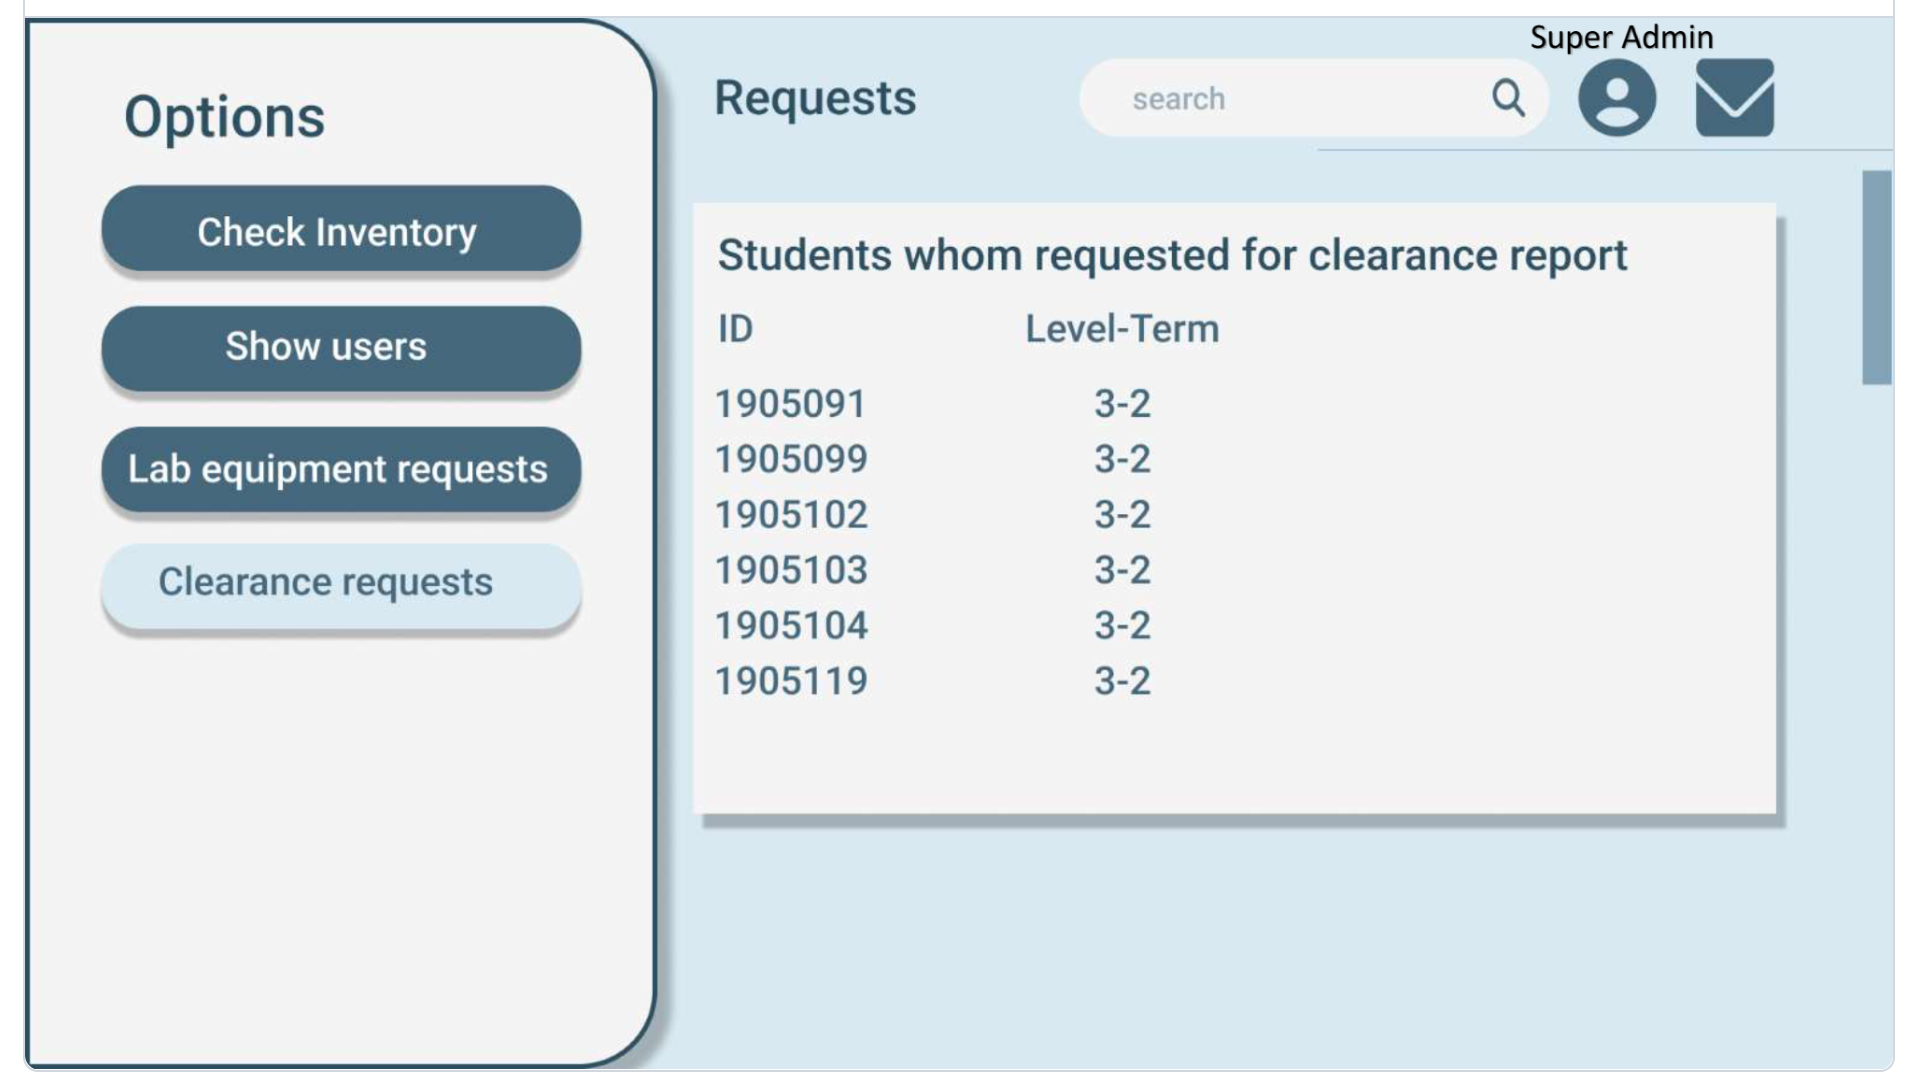
\includegraphics[width= 0.9\textwidth , height= 0.5\paperheight]{SuperAdminGiveClearance.png}
        \caption{Page for approving clearance}
        \label{fig:67}
    \end{figure}

\end{frame}

\section{Entity Relationship Diagram(ERD)}

\begin{frame}{Entity Relationship Diagram(ERD)}

     \begin{figure}
        \centering
        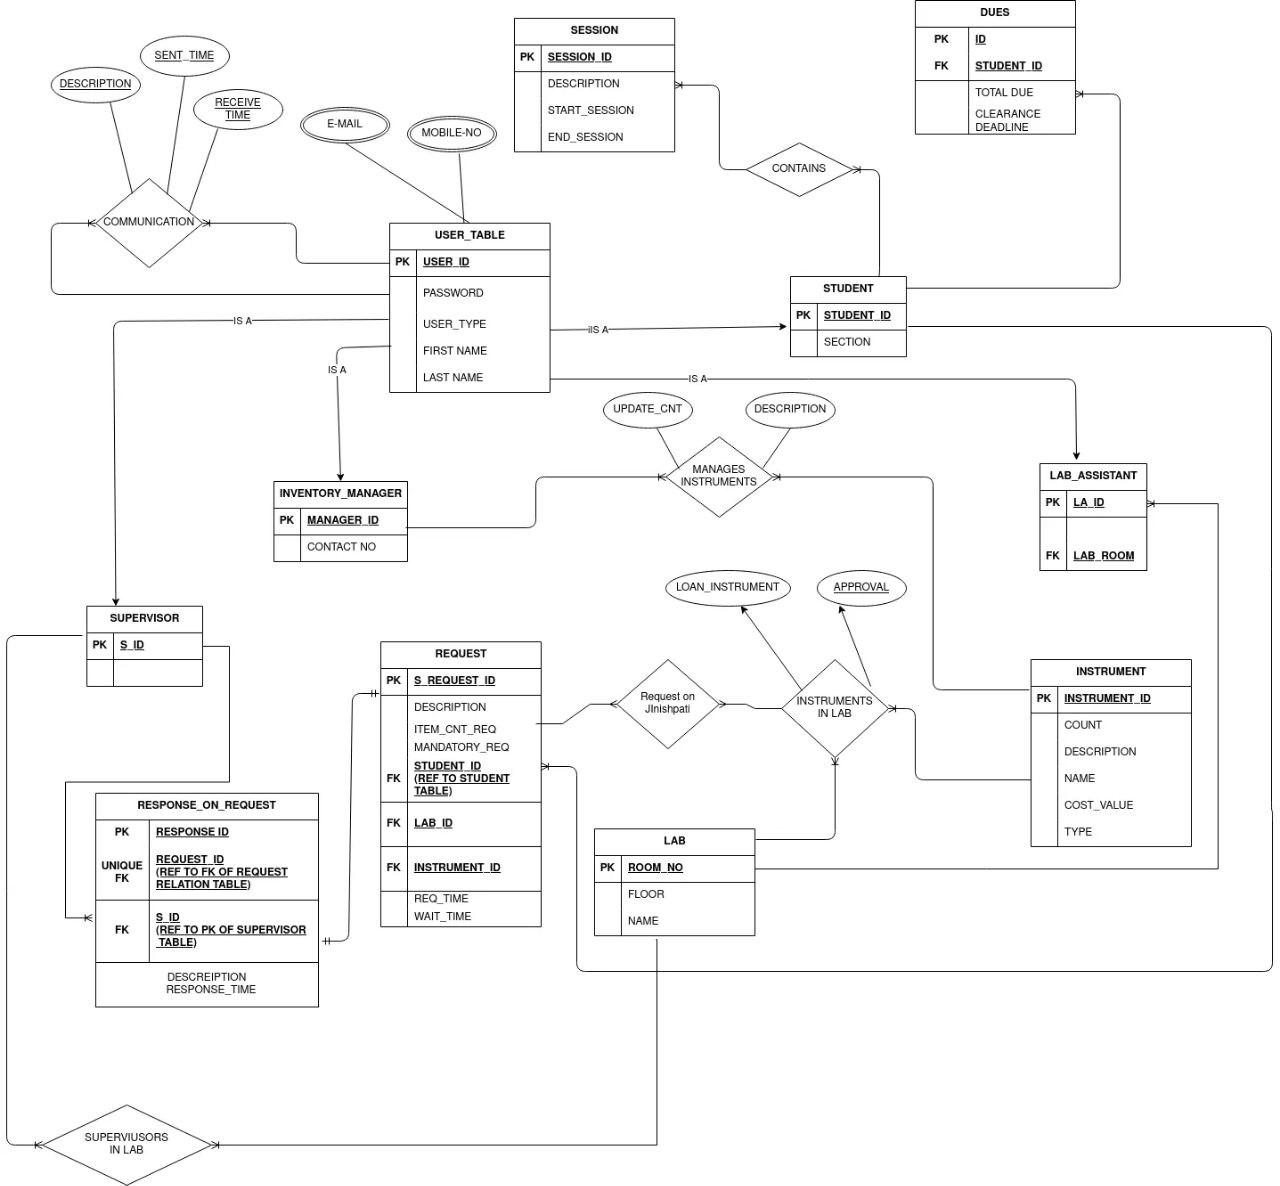
\includegraphics[width= 0.9\textwidth , height= 0.8\paperheight]{ERD.jpg}
        \caption{{Entity Relationship Diagram}}
        \label{fig:4}
    \end{figure}

\end{frame}

\section{Unified Modeling Language(UML) Class Diagram}

\begin{frame}{Login Class Diagram}

     \begin{figure}
        \centering
        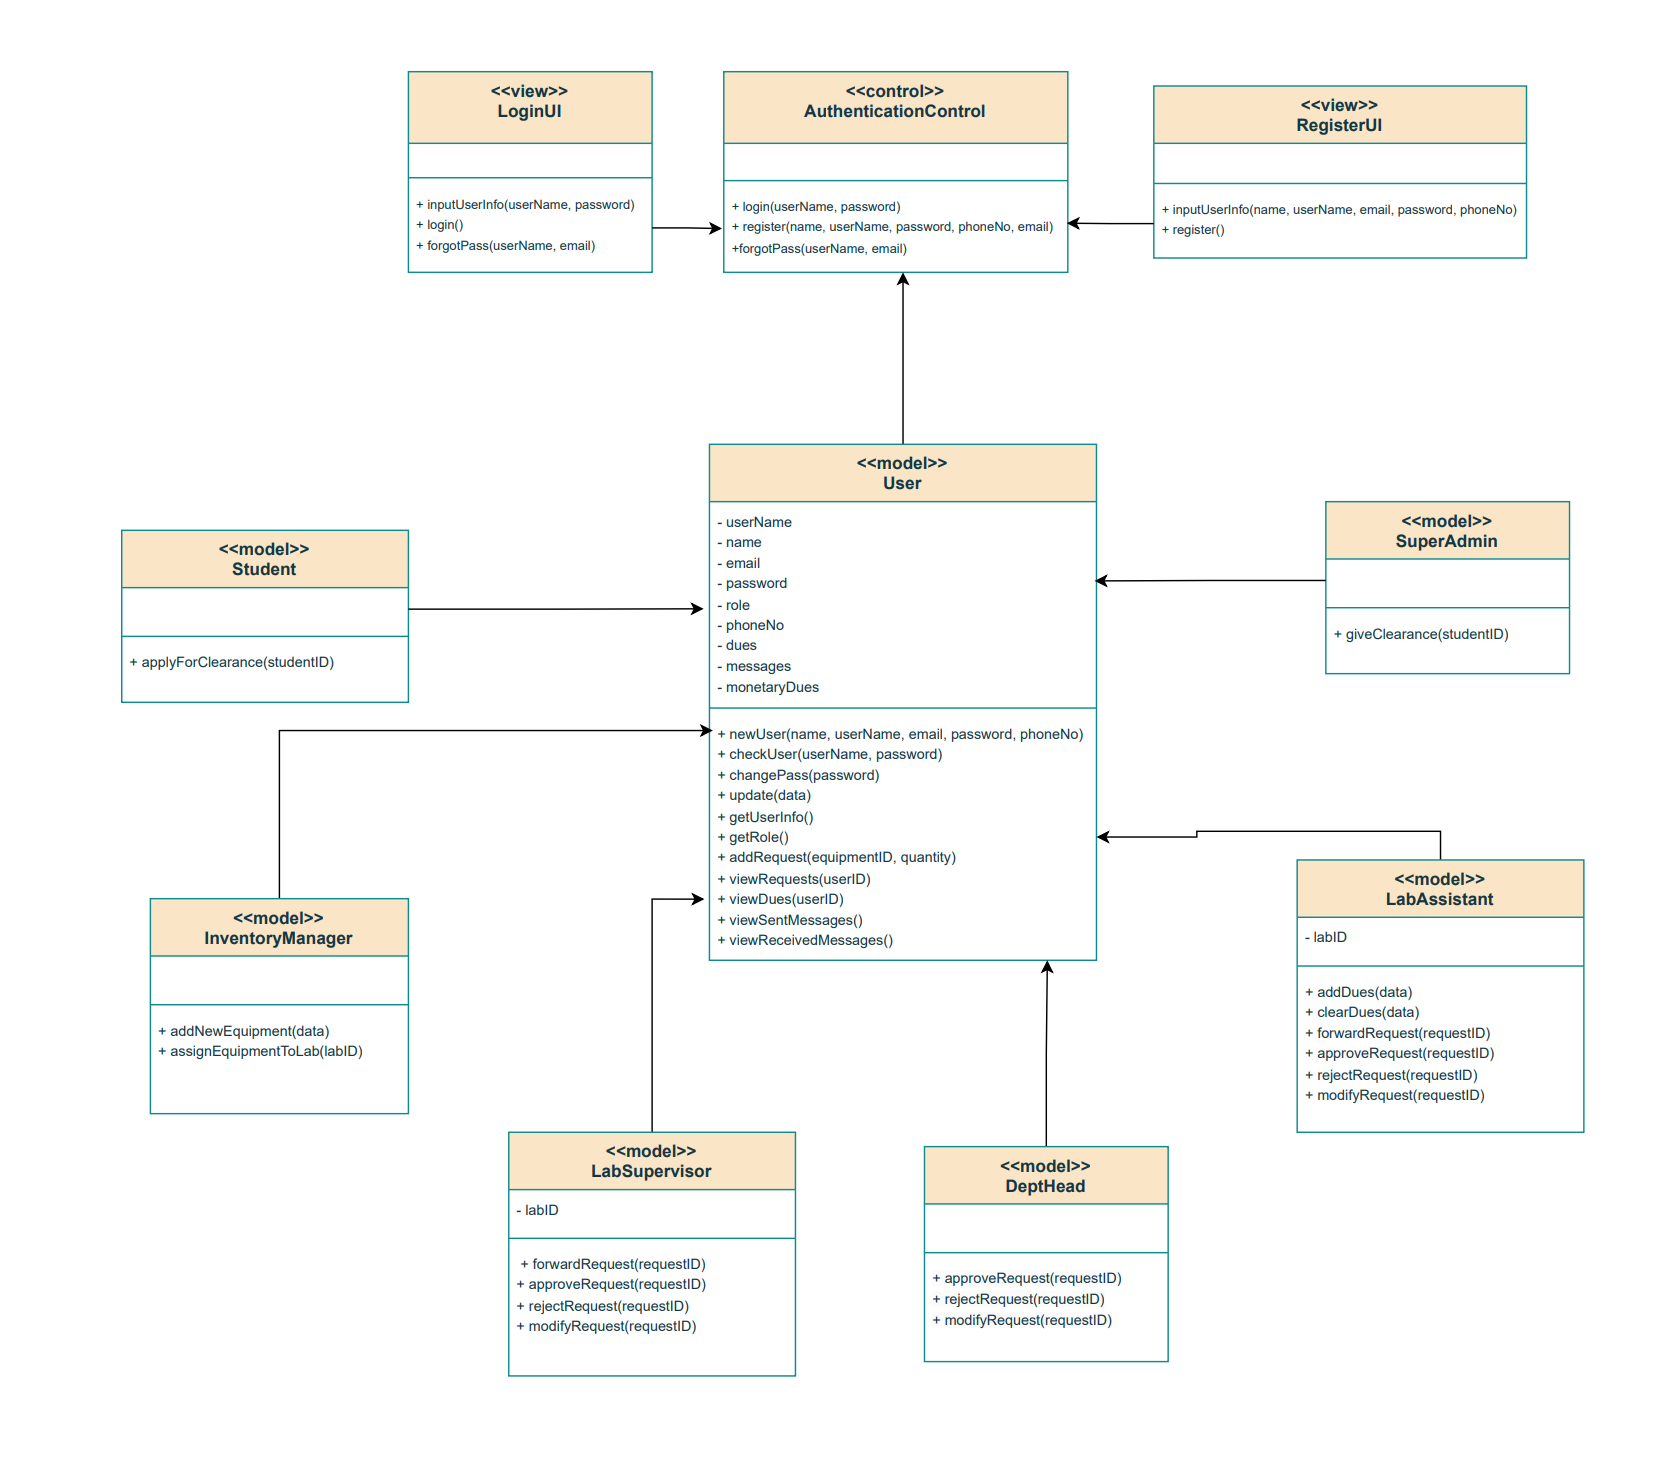
\includegraphics[width= 0.9\textwidth , height= 0.8\paperheight]{LoginUML.png}
        \caption{{Login}}
        \label{fig:5}
    \end{figure}

\end{frame}

\begin{frame}{Home Page Class Diagram}

     \begin{figure}
        \centering
        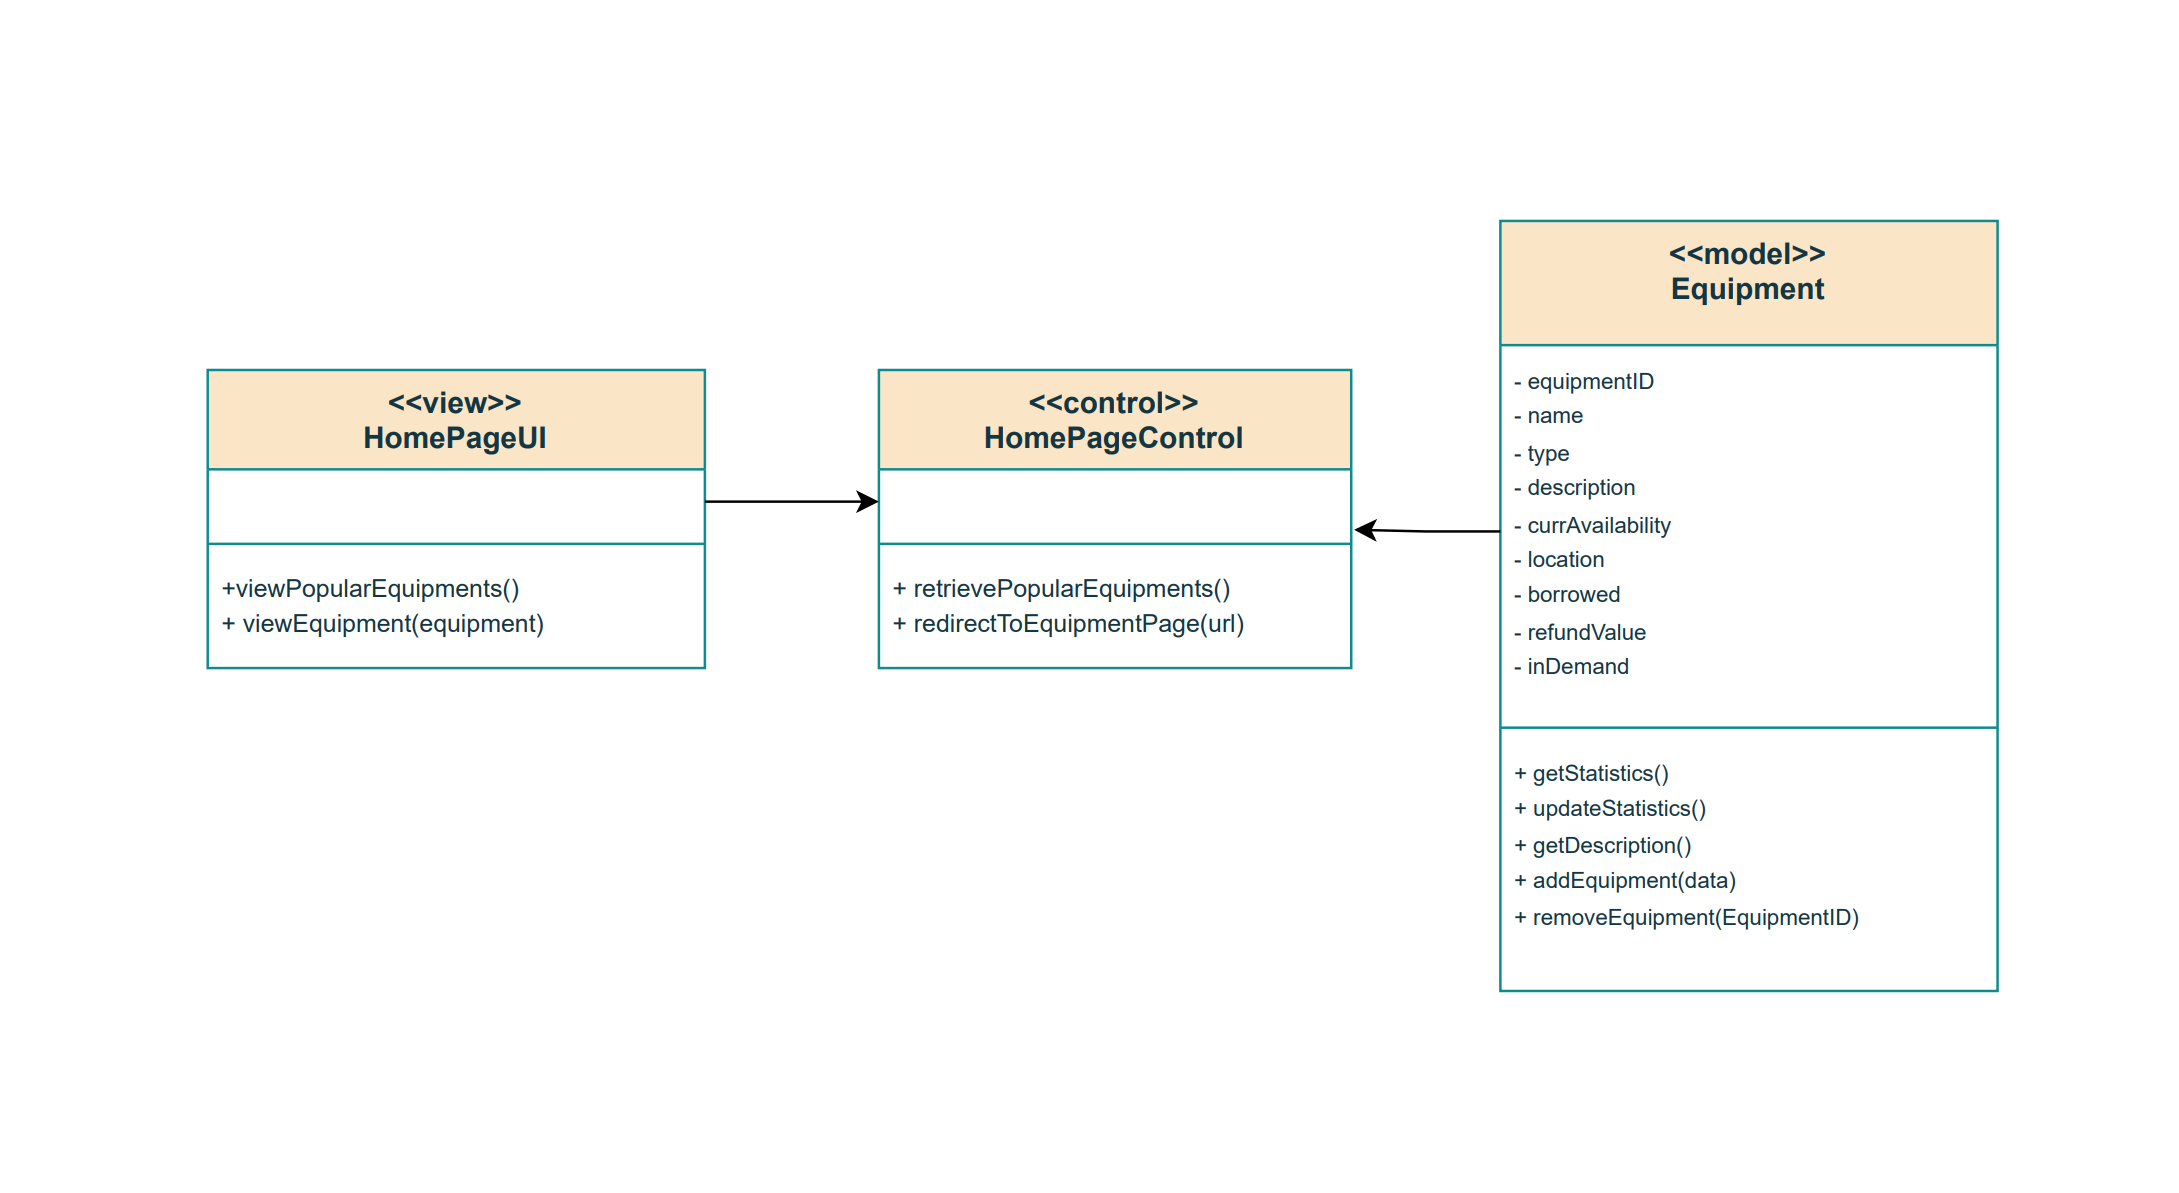
\includegraphics[width= 0.9\textwidth , height= 0.8\paperheight]{HomePageUML.png}
        \caption{{Home Page}}
        \label{fig:6}
    \end{figure}

\end{frame}

\begin{frame}{Search Equipment Class Diagram}

     \begin{figure}
        \centering
        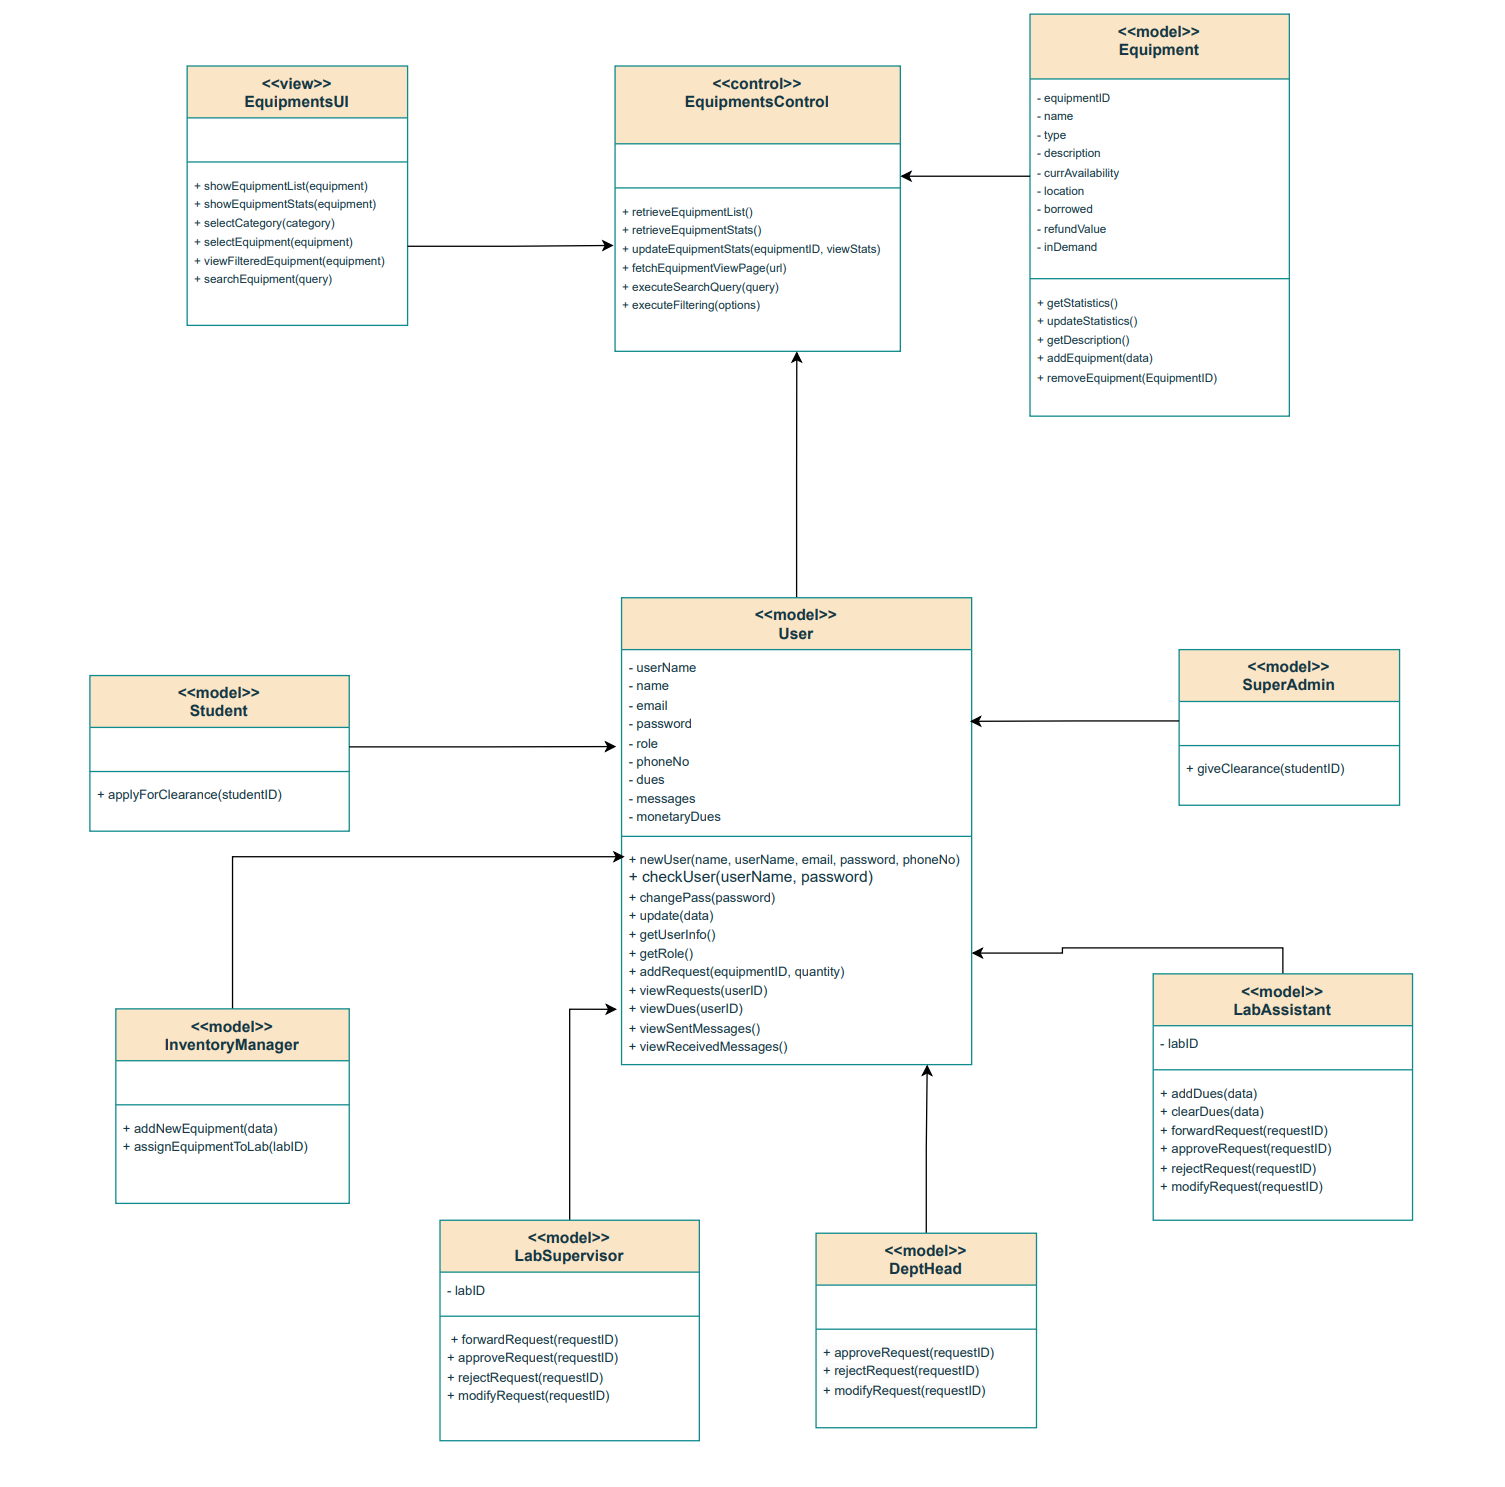
\includegraphics[width= 0.9\textwidth , height= 0.8\paperheight]{EquipmentSearchUML.png}
        \caption{{Search Equipments}}
        \label{fig:7}
    \end{figure}

\end{frame}

\begin{frame}{Individual Equipment Class Diagram}

     \begin{figure}
        \centering
        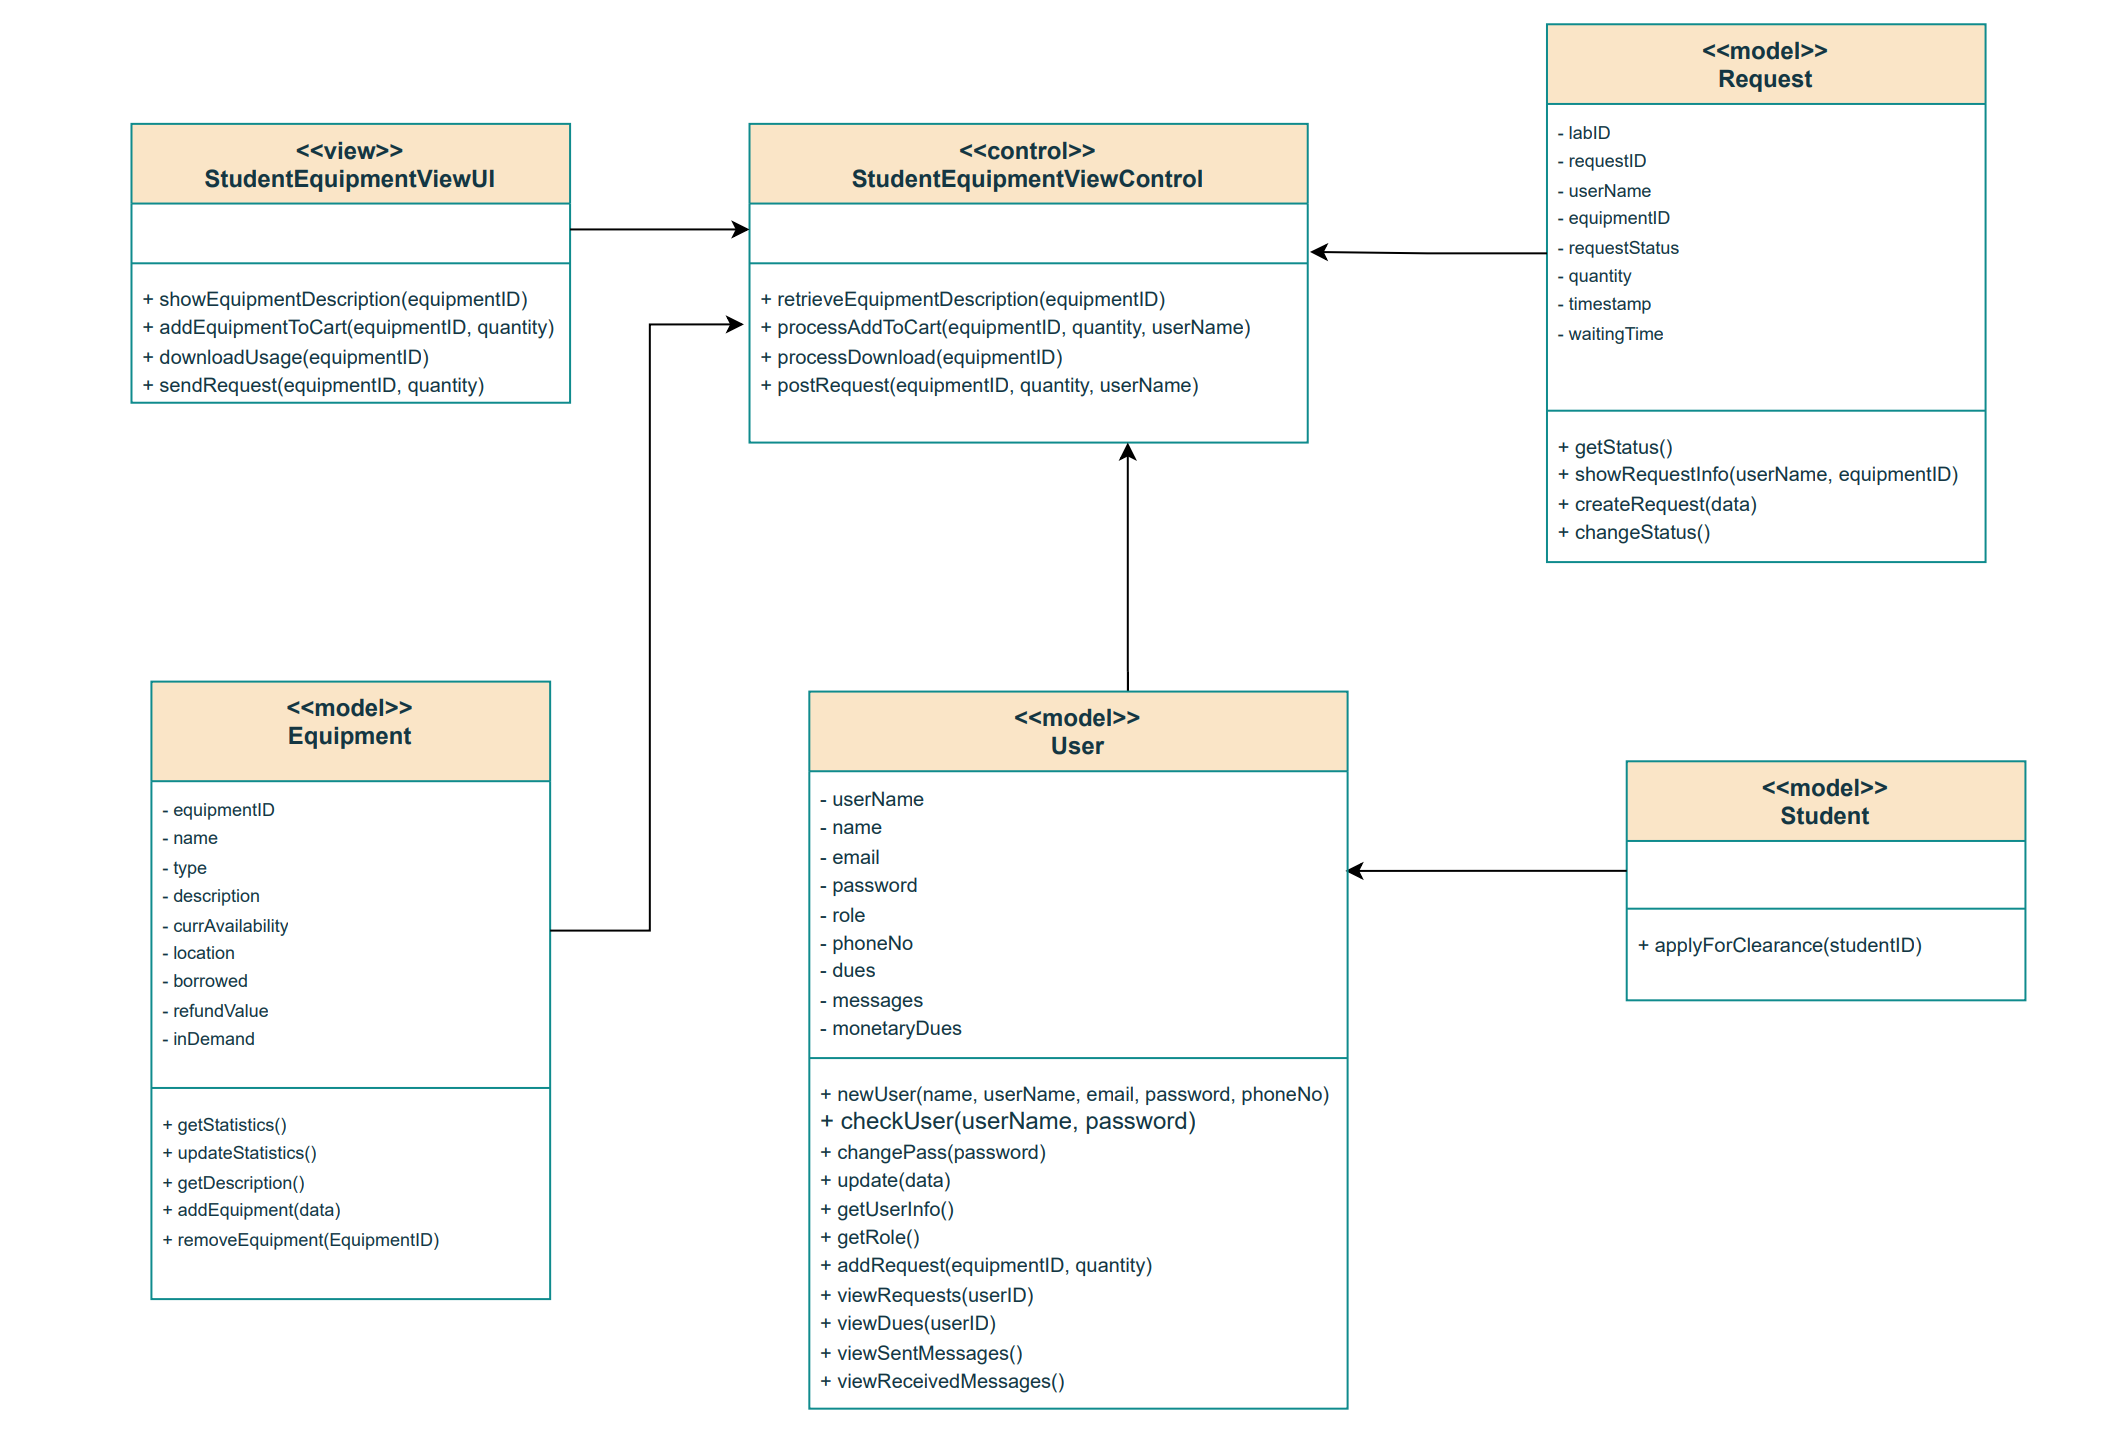
\includegraphics[width= 0.9\textwidth , height= 0.8\paperheight]{IndividualEquipmentUML.png}
        \caption{{Individual Equipments}}
        \label{fig:8}
    \end{figure}

\end{frame}

\begin{frame}{Add Equipment Class Diagram}

     \begin{figure}
        \centering
        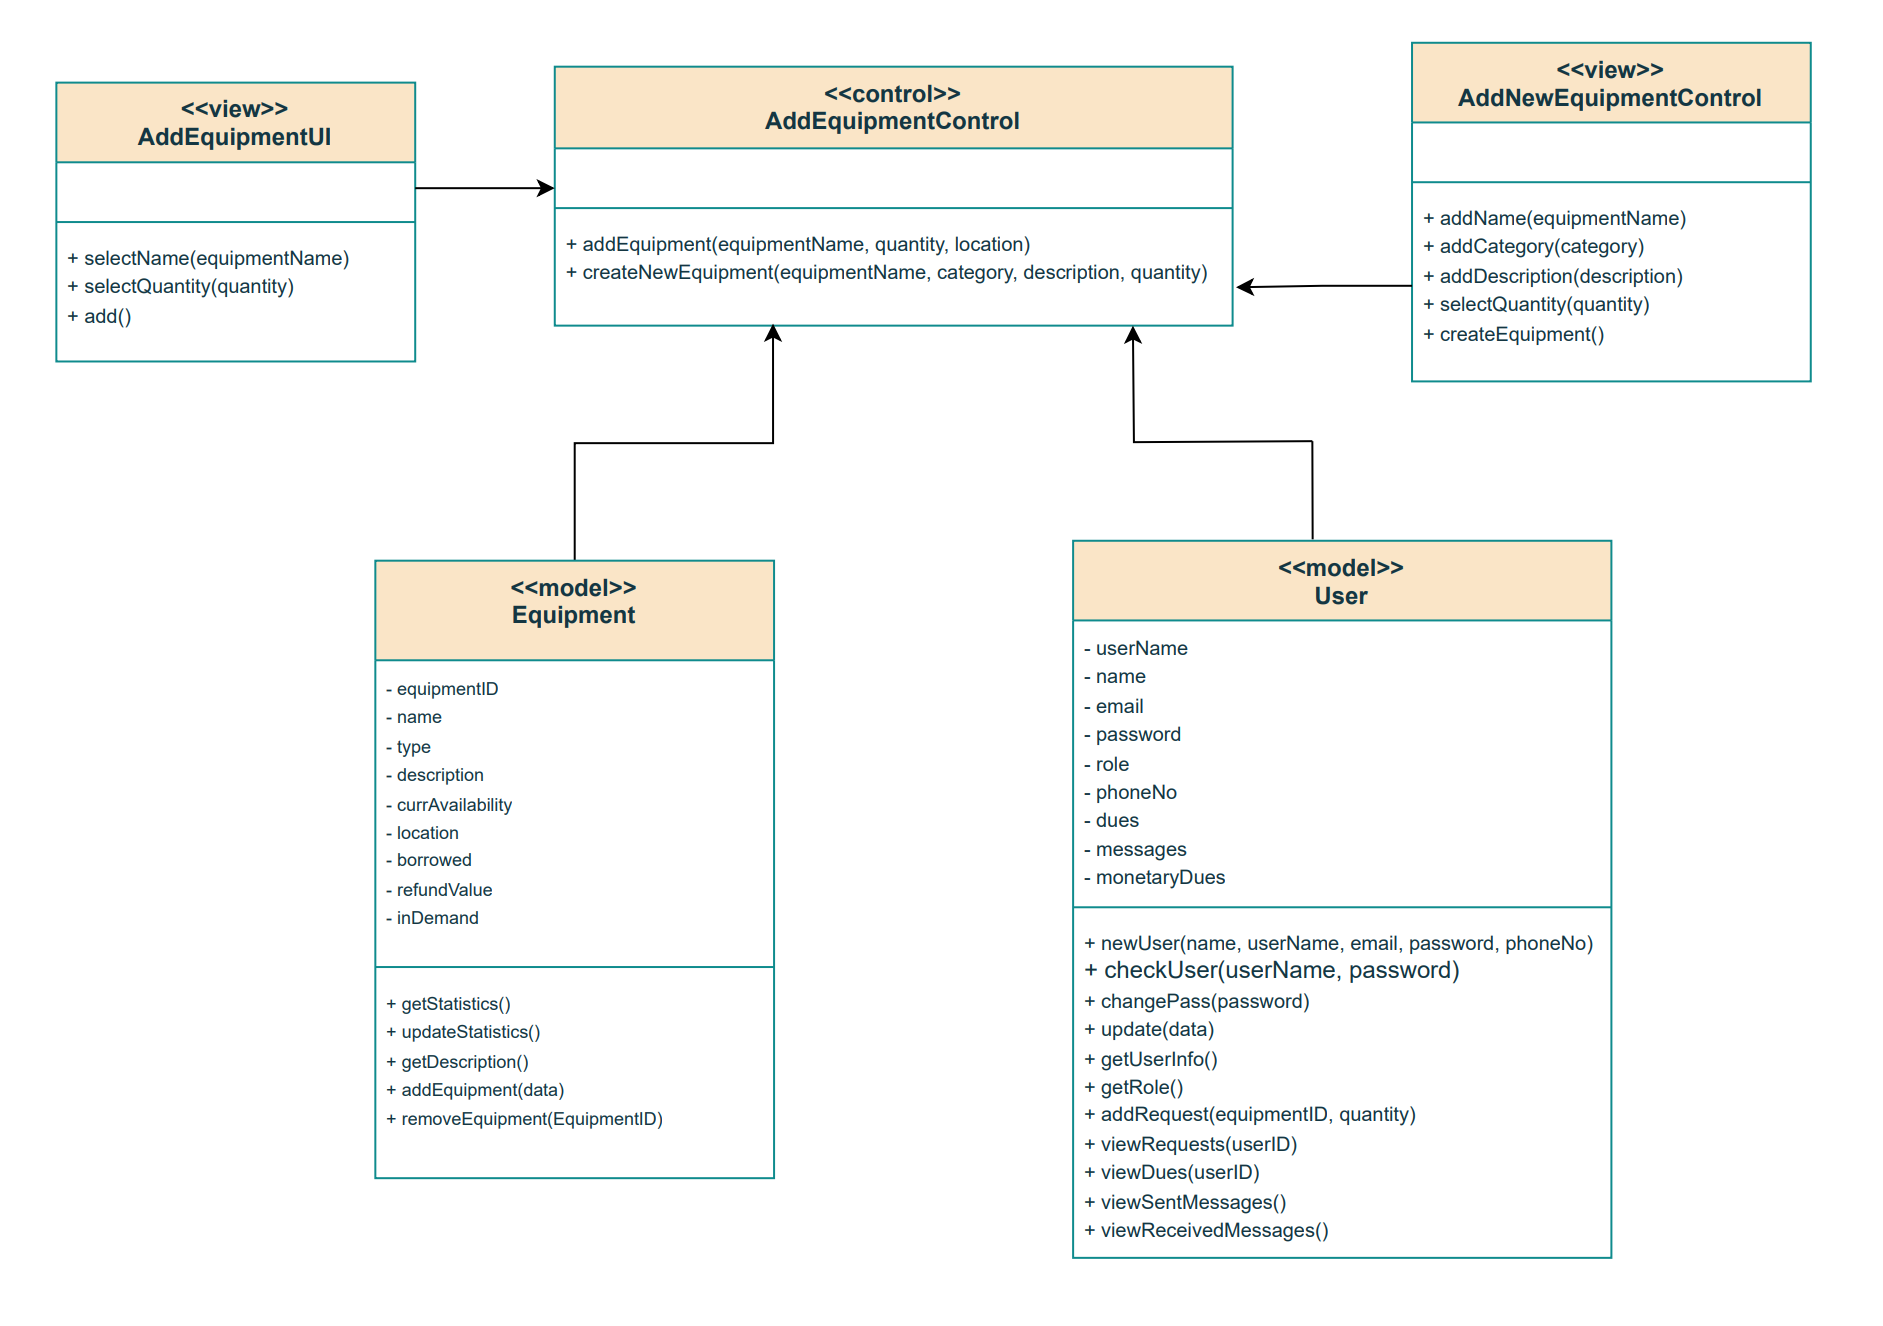
\includegraphics[width= 0.9\textwidth , height= 0.8\paperheight]{AddEquipmentsUML.png}
        \caption{{Add Equipments}}
        \label{fig:9}
    \end{figure}

\end{frame}

\begin{frame}{Respond on Request Class Diagram}

     \begin{figure}
        \centering
        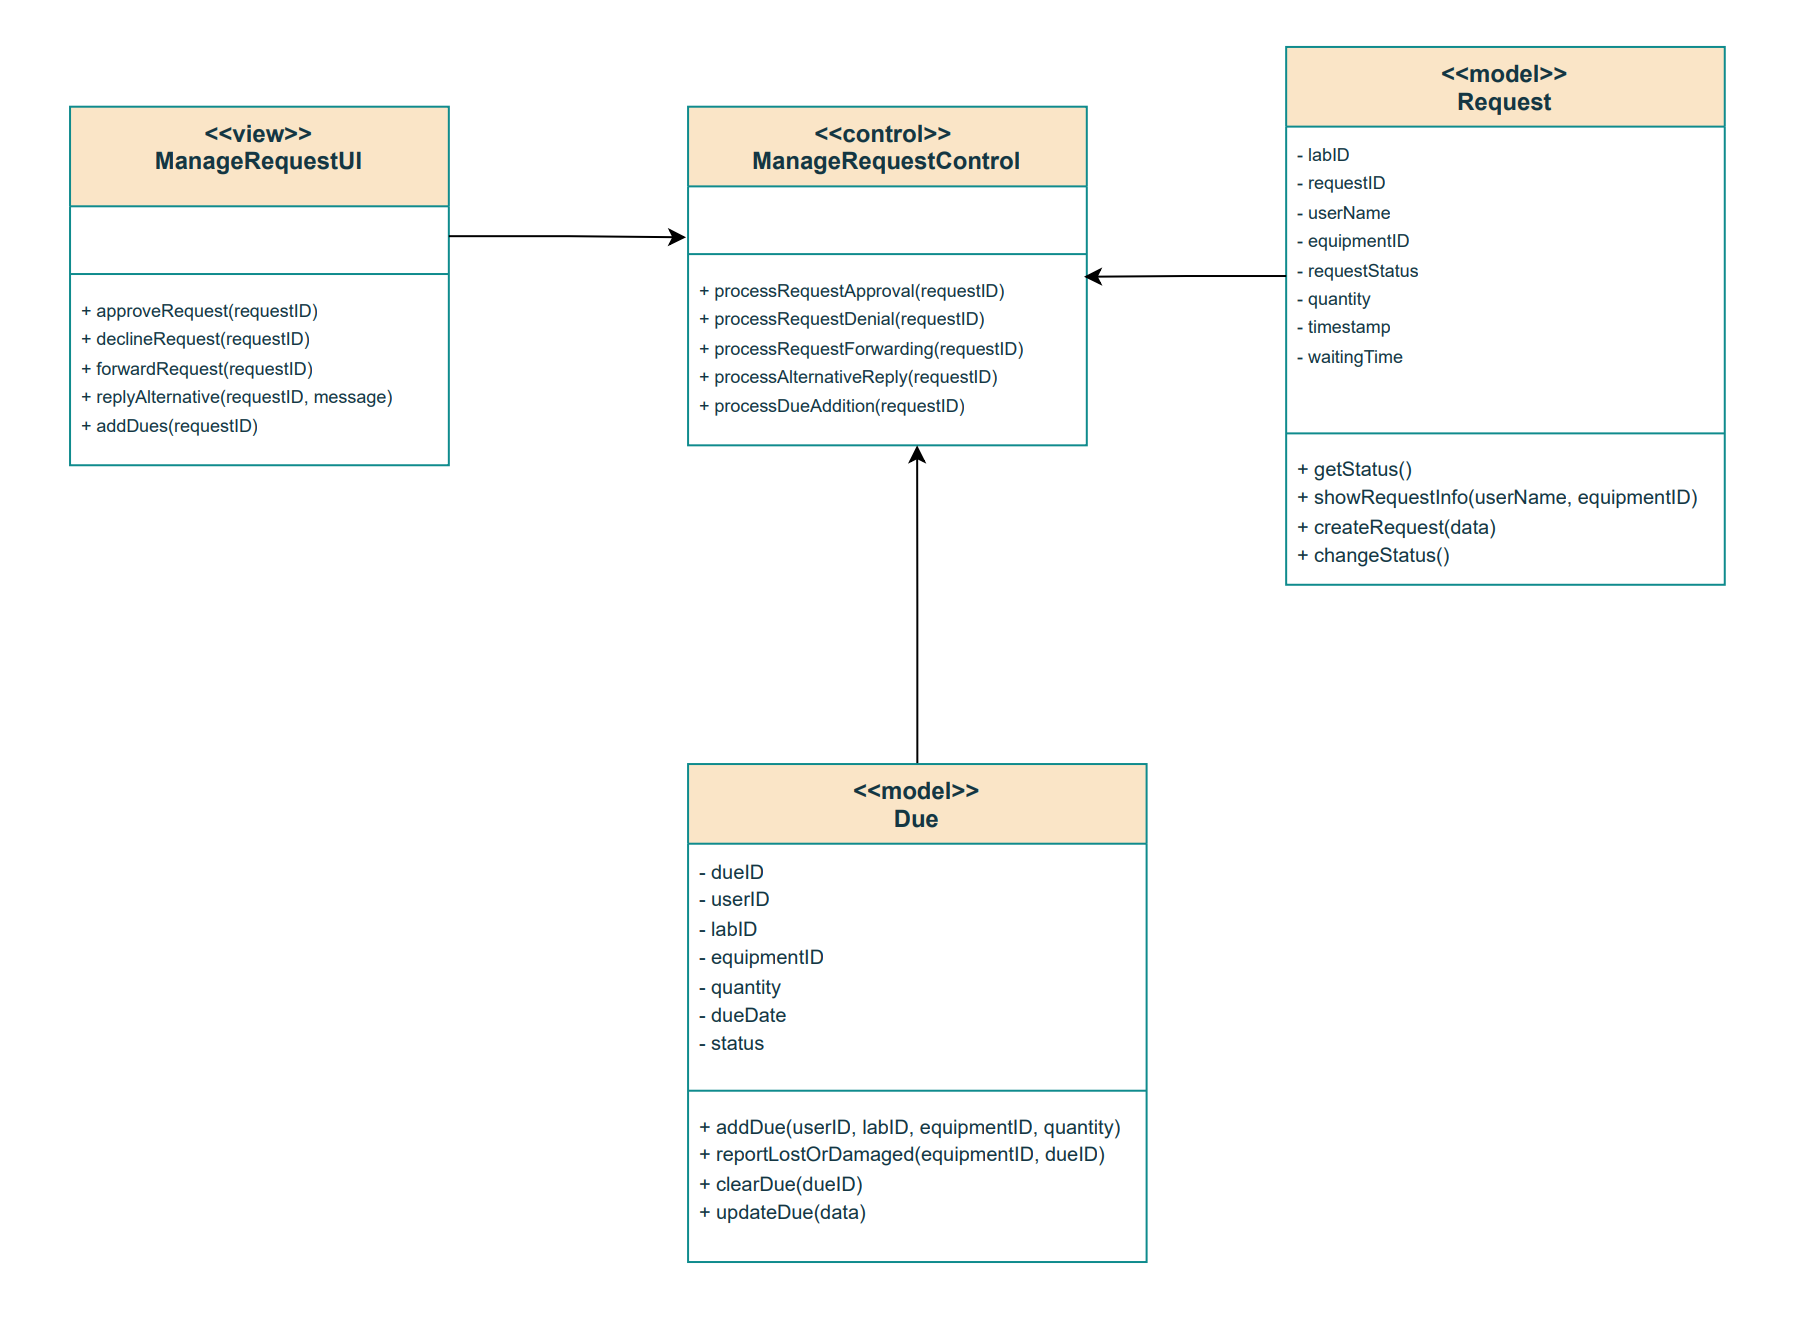
\includegraphics[width= 0.9\textwidth , height= 0.8\paperheight]{ResponseRequestsUML.png}
        \caption{{Response on Request}}
        \label{fig:10}
    \end{figure}

\end{frame}

\begin{frame}{Apply Clearance Class Diagram}

     \begin{figure}
        \centering
        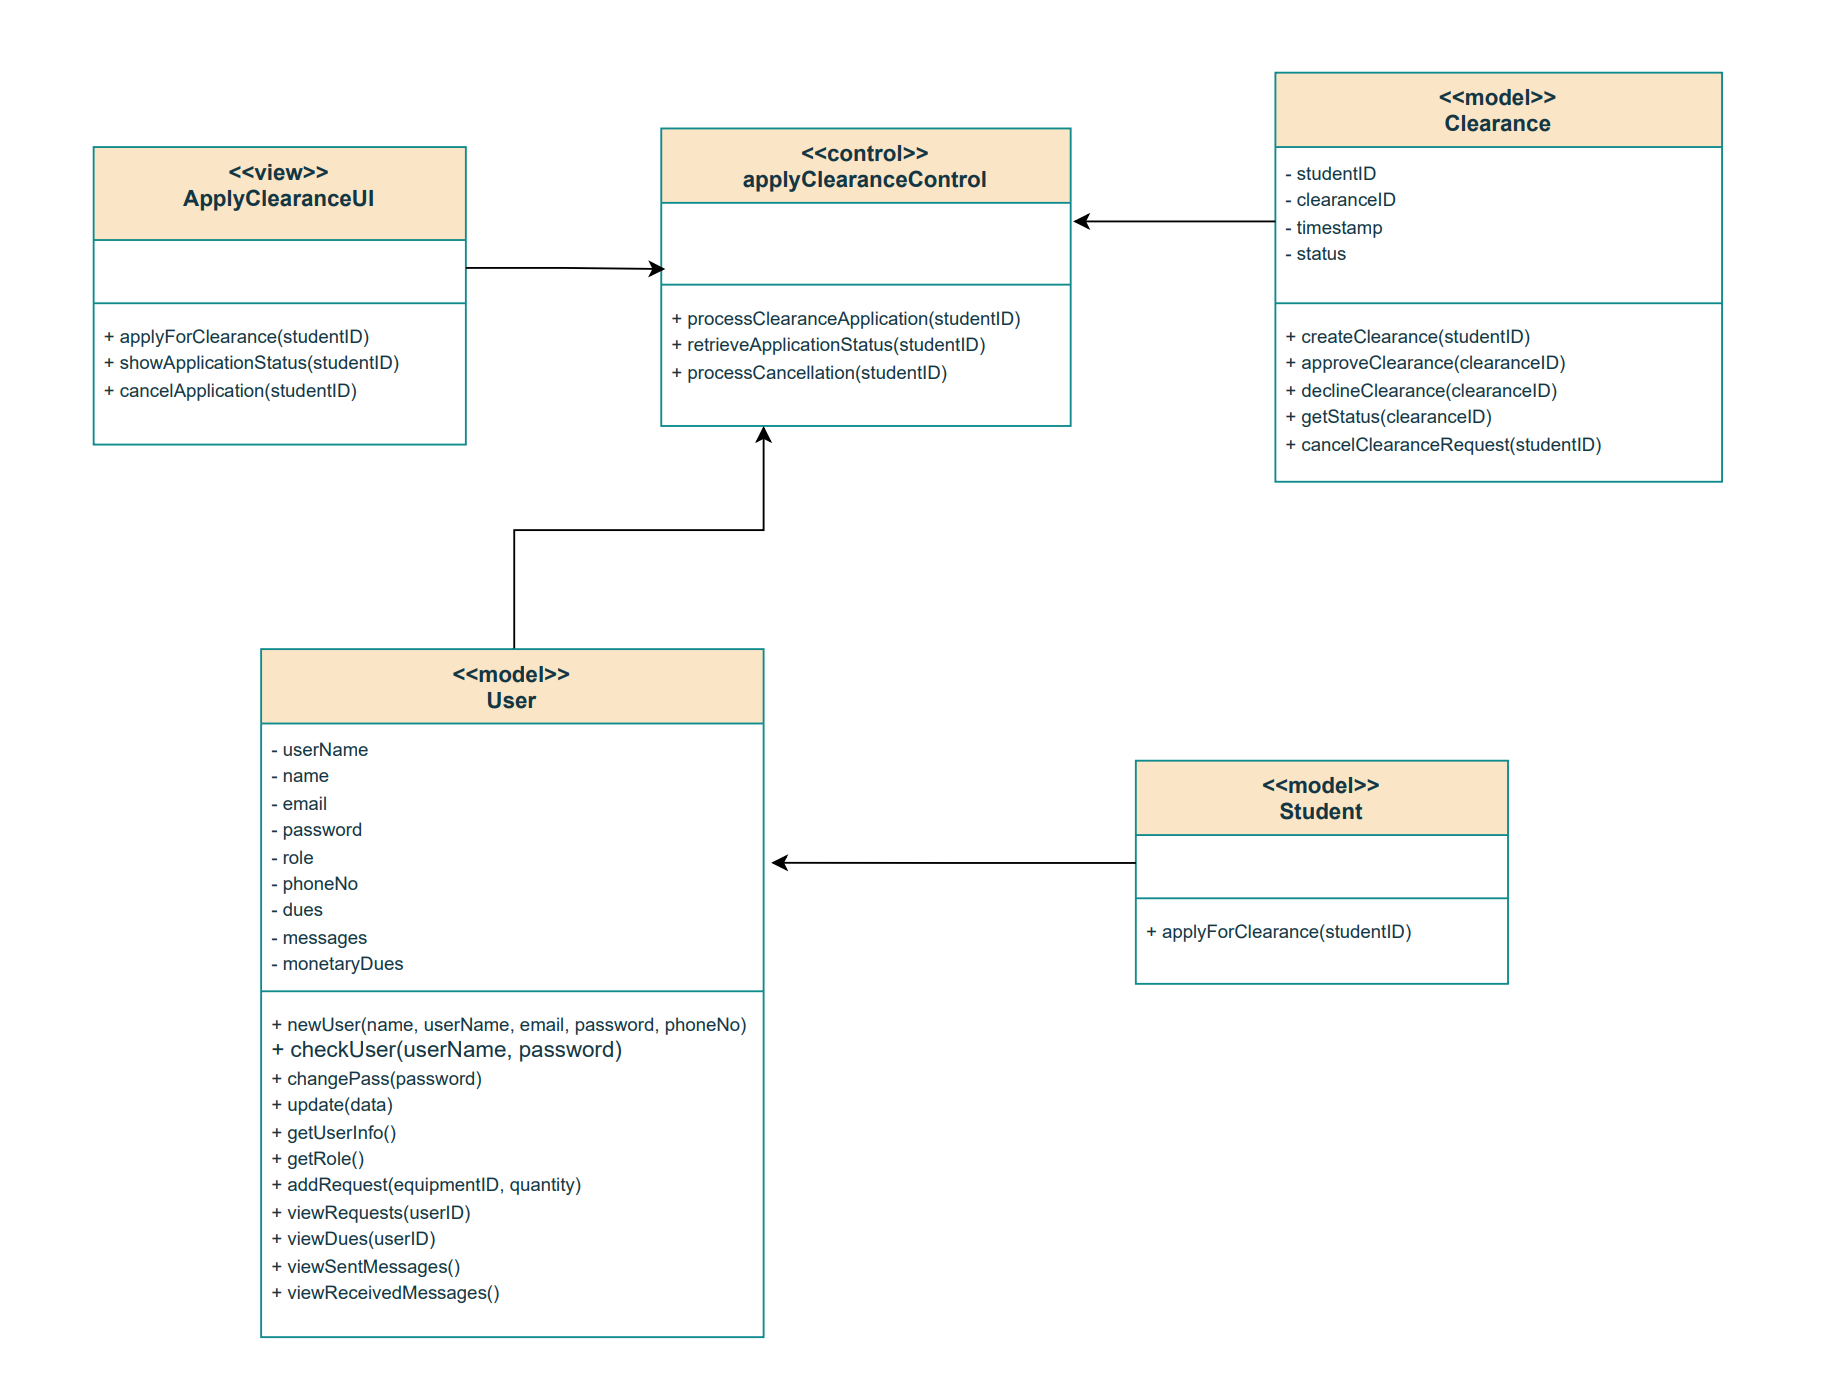
\includegraphics[width= 0.9\textwidth , height= 0.8\paperheight]{ApplyClearanceUML.png}
        \caption{{Apply Clearance}}
        \label{fig:11}
    \end{figure}

\end{frame}

\begin{frame}{Respond on Clearance Request Class Diagram}

     \begin{figure}
        \centering
        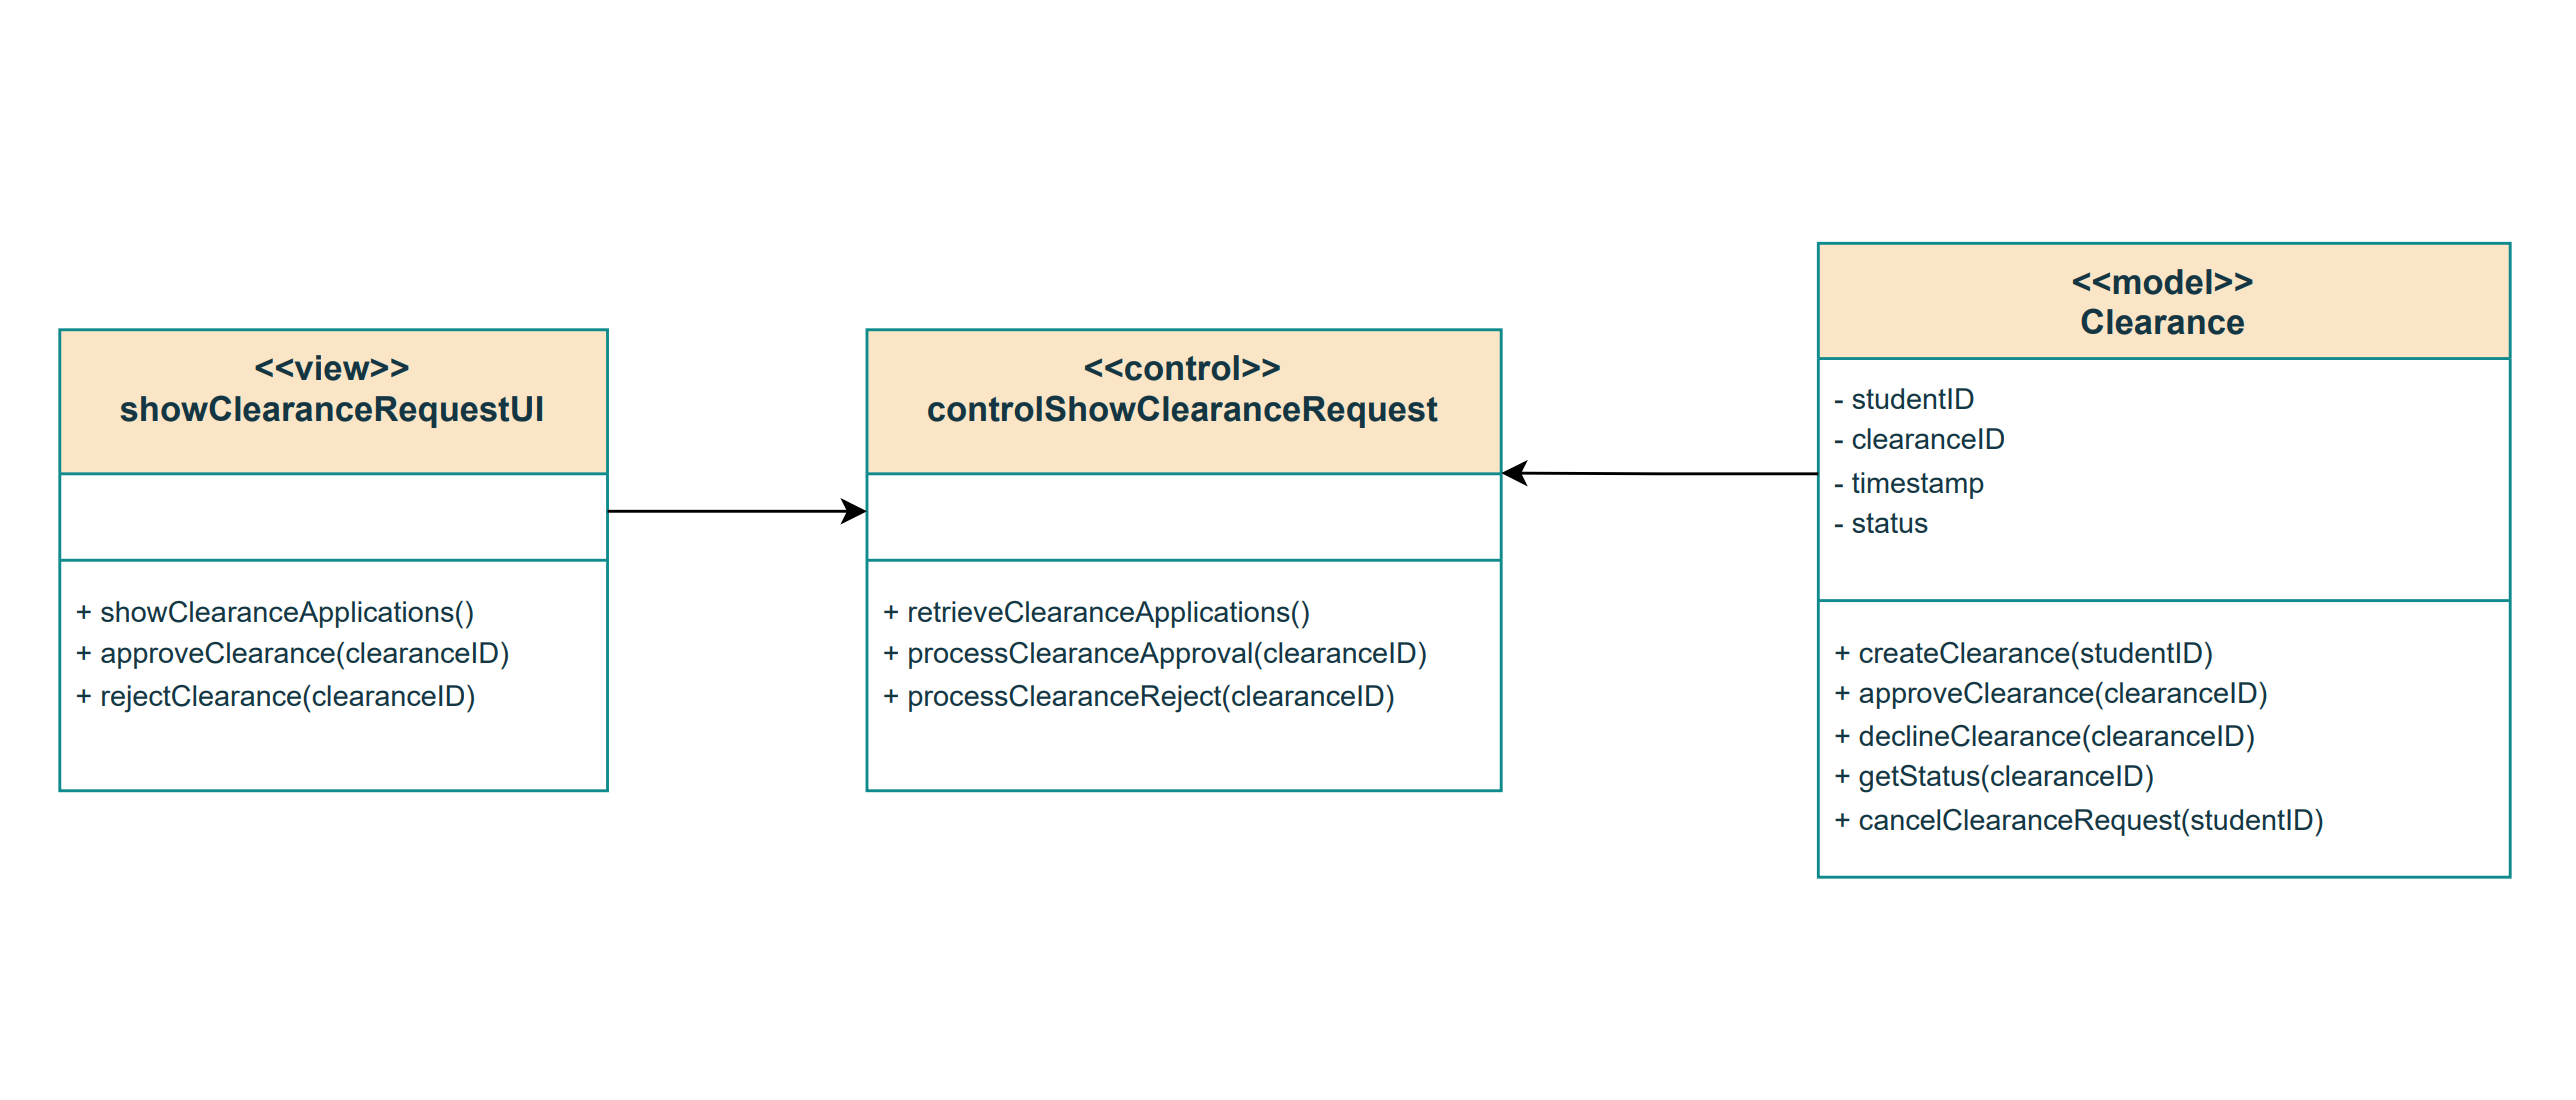
\includegraphics[width= 0.9\textwidth , height= 0.6\paperheight]{ResponseClearanceRequestsUML.png}
        \caption{Response on Clearance Request}
        \label{fig:12}
    \end{figure}

\end{frame}

\begin{frame}{Monetary Dues Class Diagram}

     \begin{figure}
        \centering
        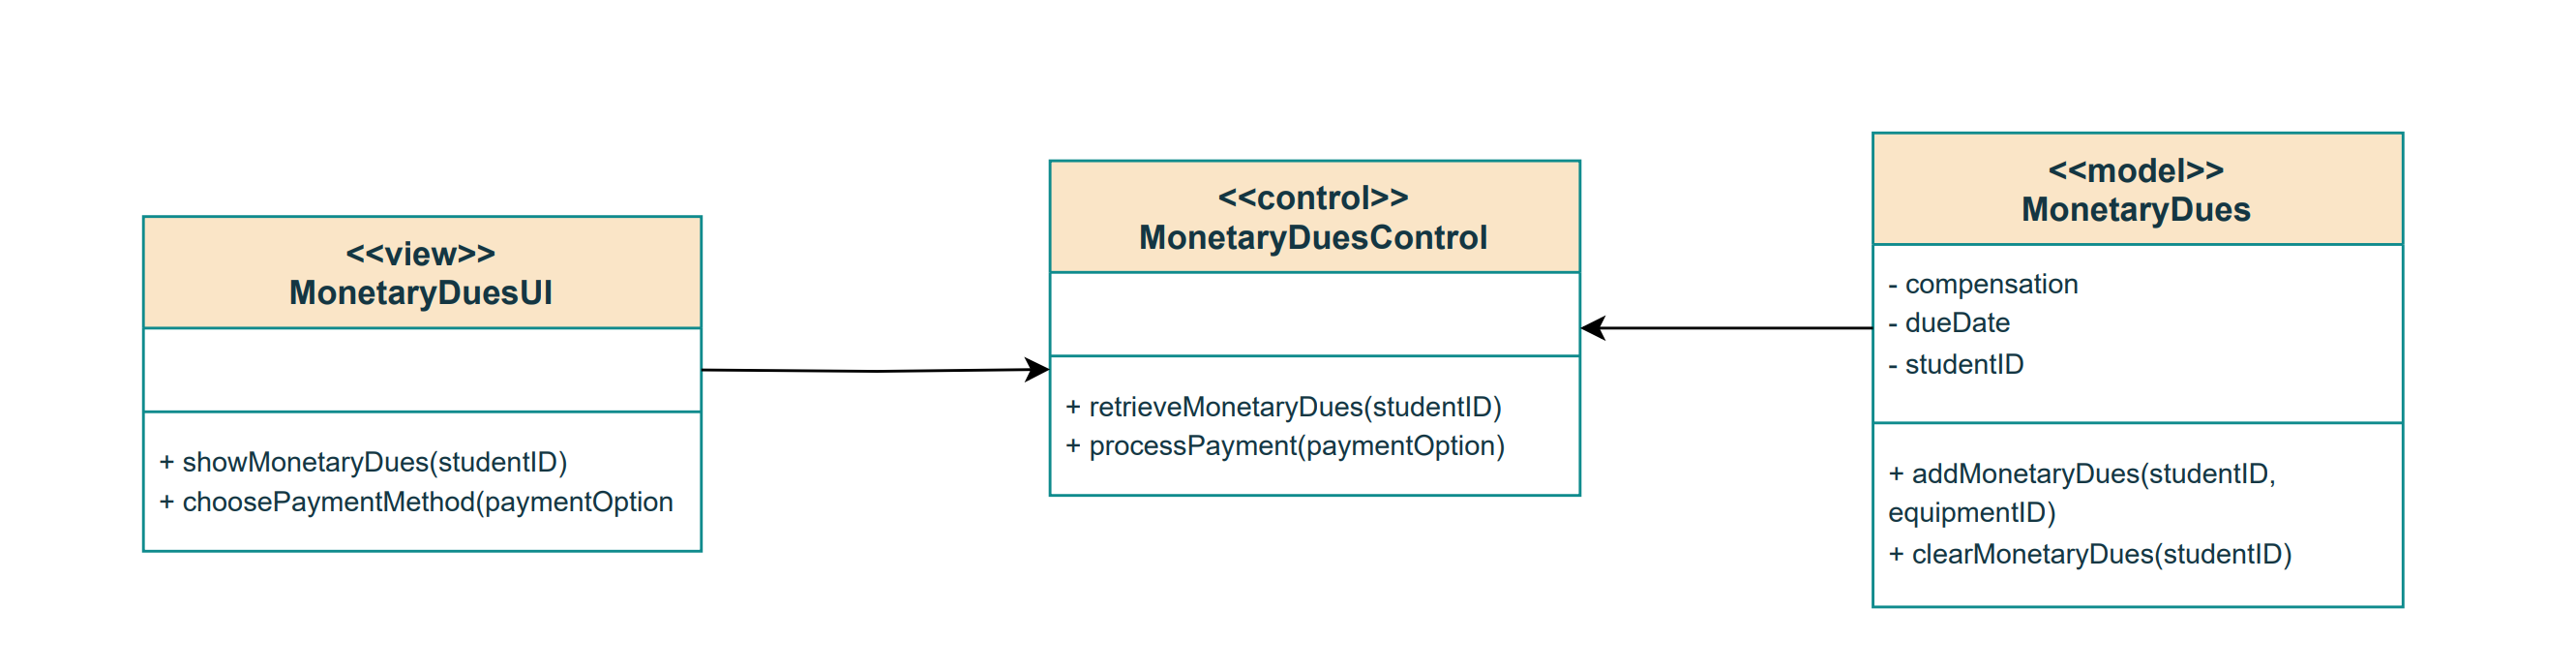
\includegraphics[width= 0.9\textwidth , height= 0.4\paperheight]{MonetaryDuesUML.png}
        \caption{{Pending Monetary Dues}}
        \label{fig:13}
    \end{figure}

\end{frame}

\begin{frame}{Messages Class Diagram}

     \begin{figure}
        \centering
        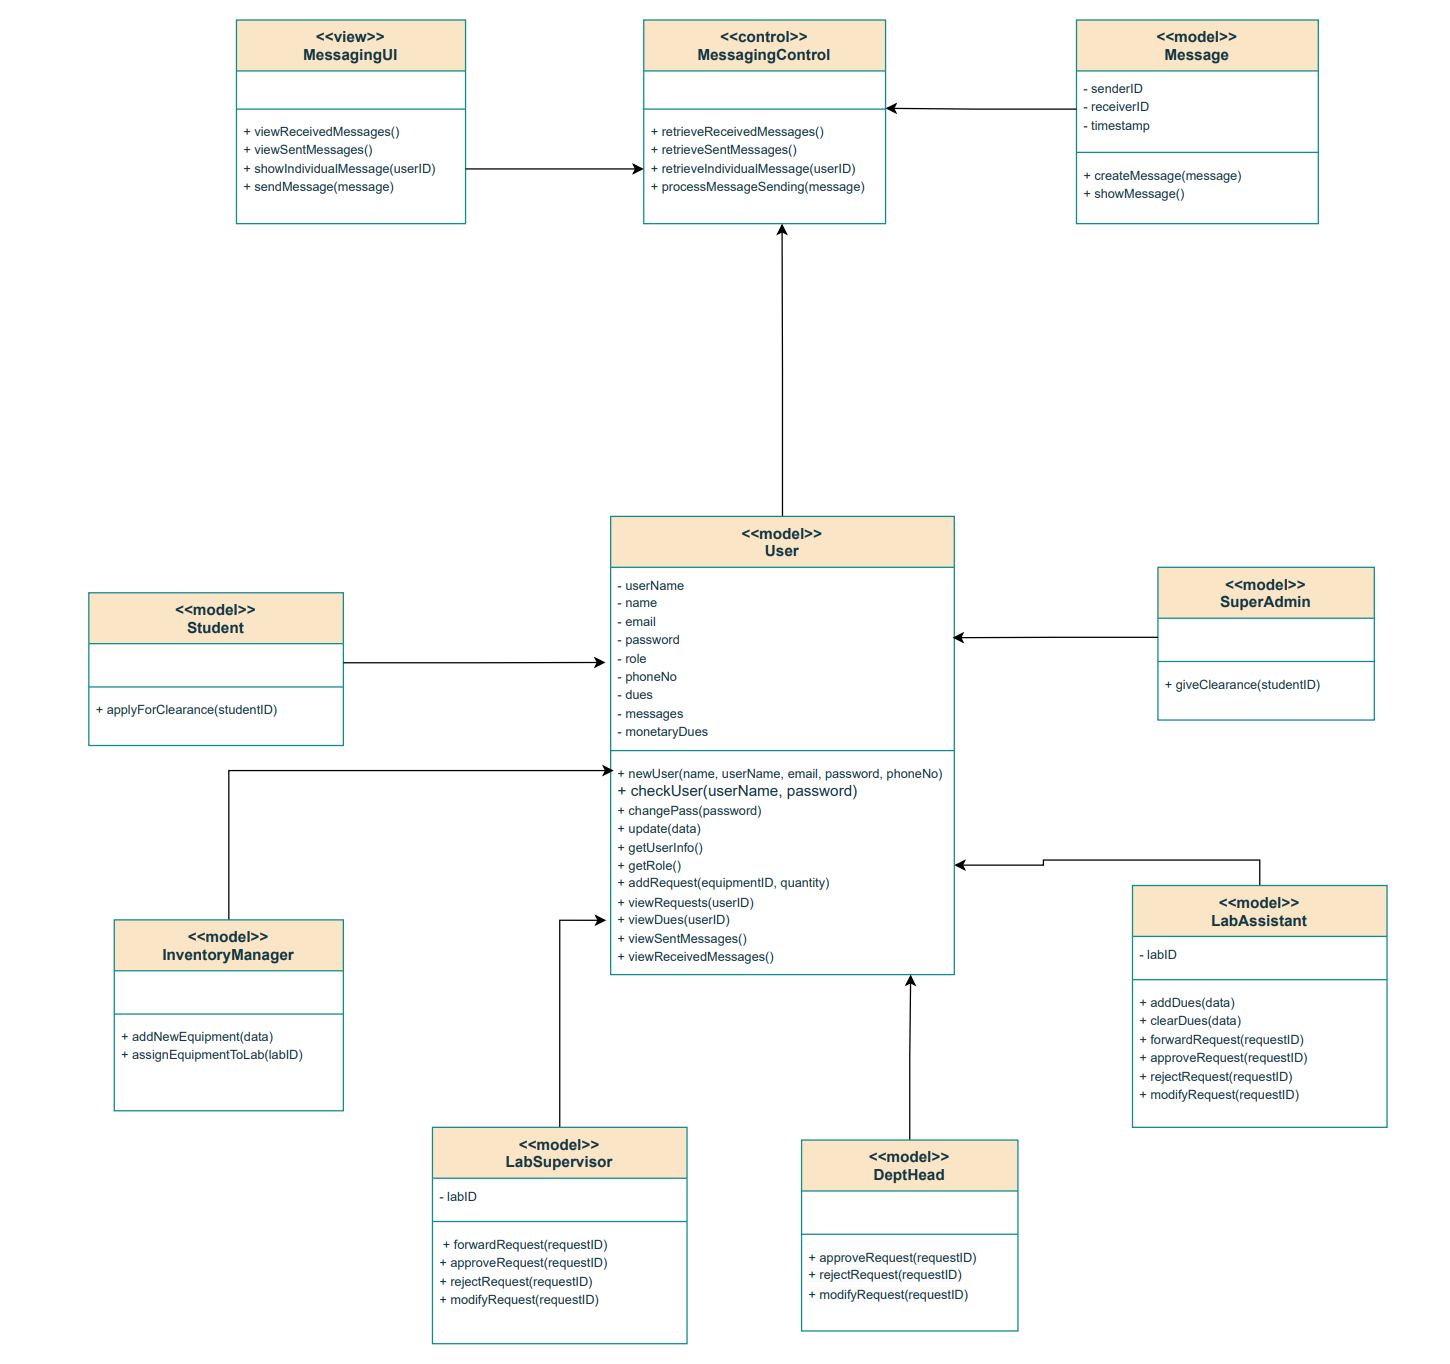
\includegraphics[width= 0.9\textwidth , height= 0.8\paperheight]{MessagesUML.png}
        \caption{Messages}
        \label{fig:14}
    \end{figure}

\end{frame}

\begin{frame}{View Dues Class Diagram}

     \begin{figure}
        \centering
        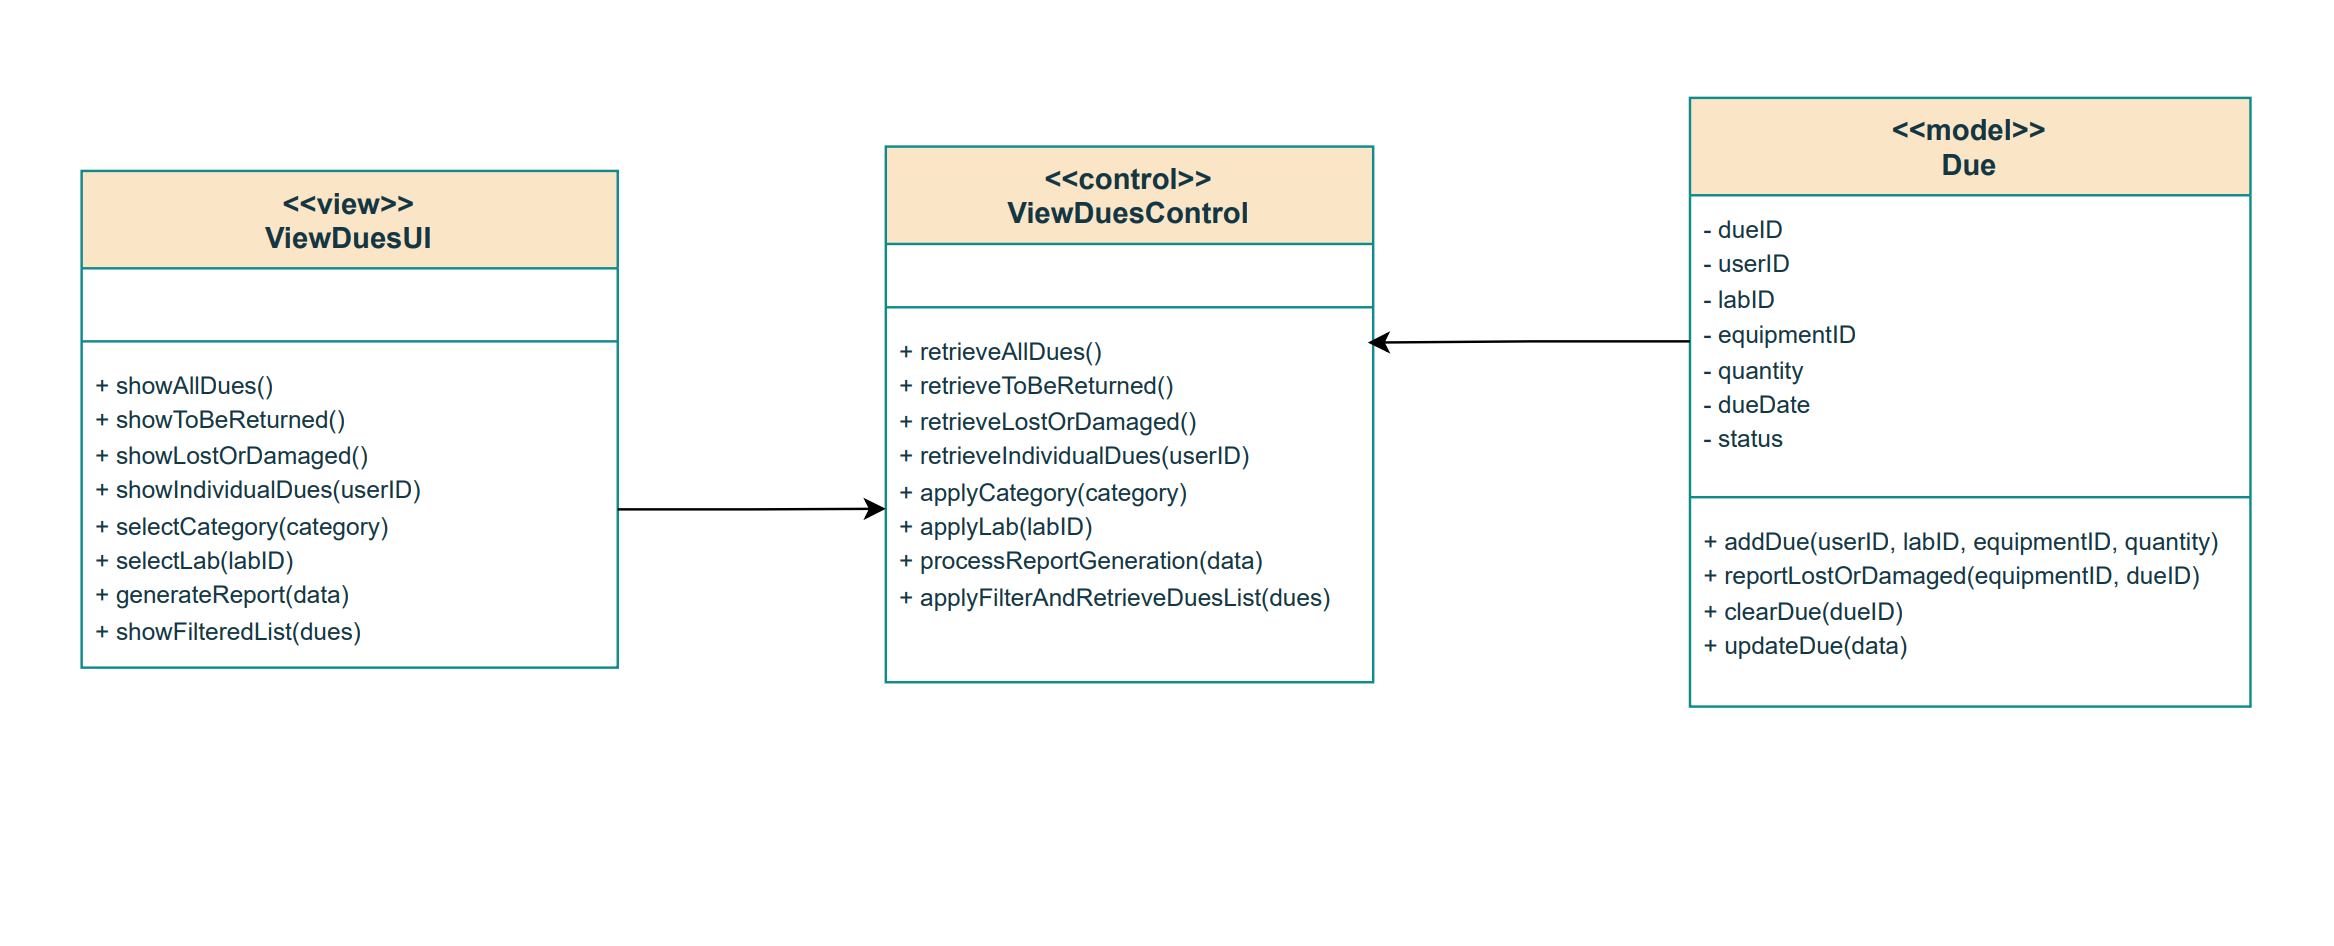
\includegraphics[width= 0.9\textwidth , height= 0.4\paperheight]{ViewDuesUML.png}
        \caption{View Dues}
        \label{fig:15}
    \end{figure}

\end{frame}

\begin{frame}{Check Storage Class Diagram}

     \begin{figure}
        \centering
        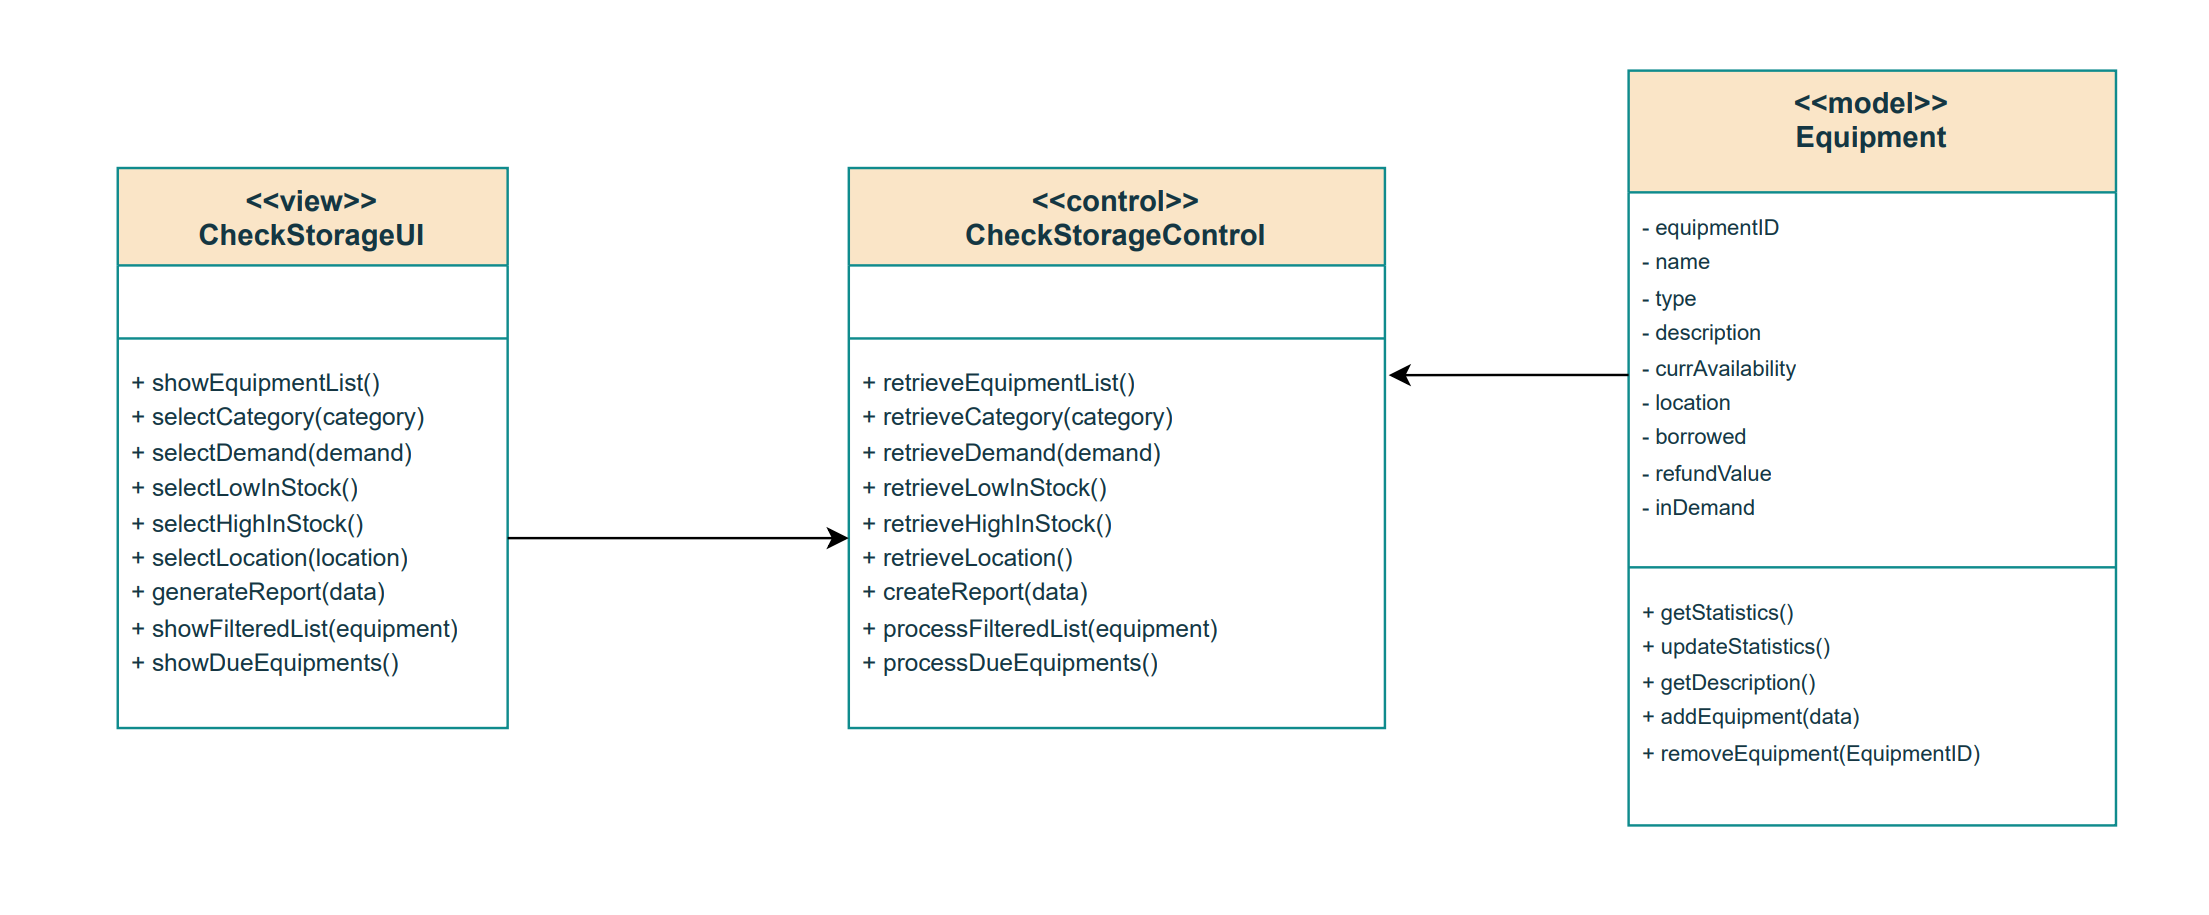
\includegraphics[width= 0.9\textwidth , height= 0.4\paperheight]{CheckStorageUML.png}
        \caption{Check Storage}
        \label{fig:16}
    \end{figure}

\end{frame}

\section{Collaboration Diagram}

\begin{frame}{Home Page Collaboration Diagram}

     \begin{figure}
        \centering
        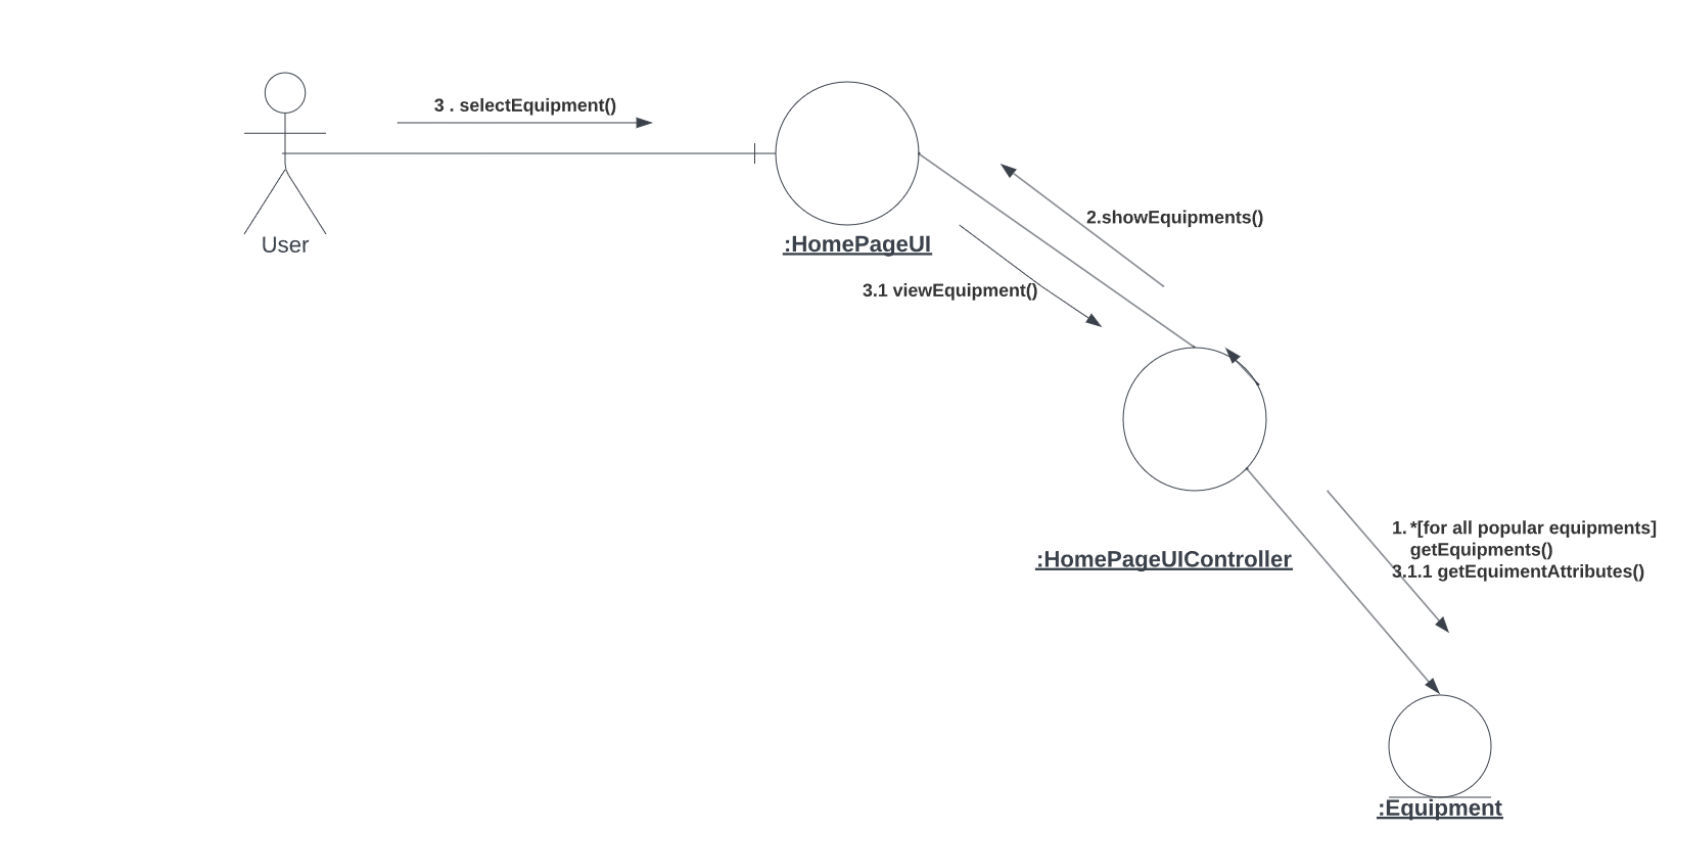
\includegraphics[width= 0.9\textwidth , height= 0.6\paperheight]{HomePageCollab.png}
        \caption{Home Page}
        \label{fig:18}
    \end{figure}

\end{frame}

\begin{frame}{View Equipments Collaboration Diagram}

     \begin{figure}
        \centering
        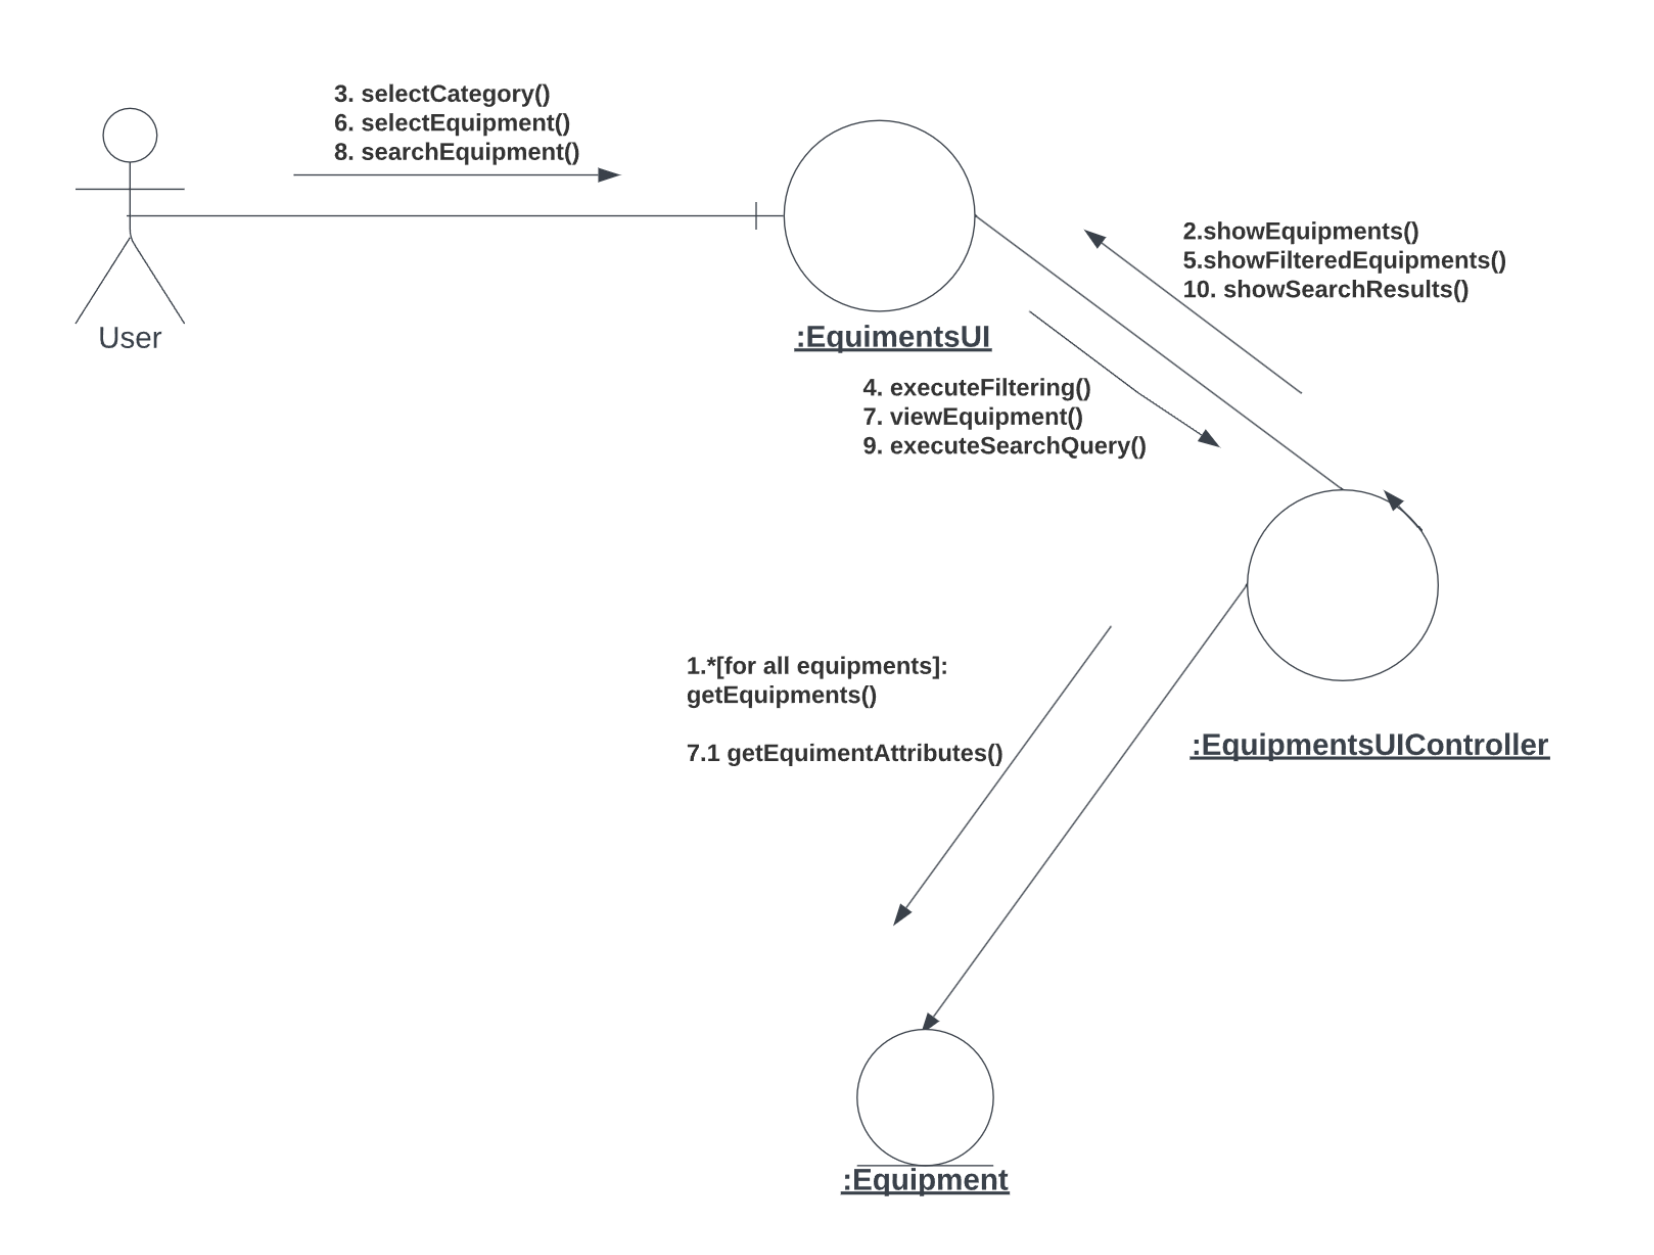
\includegraphics[width= 0.9\textwidth , height= 0.6\paperheight]{EquipmentsViewCollab.png}
        \caption{View Equipments}
        \label{fig:19}
    \end{figure}

\end{frame}

\begin{frame}{Individual Equipments Collaboration Diagram}

     \begin{figure}
        \centering
        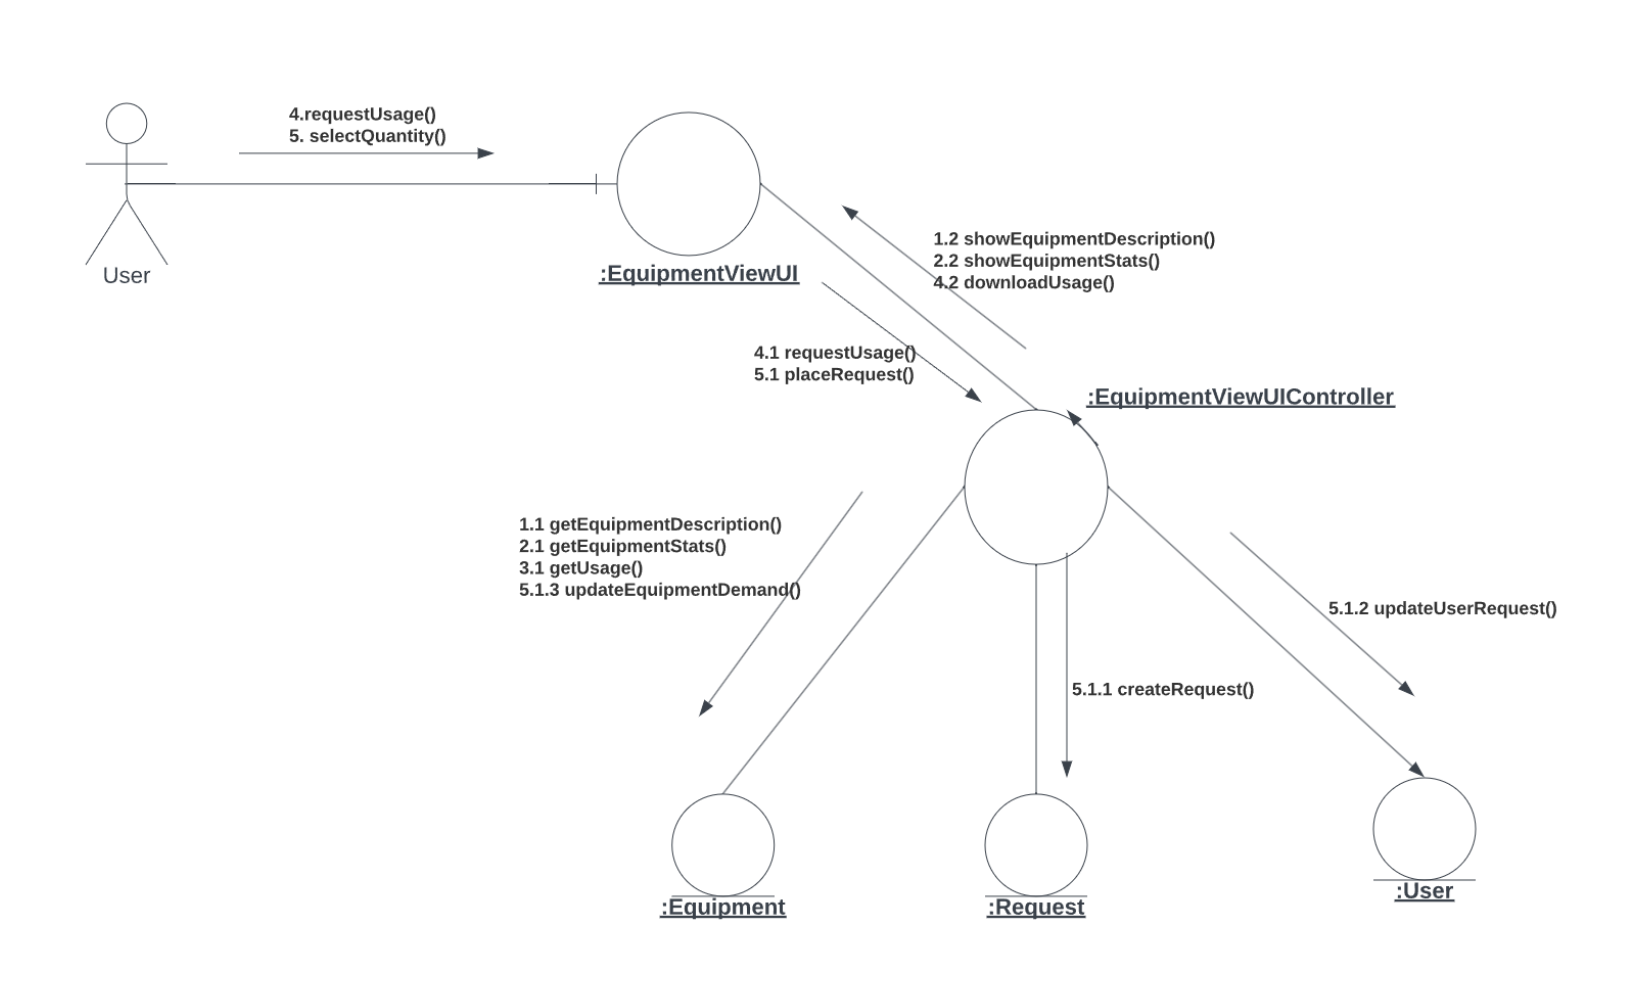
\includegraphics[width= 0.9\textwidth , height= 0.6\paperheight]{IndividualEquipmentCollab.png}
        \caption{Individual Equipments}
        \label{fig:20}
    \end{figure}

\end{frame}

\begin{frame}{Add New Equipments Collaboration Diagram}

     \begin{figure}
        \centering
        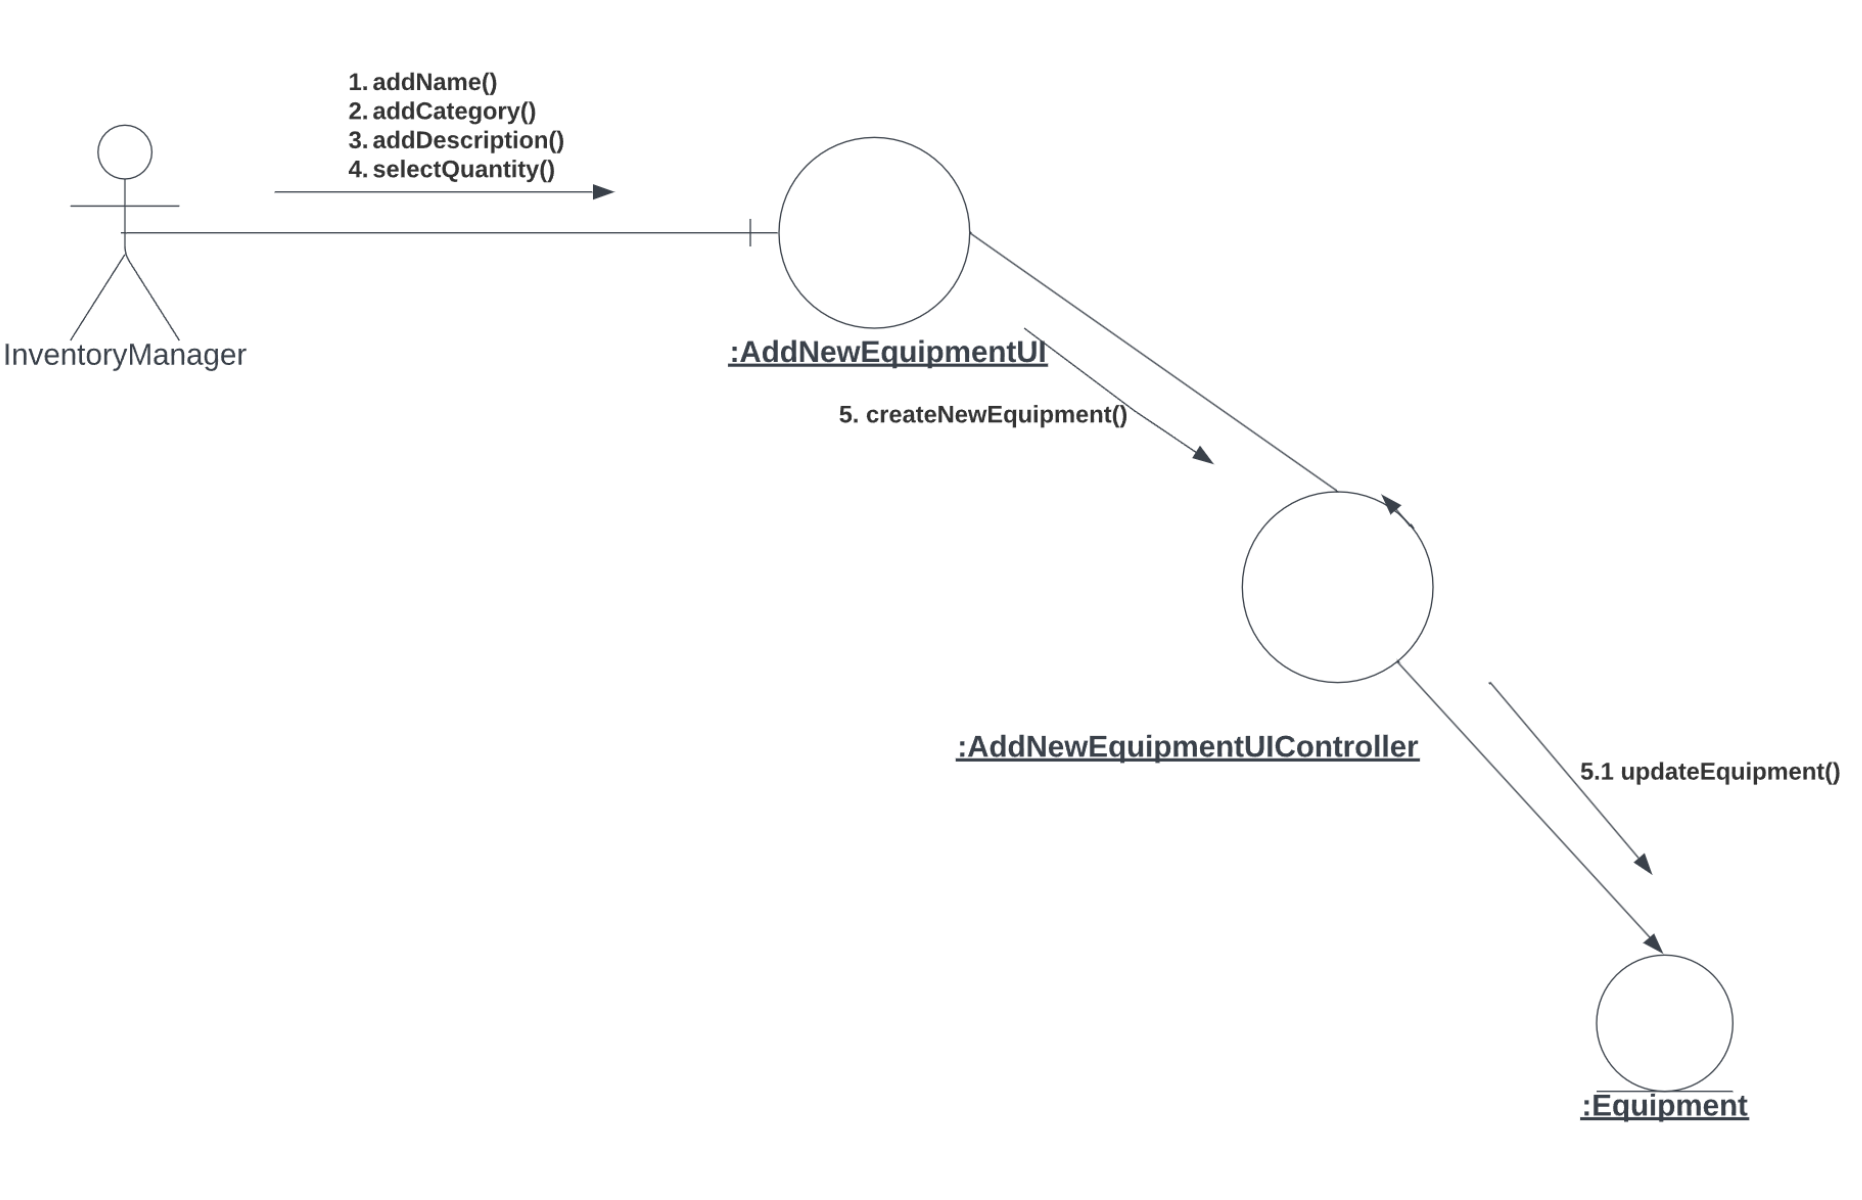
\includegraphics[width= 0.9\textwidth , height= 0.6\paperheight]{AddNewEquipmentCollab.png}
        \caption{Add New Equipments}
        \label{fig:21}
    \end{figure}

\end{frame}

\begin{frame}{Add Equipments Collaboration Diagram}

     \begin{figure}
        \centering
        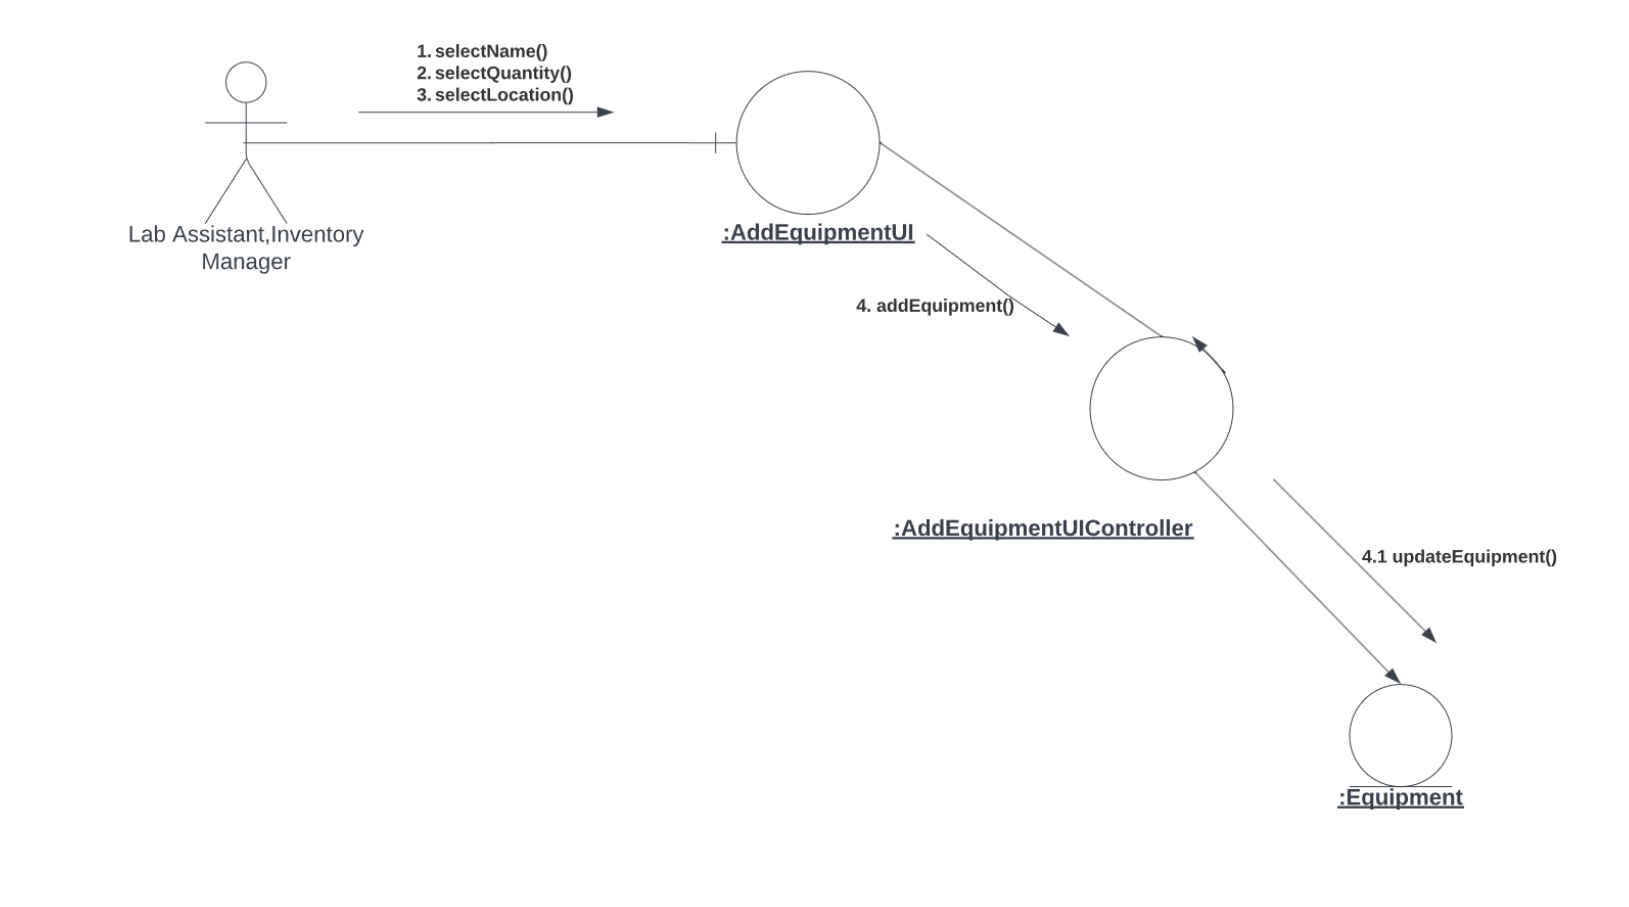
\includegraphics[width= 0.9\textwidth , height= 0.6\paperheight]{AddEquipmentsCollab.png}
        \caption{Add Equipments}
        \label{fig:22}
    \end{figure}

\end{frame}

\begin{frame}{Manage Requests Collaboration Diagram}

     \begin{figure}
        \centering
        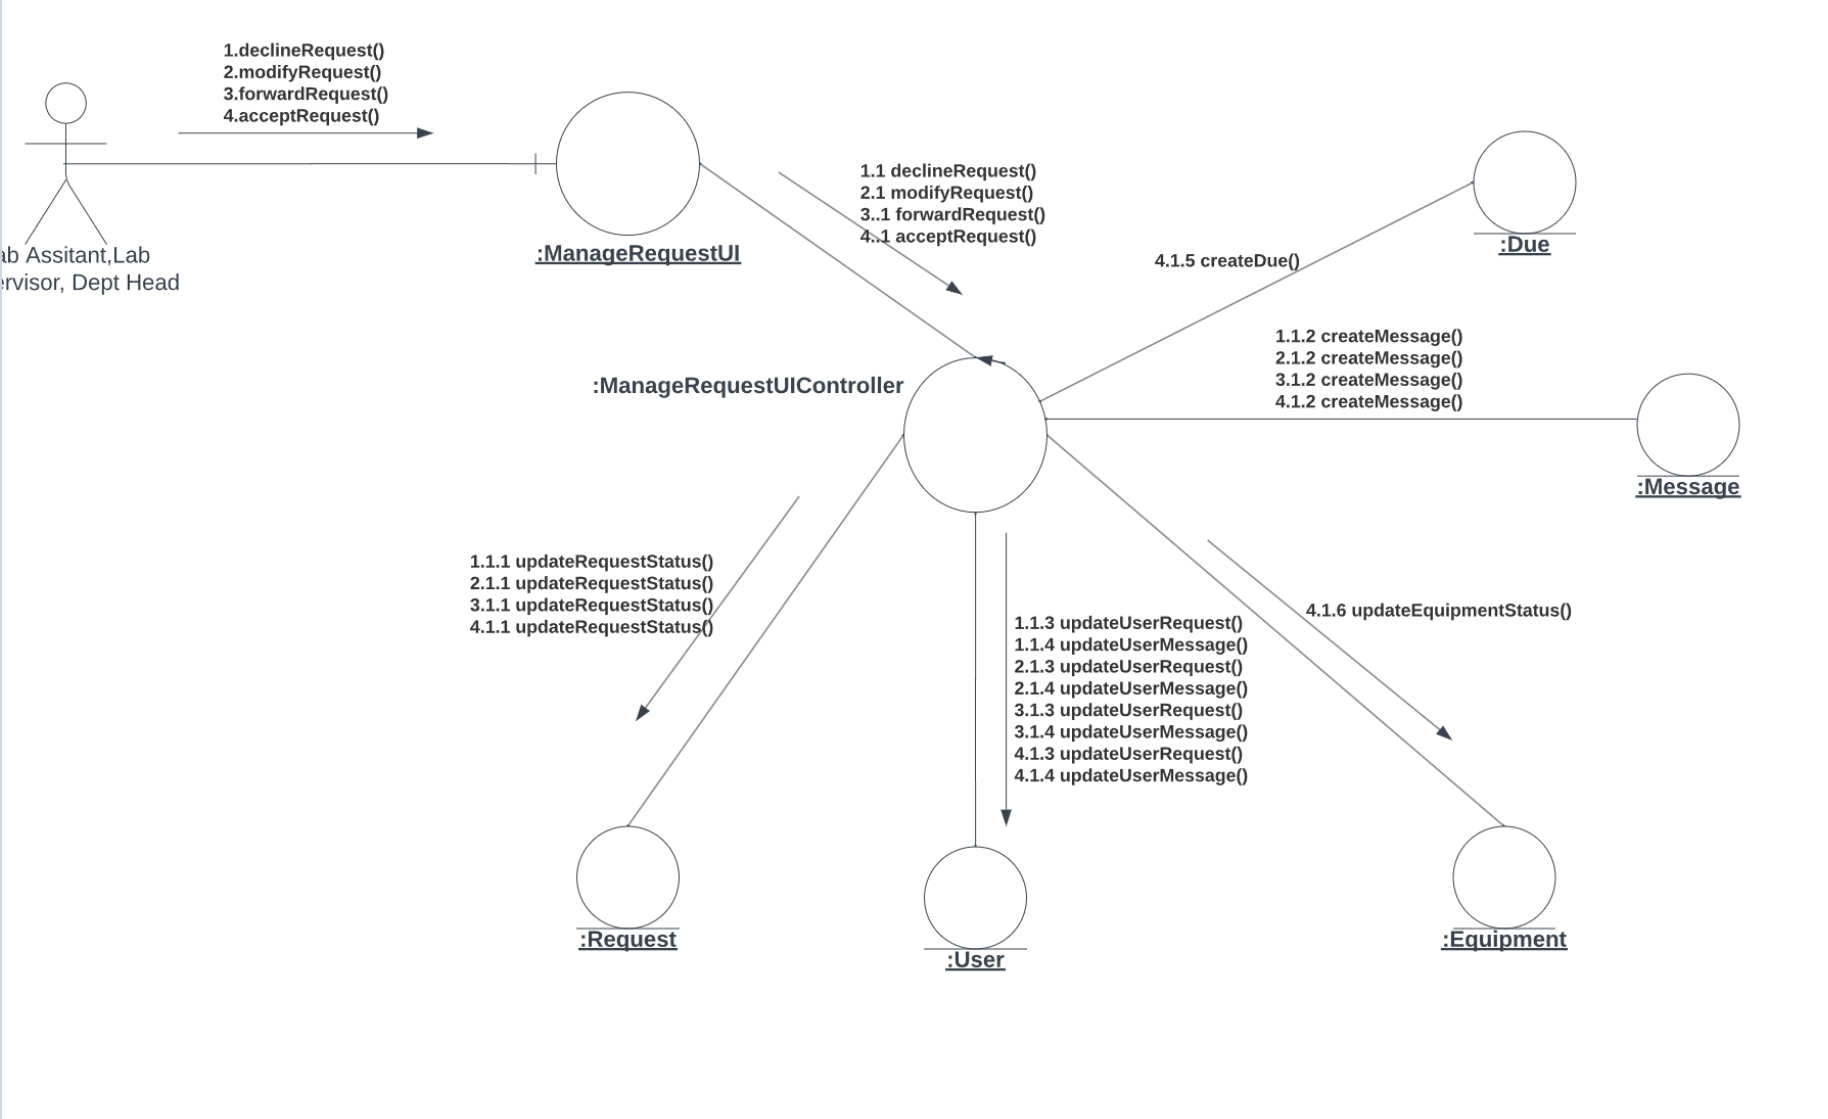
\includegraphics[width= 0.9\textwidth , height= 0.6\paperheight]{ManageRequestCollab.png}
        \caption{Manage Requests}
        \label{fig:23}
    \end{figure}

\end{frame}

\begin{frame}{Messages Collaboration Diagram}

     \begin{figure}
        \centering
        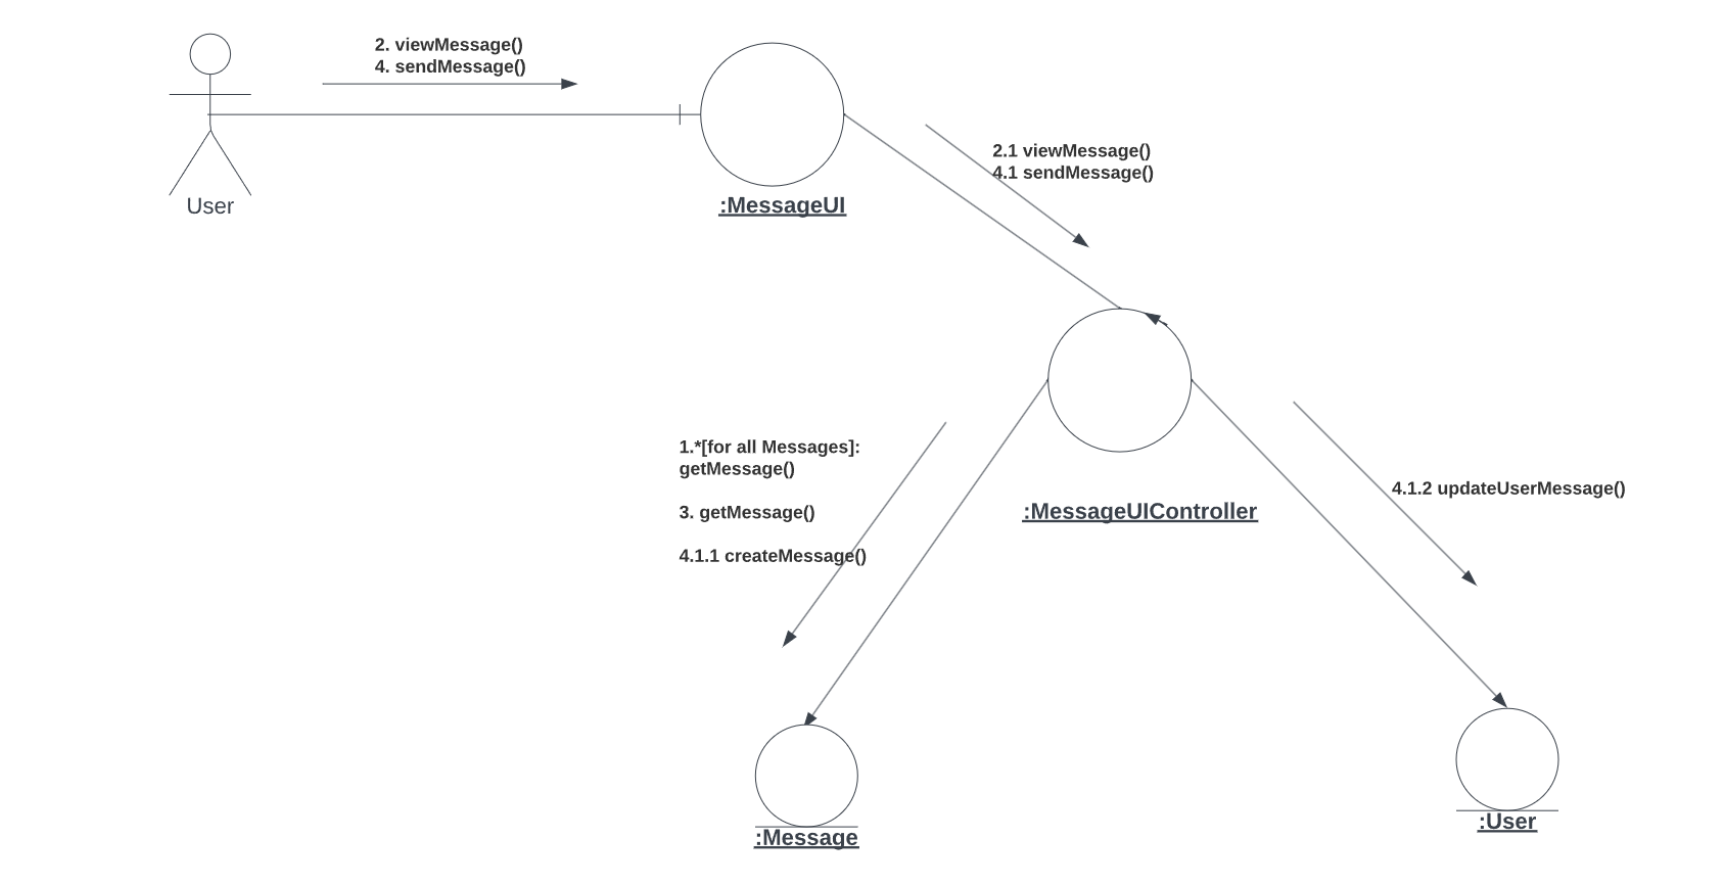
\includegraphics[width= 0.9\textwidth , height= 0.4\paperheight]{MessagesCollab.png}
        \caption{Manage Messages}
        \label{fig:24}
    \end{figure}

\end{frame}

\begin{frame}{View Dues Collaboration Diagram}

     \begin{figure}
        \centering
        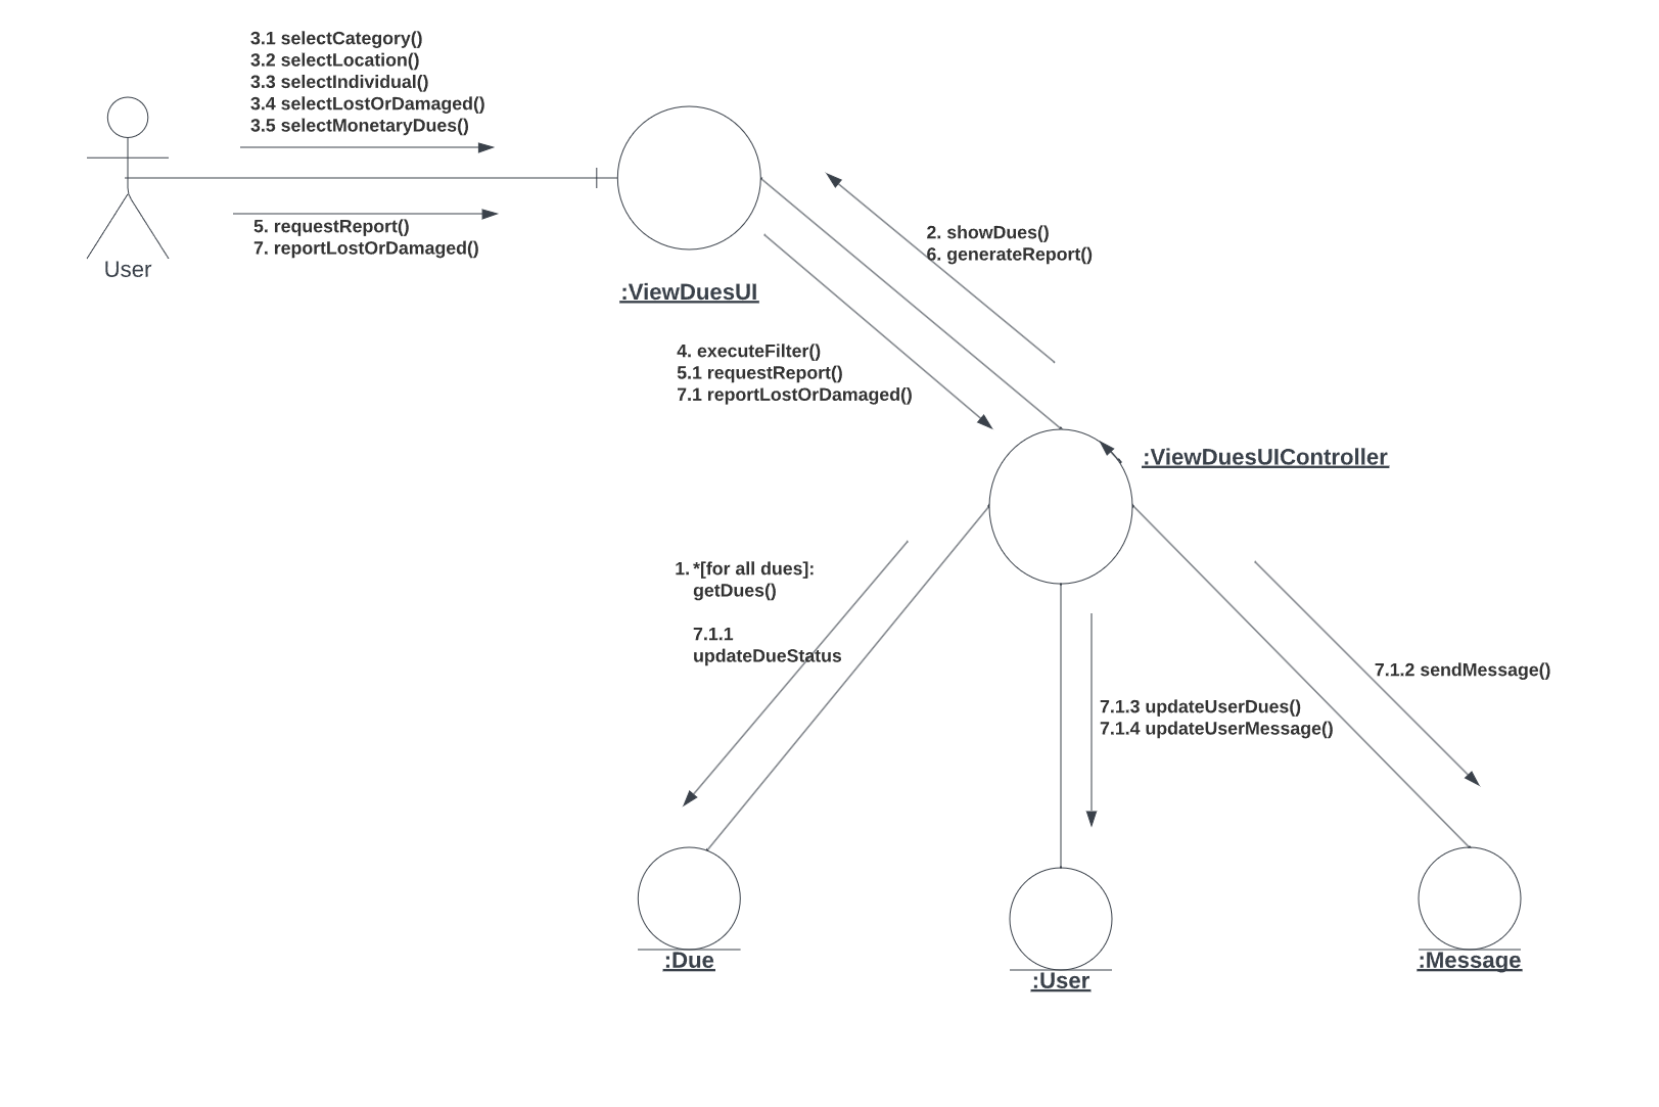
\includegraphics[width= 0.9\textwidth , height= 0.6\paperheight]{ViewDuesCollab.png}
        \caption{View Dues}
        \label{fig:25}
    \end{figure}

\end{frame}

\begin{frame}{Check Storage Collaboration Diagram}

     \begin{figure}
        \centering
        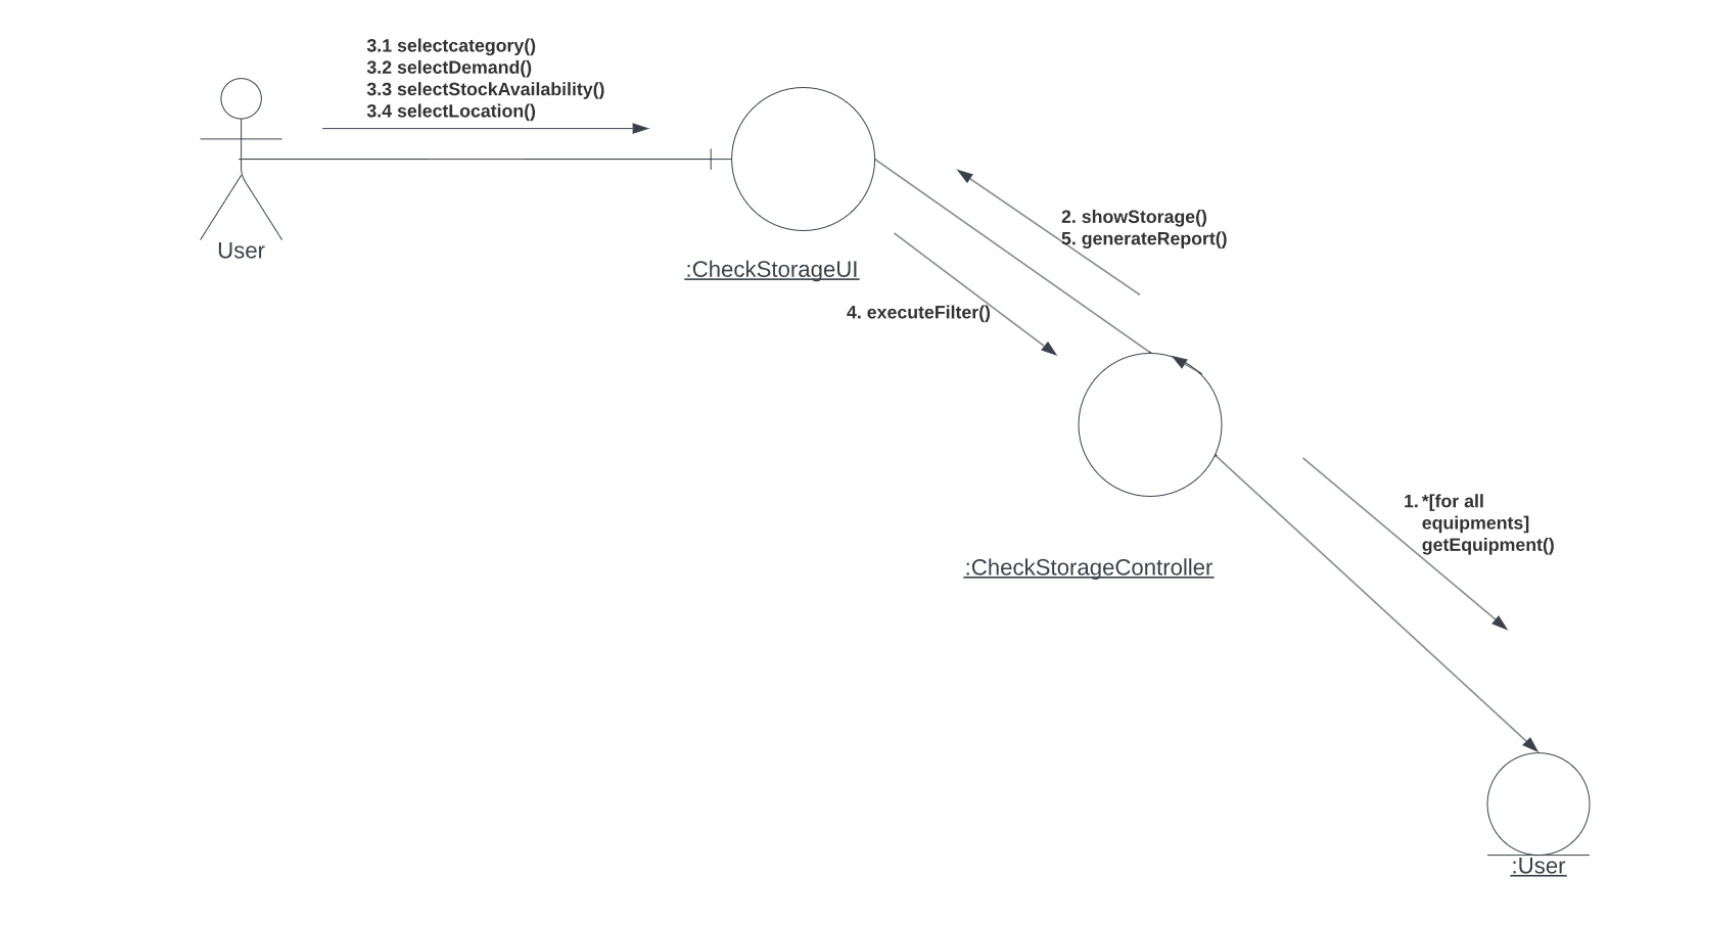
\includegraphics[width= 0.9\textwidth , height= 0.6\paperheight]{CheckStorageCollab.png}
        \caption{Check Storage}
        \label{fig:26}
    \end{figure}

\end{frame}

\begin{frame}{Clearance Grant Collaboration Diagram}

     \begin{figure}
        \centering
        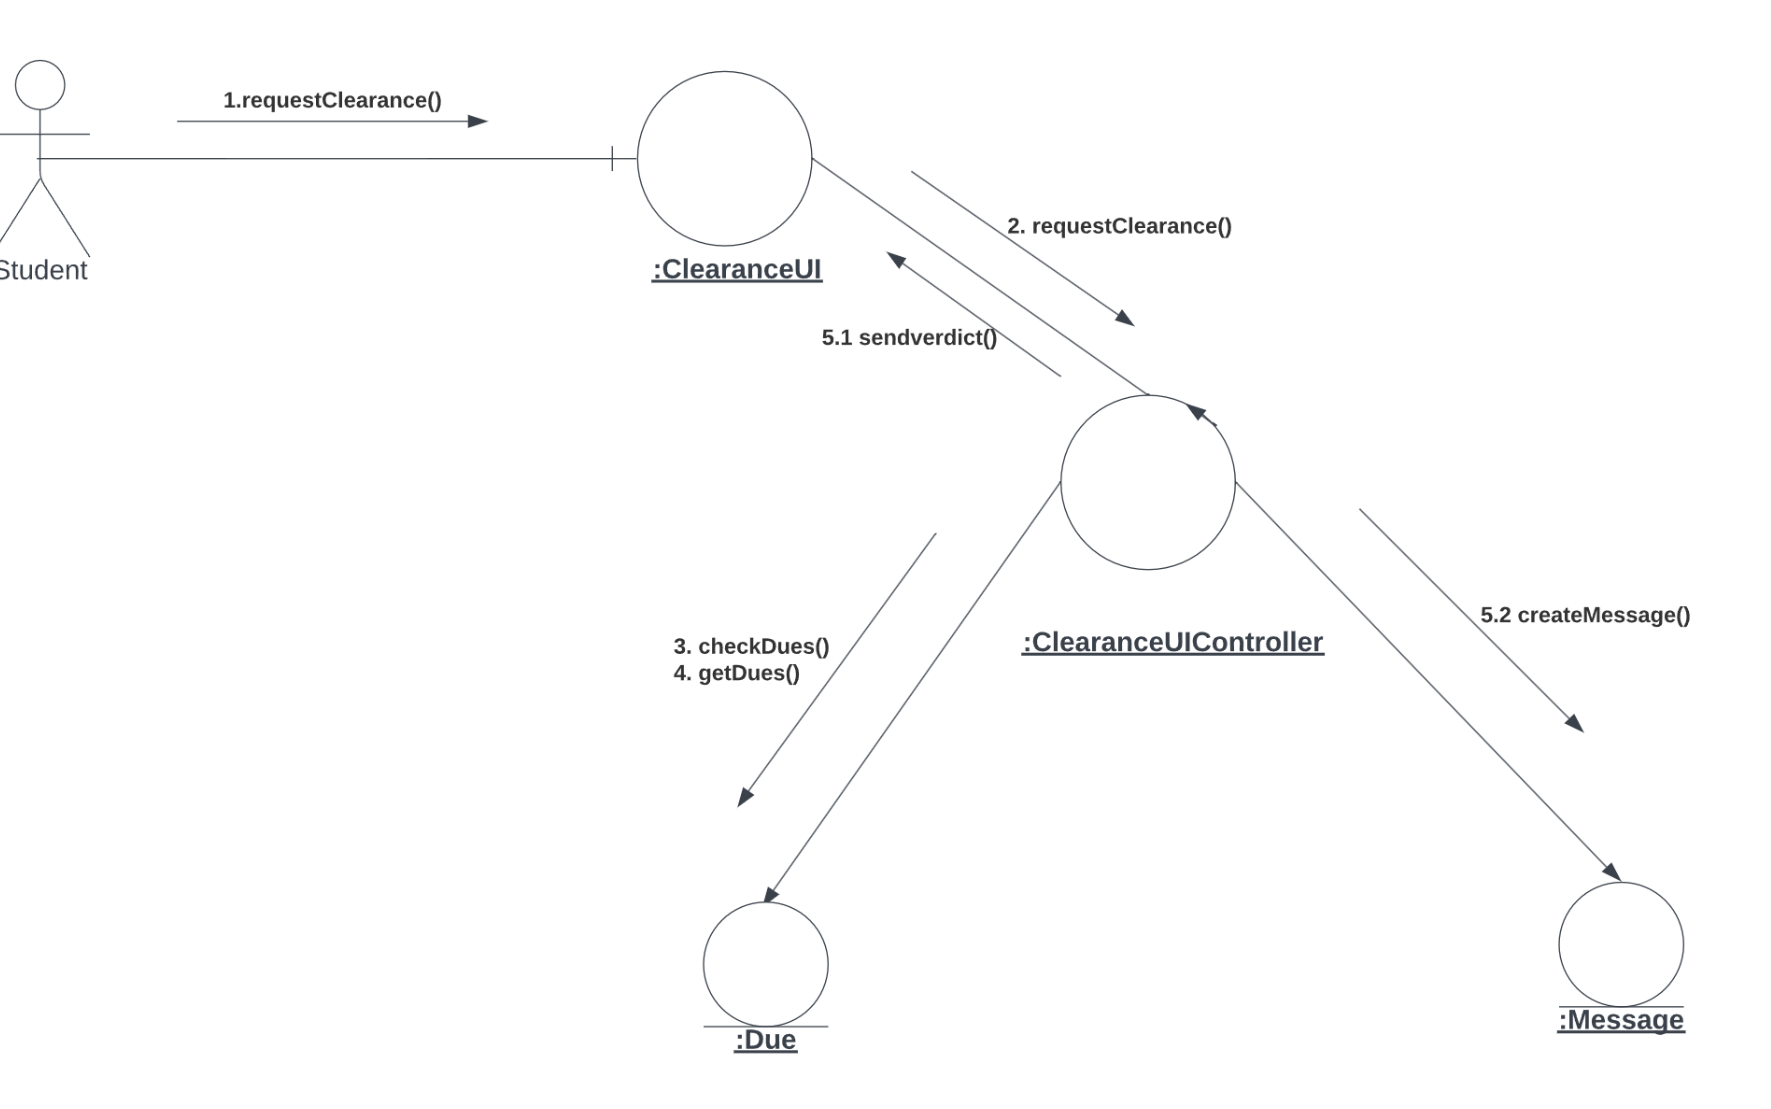
\includegraphics[width= 0.9\textwidth , height= 0.6\paperheight]{ClearanceCollab.png}
        \caption{Clearance Grant}
        \label{fig:27}
    \end{figure}

\end{frame}

\section{Sequence Diagram}

\begin{frame}{Home Page Sequence Diagram}

     \begin{figure}
        \centering
        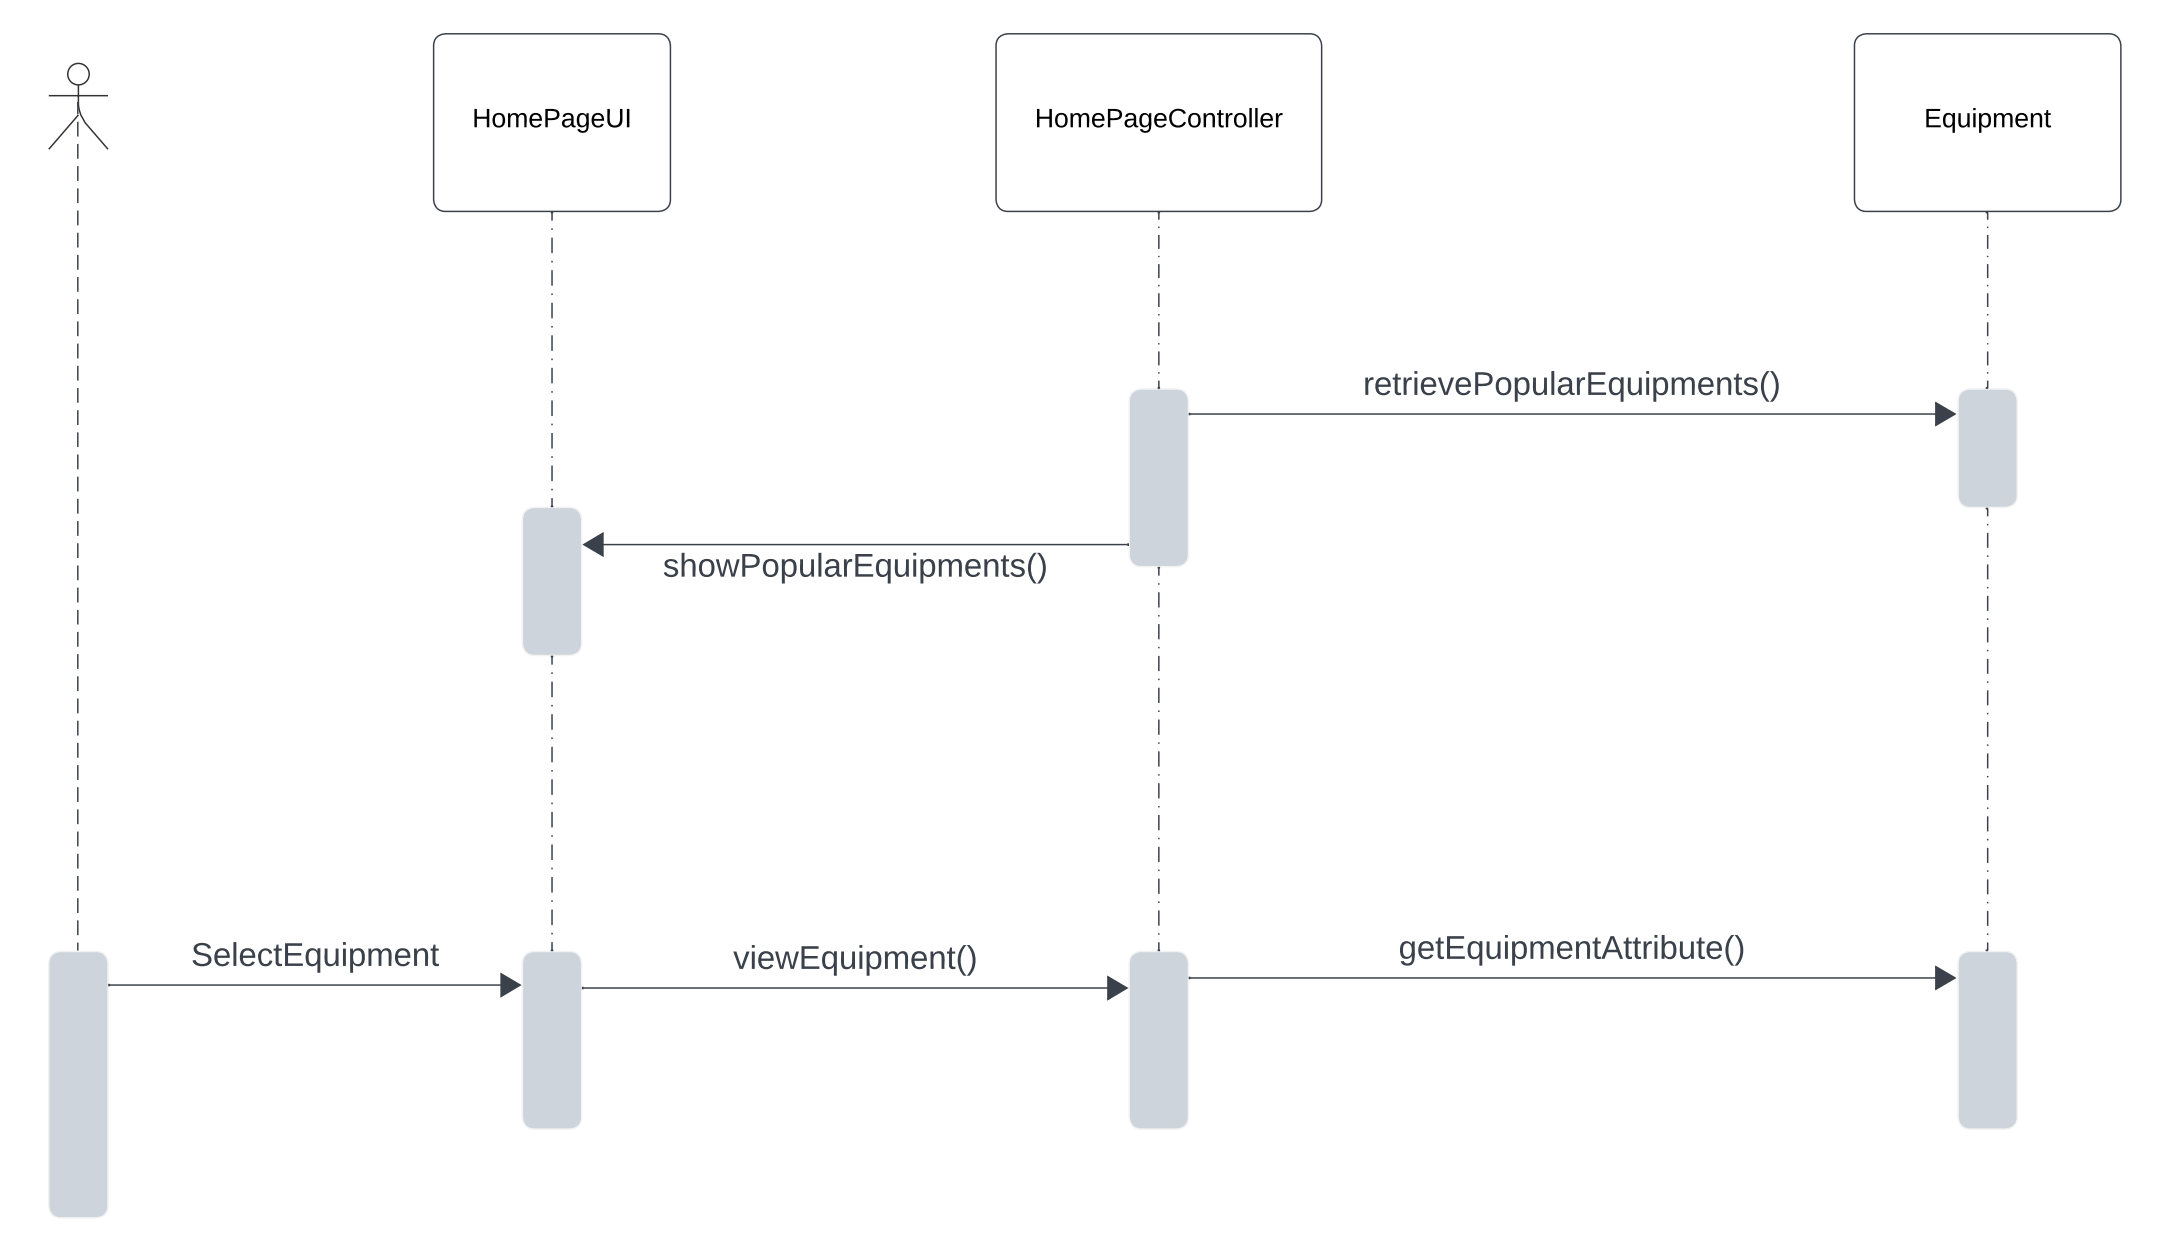
\includegraphics[width= 0.9\textwidth , height= 0.6\paperheight]{HomePageSeq.png}
        \caption{Home Page}
        \label{fig:28}
    \end{figure}

\end{frame}

\begin{frame}{View Equipment Sequence Diagram}

     \begin{figure}
        \centering
        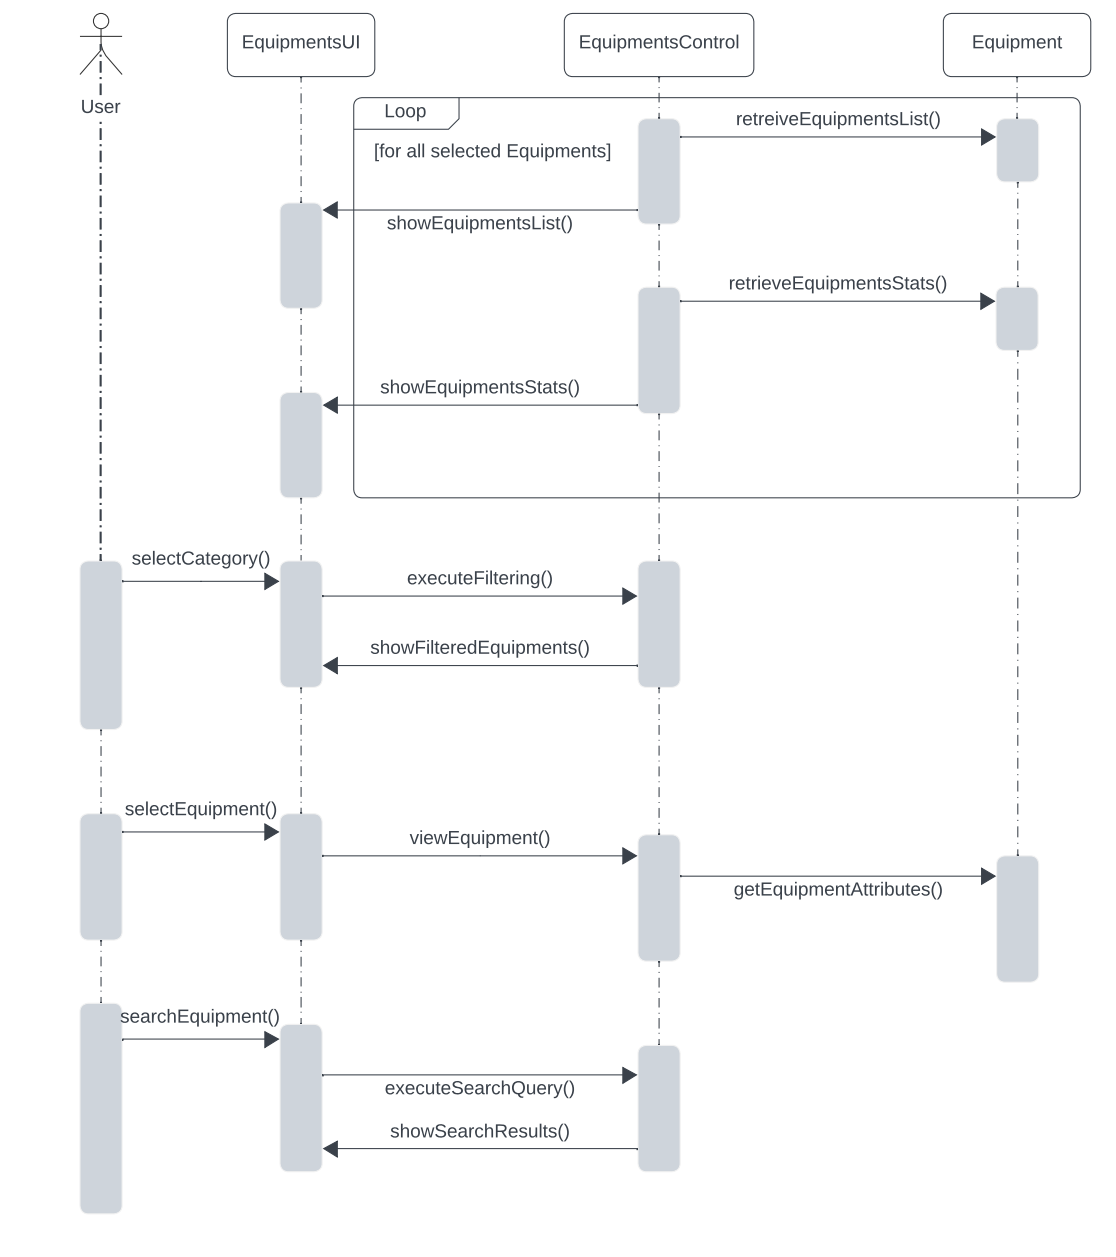
\includegraphics[width= 0.8\textwidth , height= 0.8\paperheight]{EquipmentsViewSeq.png}
        \caption{View Equipments}
        \label{fig:29}
    \end{figure}

\end{frame}

\begin{frame}{Add Equipments Sequence Diagram}

     \begin{figure}
        \centering
        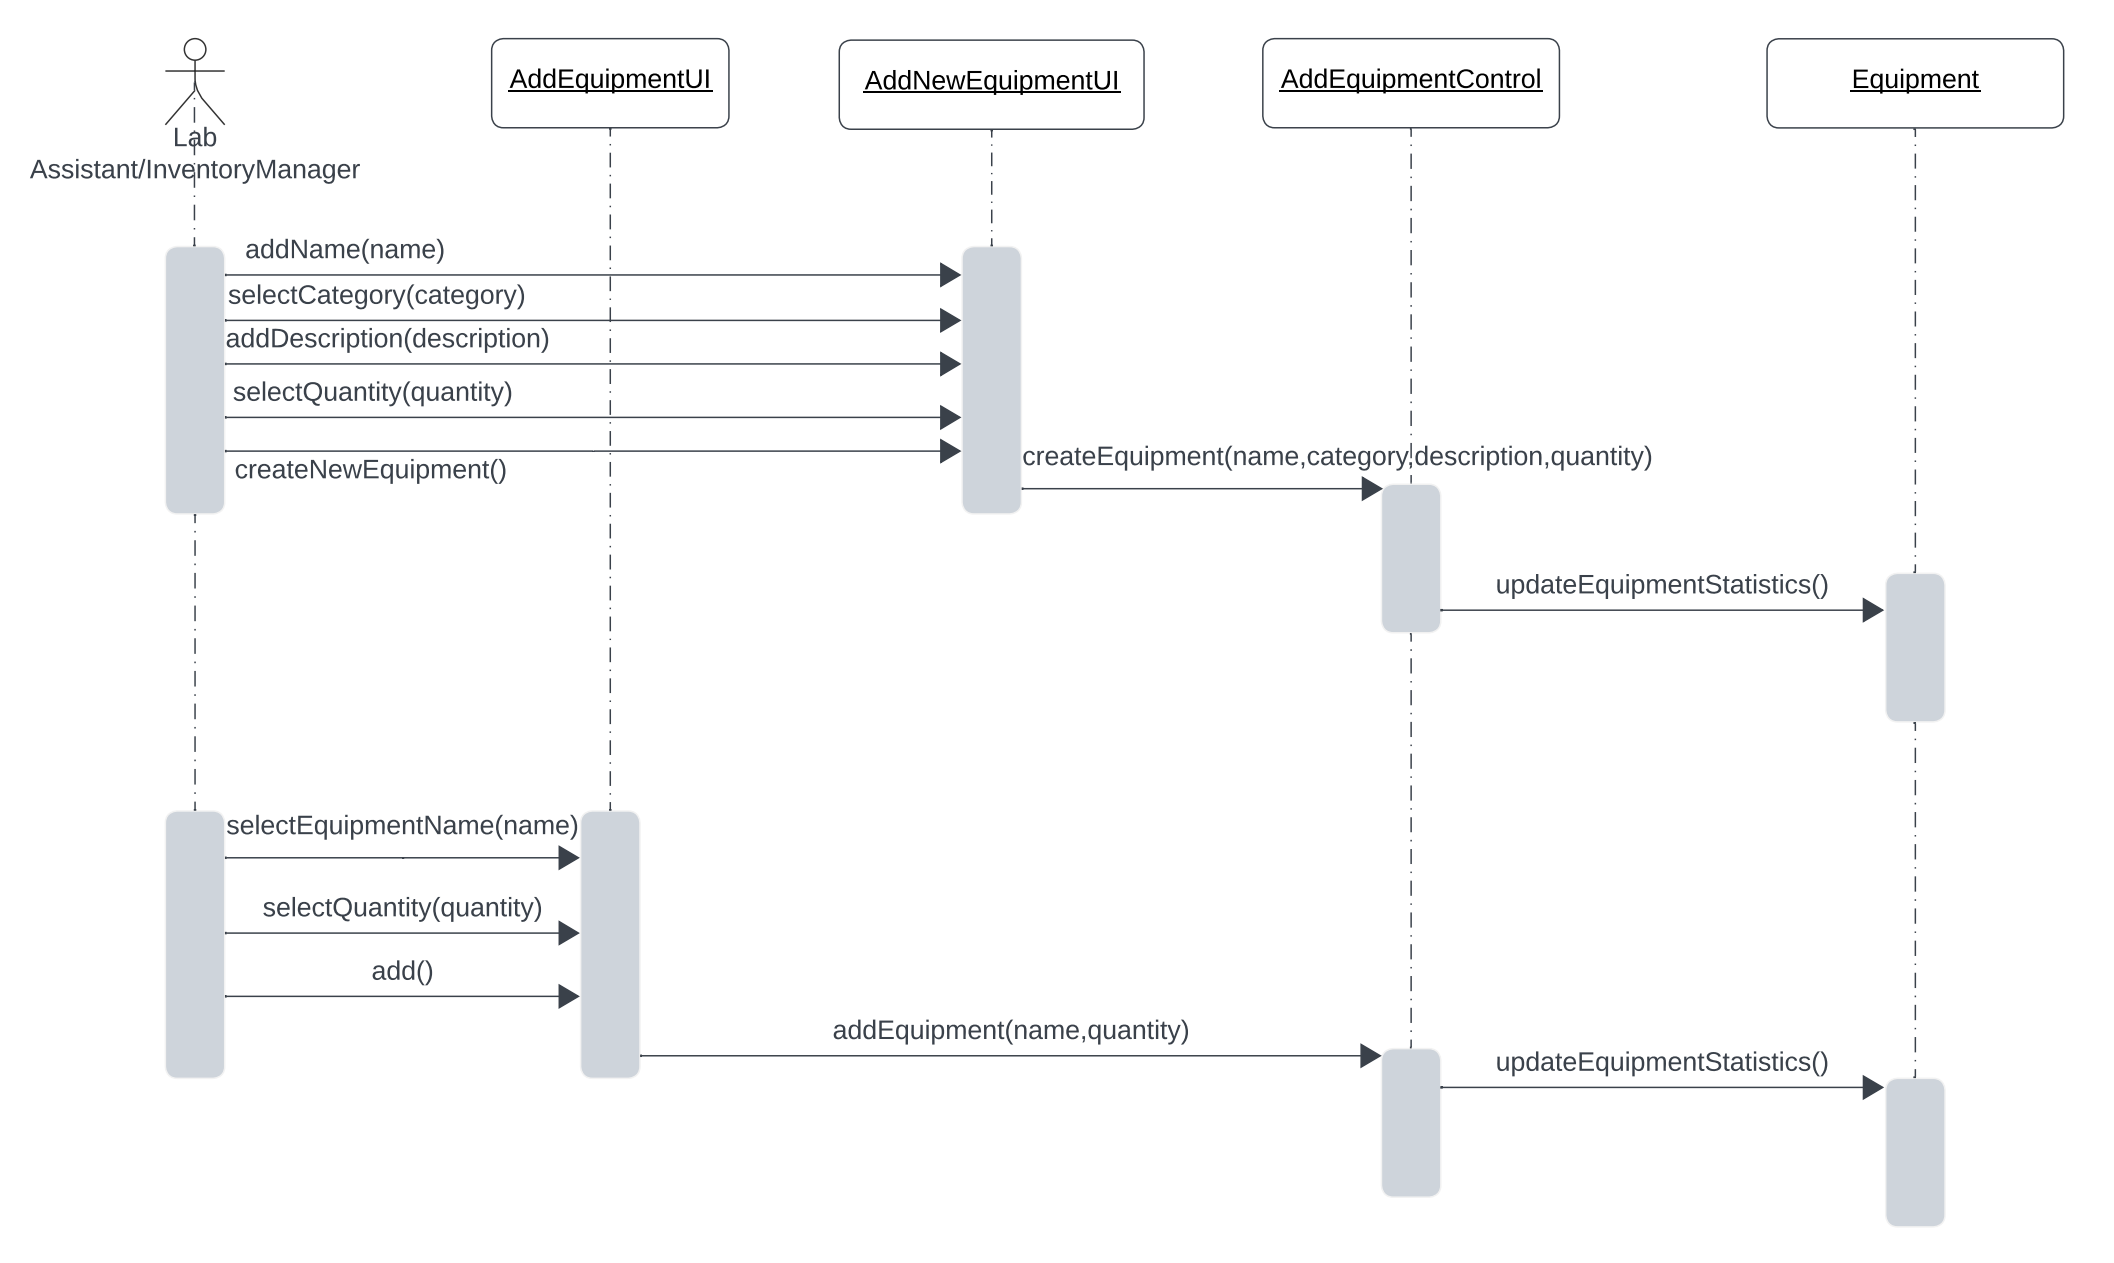
\includegraphics[width= 0.7\textwidth , height= 0.6\paperheight]{AddEquipmentsSeq.png}
        \caption{Add Equipments}
        \label{fig:30}
    \end{figure}

\end{frame}

\begin{frame}{Individual Equipments Sequence Diagram}

     \begin{figure}
        \centering
        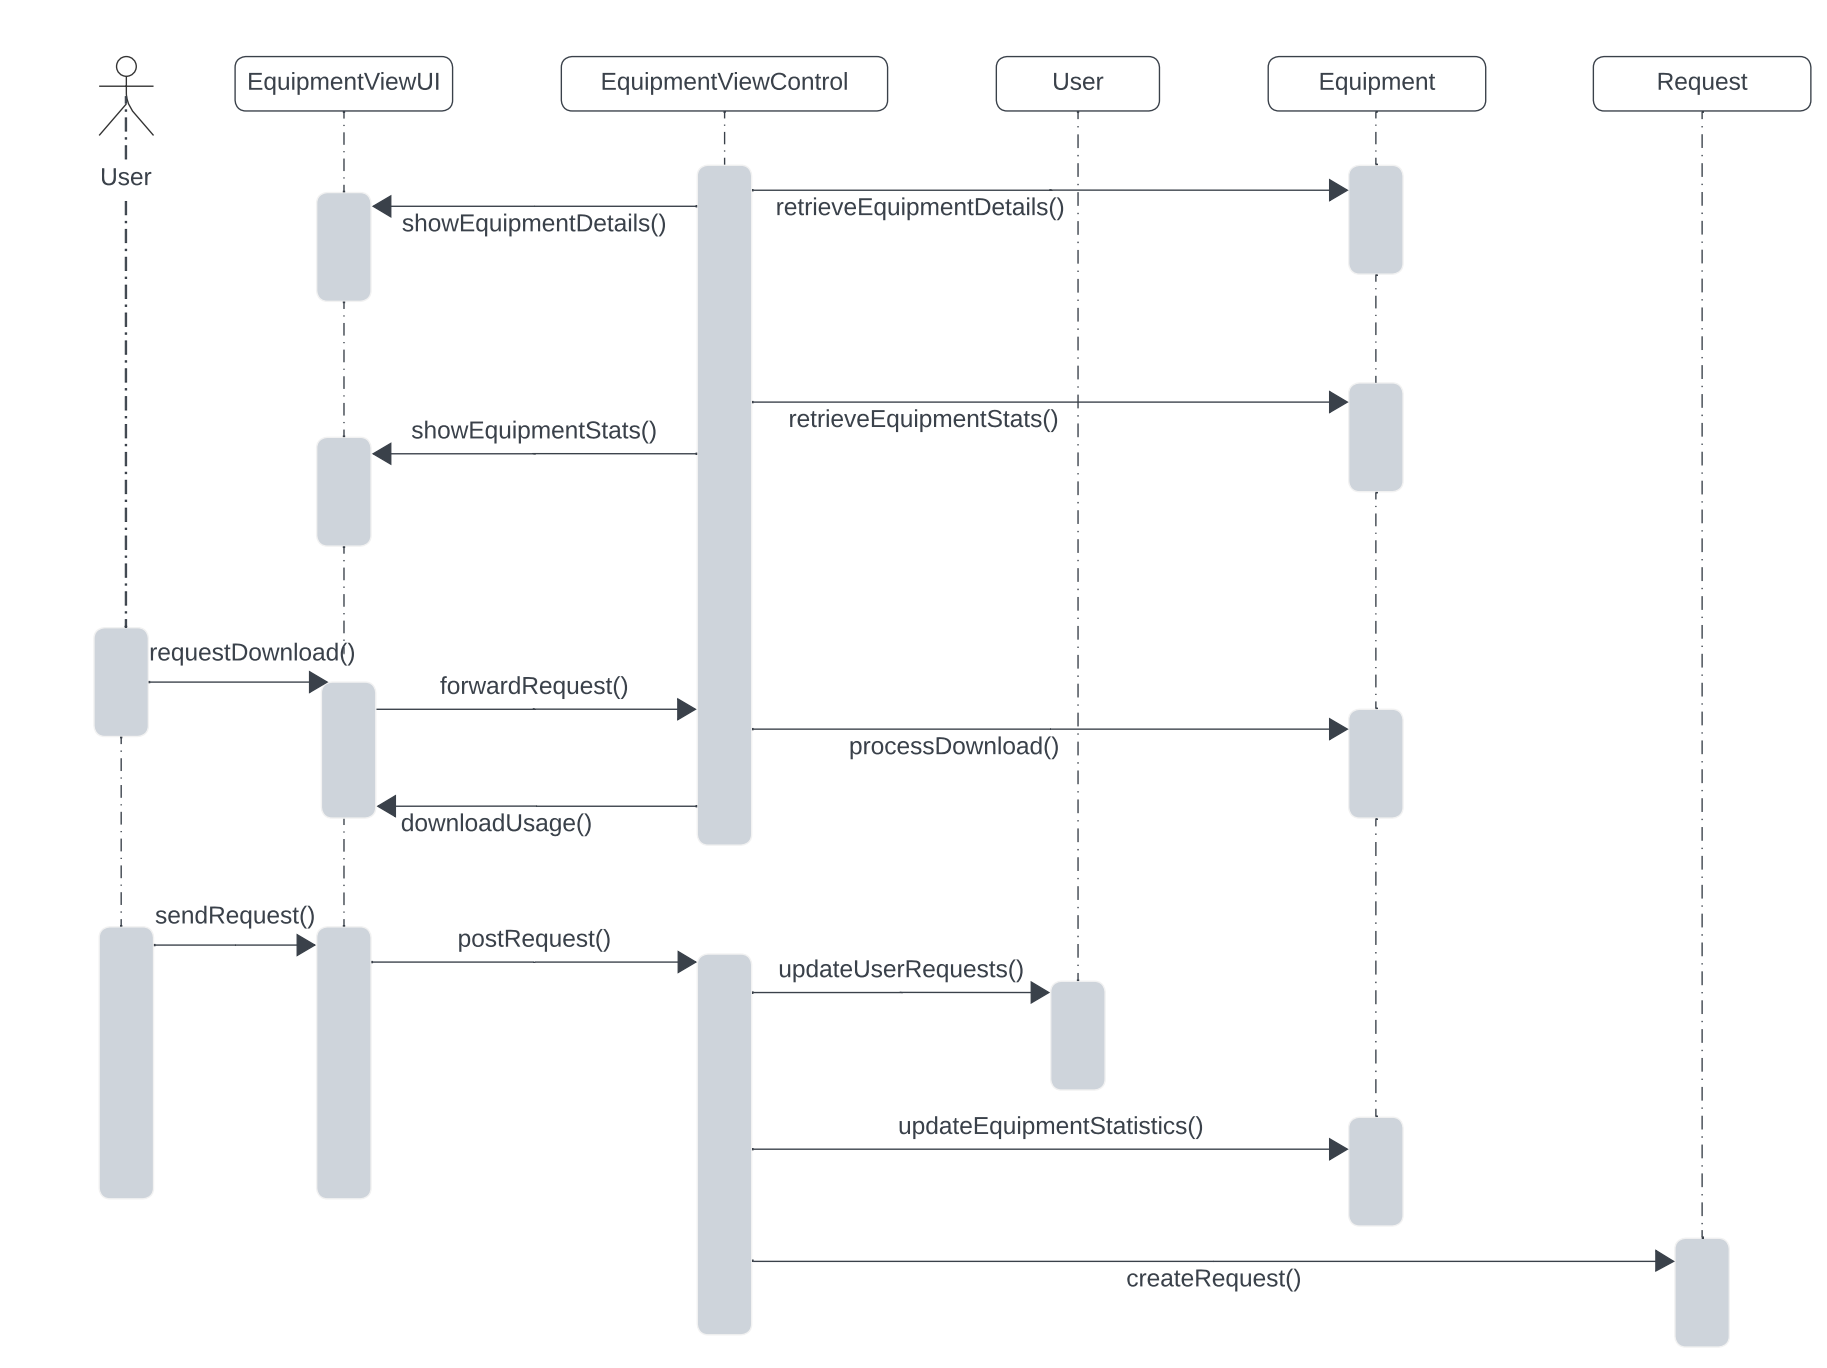
\includegraphics[width= 0.9\textwidth , height= 0.6\paperheight]{IndividualEquipmentseq.png}
        \caption{Individual Equipments}
        \label{fig:31}
    \end{figure}

\end{frame}

\begin{frame}{View Requests Sequence Diagram}

     \begin{figure}
        \centering
        \includegraphics[width= 0.7\textwidth , height= 0.8\paperheight]{ViewRequestsSeq.png}
        \caption{View Requests}
        \label{fig:32}
    \end{figure}

\end{frame}

\begin{frame}{Manage Requests Sequence Diagram}

     \begin{figure}
        \centering
        \includegraphics[width= 0.9\textwidth , height= 0.6\paperheight]{ManageRequestSeq.png}
        \caption{Manage Requests}
        \label{fig:33}
    \end{figure}

\end{frame}

\begin{frame}{View Dues Sequence Diagram}

     \begin{figure}
        \centering
        \includegraphics[width= 0.9\textwidth , height= 0.6\paperheight]{ViewDuesSeq.png}
        \caption{View Dues}
        \label{fig:34}
    \end{figure}

\end{frame}

\begin{frame}{Manage Dues Sequence Diagram}

     \begin{figure}
        \centering
        \includegraphics[width= 0.8\textwidth , height= 0.8\paperheight]{ManageDuesSeq.png}
        \caption{Manage Dues}
        \label{fig:35}
    \end{figure}

\end{frame}

\begin{frame}{Check Storage Sequence Diagram}

     \begin{figure}
        \centering
        \includegraphics[width= 0.8\textwidth , height= 0.6\paperheight]{CheckStorageSeq.png}
        \caption{Check Storage}
        \label{fig:36}
    \end{figure}

\end{frame}

\begin{frame}{Manage Clearance Sequence Diagram}

     \begin{figure}
        \centering
        \includegraphics[width= 0.9\textwidth , height= 0.3\paperheight]{ManageClearanceSeq.png}
        \caption{Manage Clearance}
        \label{fig:37}
    \end{figure}

\end{frame}

\begin{frame}{Messages Sequence Diagram}

     \begin{figure}
        \centering
        \includegraphics[width= 0.9\textwidth , height= 0.3\paperheight]{MessagesSeq.png}
        \caption{Manage Messages}
        \label{fig:37}
    \end{figure}

\end{frame}

\section {State Diagram}

\begin{frame}{Request State Diagram}

     \begin{figure}
        \centering
        \includegraphics[width= 0.9\textwidth , height= 0.6\paperheight]{RequestState.png}
        \caption{Request}
        \label{fig:38}
    \end{figure}

\end{frame}

\begin{frame}{Dues State Diagram}

     \begin{figure}
        \centering
        \includegraphics[width= 0.9\textwidth , height= 0.6\paperheight]{DuesState.png}
        \caption{Dues}
        \label{fig:39}
    \end{figure}

\end{frame}

\begin{frame}{Equipment Storage State Diagram}

     \begin{figure}
        \centering
        \includegraphics[width= 0.9\textwidth , height= 0.6\paperheight]{EquipmentStorageState.png}
        \caption{Equipment Storage}
        \label{fig:40}
    \end{figure}

\end{frame}

\begin{frame}{Clearance State Diagram}

     \begin{figure}
        \centering
        \includegraphics[width= 0.9\textwidth , height= 0.6\paperheight]{ClearanceState.png}
        \caption{Clearance}
        \label{fig:41}
    \end{figure}

\end{frame}



\section {Prototype }

\begin{frame}{Target and Progress}

    \begin{alertblock}{Target}

    \vspace{10}

    \justifying{The target for this semester was to completely design the requisition Module. In this module, the students can make a request for a product and obtain response of approval or denial to their request.}

    \vspace{10}

    \end{alertblock}

    \vspace{80}

    \begin{exampleblock}{Progress}

    \vspace{10}

    \justifying{The part where a student can request for a product from a list of products in the inventory is complete. The request is also updated at the end of authorized personnels( Lab Assistant, Inventory Manager or authorized faculty members for permission). However the response of permission ( either approval or denial) is not sensitive yet. The implementation of this part of the module will be included to the next relay of the project development}

    \vspace{10}

    \end{exampleblock}

\end{frame}

\begin{frame}{Index Page}

     \begin{figure}
        \centering
        \includegraphics[width= 0.9\textwidth , height= 0.6\paperheight]{Index.png}
        \caption{Index or Landing page}
        \label{fig:42}
    \end{figure}

\end{frame}

\begin{frame}{Register Page}

     \begin{figure}
        \centering
        \includegraphics[width= 0.9\textwidth , height= 0.3\paperheight]{Register.png}
        \caption{Register or Sign-up page}
        \label{fig:43}
    \end{figure}

\end{frame}

\begin{frame}{Login Page}

     \begin{figure}
        \centering
        \includegraphics[width= 0.9\textwidth , height= 0.3\paperheight]{Login.png}
        \caption{Login page}
        \label{fig:44}
    \end{figure}

\end{frame}

\begin{frame}{Dashboard}

     \begin{figure}
        \centering
        \includegraphics[width= 0.9\textwidth , height= 0.3\paperheight]{Dashboard.png}
        \caption{Dashboard or Home page}
        \label{fig:45}
    \end{figure}

\end{frame}

\begin{frame}{Add Request Tab}

     \begin{figure}
        \centering
        \includegraphics[width= 0.9\textwidth , height= 0.3\paperheight]{AddRequest.png}
        \caption{Add Request Tab}
        \label{fig:46}
    \end{figure}

\end{frame}

\begin{frame}{Request Status Tab (Students' End)}

     \begin{figure}
        \centering
        \includegraphics[width= 0.9\textwidth , height= 0.3\paperheight]{ViewRequestStatus.png}
        \caption{Request Status Tab}
        \label{fig:47}
    \end{figure}

\end{frame}

\begin{frame}{Approval Tab (Incomplete for now)}

     \begin{figure}
        \centering
        \includegraphics[width= 0.9\textwidth , height= 0.3\paperheight]{Approval.png}
        \caption{Approval Tab}
        \label{fig:48}
    \end{figure}

\end{frame}

\section{References}

\begin{frame}

\frametitle{References}

\begin{thebibliography}{99}

\bibitem{my_label}
\textbf{\footnotesize{BPMN}} 

\href{https://lucid.app/lucidchart/b2026979-cc63-4912-9203-273b7b90250b/edit?invitationId=inv_3a784afb-b535-477c-9474-34c729a9983a}{\underline{\footnotesize{Click here}}}

\vspace{15}

\bibitem{my_label}
\textbf{\footnotesize{Mock UI}} 

\href{https://www.figma.com/file/ICHc0R3d4z9MT3rn3unpq2/ISD-MOCK-UI?type=design&node-id=0-1&mode=design}{\underline{\footnotesize{Click here}}}

\vspace{15}

\bibitem{my_label}
\textbf{\footnotesize{ERD}} 

\href{https://viewer.diagrams.net/?tags=\%7B\%7D&highlight=0000ff&edit=_blank&layers=1&nav=1&title=test65.drawio&fbclid=IwAR142HhvjSucCAhFshJU8jVjgQeijuOtI-Eb5b7az2LD9BNTctdFKusILTY\#R7V1bc\%2BK4tv41qTrngZTlux8d4u7DbAIZTHpO9kvKCe6EXQSnwD2dzK\%2FfNviGJIxkbCGQqqamsQHhSN9a37pp6Urrv39\%2BXwUfb3fRLFxcqcrs80q7vVJV4DhW8k9652t7xzSzG6\%2Br\%2BSz7UHnDn\%2F8TZjeV7O6v\%2BSxc73wwjqJFPP\%2FYvfkSLZfhS7xzL1itot\%2B7H\%2FsZLXZ\%2F9SN4DZEb\%2FkuwQO\%2F\%2BNZ\%2FFb9u7tqGU9\%2F8vnL\%2B\%2B5b8MlOyd9yD\%2FcHZj\%2FRbMot\%2BVW5p3pfVXURRvX71\%2F9sNFOnn5vGy\%2F923Pu8WDrcJlTPKFu8\%2F1ev3r0XkHr48L81\%2BPZvT9Ww\%2Fo22H\%2BDha\%2Fsr\%2FYf7j3Jj8G\%2FniSPXf8lU9G8id8pC\%2Fj4Dm9dbOOg1WcrZmmJDeSVYiD\%2BTJcJTfA5nqxCD7W883Ht3fe5ovZMPiKfsX5QPnVzc\%2F5ZzibbJcs\%2FWyyesNksPQyHfxnMrifPUz6drCYvy6T1y\%2FJBKS\%2FeLMK18mzDIN1nH3iLX5fZC\%2FR2com8O9wFYeflVvZ7H0Po\%2FcwXn0lH8ne7QErW8ocy3Z2\%2FbtEBtCye28VVDjZvSAD42sxdrleyYtsyWiWz0CWr37RJikCb96i1fyfdKkW2dRWF3Jz\%2FXv\%2BvgiWCbSDGXTrJtqI8mZB5otFP1pE6Wovo2WILHj6odkq\%2BpgGq9cwzm58RPNlvJkI4yb5L5mavnJtXBnJs\%2FaTa1BeJ\%2F\%2BlH1\%2FF\%2FWi5jlcJsNIxwmR9f4fpGt\%2FE0Uc26CL8mY\%2B\%2FyuY9ff0cxXH0vhcC9SJxGBgZDjRCGGidwcBEYHD\%2Fr71ASGYgngeLSaIug\%2BXrYrtsG\%2B0ZlMuGWVvsbBczDE89LK1RMp8\%2FFxsF\%2BDafzcJEcm9\%2Bv83j0P8IXtIP\%2FU4I5JDM1gvB4QWrrBDtAmWDlbNGPVqwSNTUMogTEfq1nK2RVS\%2Be8wggWKg6fxrcnhgKuaLefvZmnSz4fPk63H7ThLBi8IKVz\%2F3CrbSKHaLhGIBHRW0BSSY4MlG6JBPz1GSiUtgUbPRHOJvn43XLJCr5al06k6ioScE7i3CBC\%2FFYAzU5BqMf3mg6njw\%2B3bkj97snHcldcOi7bqShY8BisHQjVVsyf9tuZCEXR7mROBh0x\%2FwOAgOB3MhCCCT55z9ZAUKmyaUz2QwxNWaB2q5ZQDIcCwgBBEKSUo50JukpBedMMqUUTeXNjWDmTGrkduHF84mGoKA\%2FHk3d\%2FjS5ORrzzihcYEQ4BtFRI2To3jy5vj\%2Fwp\%2B5oWk8nwjmVjgJ5lSohUoqbrSt\%2FXdoArbuVhVQc5VbSaozjYIDaAAK5lbo0A4qpQM2AoSs9ymZg2W8POK1ih2Q0FtiRycnW\%2FUl6LsH5k2y5RNzkpC6Tk8VUyORkI1xcLmf0pv9e\%2F0dd6tbw4fnxj39i8PrHnz2ASWhI0mDugDgMSQOPA0w\%2B49tFeiAHxEAo5tgDBTQmkUaVJuPxHe8U0okbcjRiLpdTsOrPQA3QB9\%2BbPE3dm6FXTy7ChSTh\%2FRKqgWECG7OuoLNKF4PCcpQWAZlFYJDXVNeEJHE46MyNNNCiNYFCkoUQCGUP4KcCrXzbqHMZlGwEl5okJW3ZwYEkJclwDPBjorkNySdHhiXp\%2BQQXlsTxid4Vn5hoZuPE\%2BoNZWLKQgKPJpG516MkEHo2FMkBzFPeu7\%2F81nnDPJlzgg5I9muOFaDgWgJHbtzlgj2InzcncEZO7fAY7\%2BpCbt4upQJ3SbWjp8X5\%2FZOny\%2BaOVHduX6X0ATW7c4oFATh7PAhpFpvPCGKQUAkkhAFM0\%2FW0w8Td19u6dwDRCgxLxeAQTD5c8wp5HSONY3fEIJh4uDI8Y5NvrLp5HDNSeGLqSRqhAIhyNmCho\%2FOnDrSf3akGQMPPytzwfDjAYYdpI0kLtRmkAHFkXUYjD\%2BTSStNDqOIHqIgohkAaApSJAyFS5LI1ohhjhGoNZFDlxoSmFwqekp5STt5O0KDbuXZhHWUiA5BMLzXT7Xn86GI94JxMu4CEcedgY\%2B8Pz\%2FTq8iOlKFq5jXmNPWmJvdKXwbcn7rbuShTicT4m9jSmGE8eVtCX1F1OBo\%2F6NKpeuZDPECBdYtuWurdZdSXpKOXl20qbIUl\%2BYK2nLLVvFVKAp6lvP708G92K7kxQQEY9AZCMQDggE1wiEKYHkDyAigQjZAwSPAjTJ6U\%2FdyfTpUITp8imkjbYfF0ohDhqRlBTCnEIAaXyzOw4Rd6uvQ75cF88haHTTG91KBqGAiHgMggZCN6cgDEb\%2BXsCs3qL351\%2FrVDmHq3nyBJssVnb3vrx1aPmQtBS6ntSpJwNq74QtX8c1\%2BjO70s1AQad46N7U8\%2FSVaClDHTopwCFuy9XZSQFAkRHe1pOGpTScT9YQKEJ35irlQJpYQEEDvWmbzqcR9wcGMTzPnAIwwhlcQJFh39Z99gascvLEIciLpAR02kshkJQCABr6\%2FTYcjye8Ewof8BCPQIAM\%2BvJAICdPHAIgbtS3FAJJIACgcV\%2FBN8RToENA\%2FsC4sN6fD54vd8RDRwXkPkKm8S3iPF93MUkgvcf2Y5KAvA0TNzFJFfUeRYpJAulAllDA1A49ZSpdbmdoiBrx7IKcSSS1tOhX0lPL6QOTqsB\%2BZSEEkleAivqVclMDJUgEpBF5fgAPNEIanuzOVVXFPUCgFIKjaaRufehpBB6NiULA7ZA0F6mwzOZ\%2FJy9f05eDqXf31B9NU8clf\%2Ft5lb\%2Bb30meoPIdkSmosxMImgOOaDgWiKNp7yQpqDMKArgOomw5CNPiSRgOKqRAchCwUFvkzh3dutPx5HHLOMIyCQVMhGMSVTozhEzSbbqF\%2BDCbzhqIqRhv5ps4\%2BRa1PYembonoyQQejYlSIHJoqq2J8c4L8pX\%2FmXjfknGn4\%2BR\%2FRZN6ZereDL3\%2FvRSfiF22hwazlMzWHMNEw7UL4t703\%2Bv\%2FqEvdGj48P\%2F7xTwxe\%2F\%2FizZ8iGiFwQm82Q2PBAQH3ly\%2BS1ejEQitbwU4Hdpipq\%2FcCxaBGOUDDNByShsCcU4sq0zggF01FAIEJxWgu6nT2hOKjHPBj508nDncAnthwLGuF4RVY885HMUUk9lTaSOXgkYEqeT6xDukjmHJACoZI5e3CA1jtPvD\%2BfpgNB9jwdjZBLzuPsgYwqSYQDEtGU05OIEMXNB6RAkgiuuPkvdzAVnUUoIHLJLIJXeJhW3V7vzh0MEcAko80\%2F1unS59CZRb8SiHjF\%2FfdE1c\%2FTVdYOL14XjRLhPom4va24c9f0zmq1MC2w0XldztzVaoP8TLQq07RKVz7MeTj8nMf\%2Fn76\%2BNrKrx8o7t5\%2FVi5yok\%2BlcfVW\%2BlF4\%2BZqNvLsqvba7y7\%2B1dj3X0a\%2FUS1vzVedQ9zpn\%2FIPjC2WtIqrrrfPhVuAji\%2Bd\%2FhzvPWCOd9ao7sxQ8ij9u\%2FPPtSCQ1knAJ4ORAtaKDtzCADtSfUqGl4N74ZDL0epqcb\%2F3Jd4KSudIaxYBOYXDSCXRFSe0dKrxXjgKBuriotatlJr8qV9KpQawMkskcqvsUXTya\%2BaDHOxPPvxyPfexqPni6wswVOqbSgOHpwuwsbs4UIi8kuVQfaq6R\%2BKUX22xsU\%2FxbSc0znCywoutue7KAJgbPofEEtwgdEgsqJNymXqN4jIxmNRSVmbsdglH9y9zJSjOxh87m7yFXD0WkVRkTDMcERgespaQY1RbqjGQz4sDTT2bENqoL6hZiS7YfRIDEwiSu800qYs6jjZkdopfAdTWh1YKAnNHg0JooI5yojKKr2dmqwtSAFoTJOLwvvSCGHJeZphu62IUixVYFiOEnQ9GJASdDNxYJoOBZyoUuC5oygcQkDLEPDAaH2GFpHGfosKk1bUhh6a7xZt0T0vAmPxkQ\%2FEPGmX2HMBkRX5dD7gkP9h3tv8mPgpw37Gw\%2Bd\%2FBu8p4u\%2FfF6n\%2F0giZSIXlETaXE6IhmOydxUVlP747i5xY\%2FpubVc3ng\%2F9Q0LXKq7OCHfqX5EJa5\%2BdTCKVdOeO3O\%2BeT6woygp6\%2F2jVwPOS6vbuiuq4fma4FXW6W1C0Yujh\%2FtademnbKmSSy0zxKWYPQLOnY2aPaRJYNdFtQXXNJE86ffAhojxMH0EzvUbFMWknsUp5zLV\%2BVVsgk1y0lz4vdCQnWXEdqkUx4Fg0aVZchwFkQwN1nBVXTVyLiiPg0rAuqoSZo9g7MNNs5xRAO1ioUegpTiCpabtIMkFDSGoQoRpwGKdrSFpoCKcbAqi6GnpLBqYKEWreV\%2B50hGChwY\%2BWJNw0qyKeiK7VqKqqlH1NV3dkH1gsRV8lFv0coZyKPuwuNpV8uFKzc8FHHSE\%2F3QGMrbTnS\%2BwBbEeT2oFGZ2KPa7OAScn0vcEPjyp\%2BhAyyXZ\%2BGPiZf6wgXKeLCA4zXkaCxIFMDzTRzrZwp6dxe401J8\%2BUy9CDlCpoW0p5aS2PK4DE6YWOxebnJ1jC4jV4rRcnuUUqHeg\%2FU8ZFGoGD2xdcCrnVdomGSo7cPaUwRmh5Z84xsgiI9bAcR6xZXj8CQl6ntq6YlzhpFOoiXw\%2F00TDpToBLnUiRkibOmowa\%2FrGtuhpWabC8uk3REXTPJcEzAI9uXd1k21YBbTn66n6afaSPztvRFo0bmF8otaJao2rVccgw9ZgTkGLlFkzP\%2FhfTovw45hqJnIzdNltpSFnJ\%2FZjEXedSkgoPpeOoOk1u3D2fZZok9SMRjFENu9uCMUbDdodhSikERJr00SjHIF\%2BzyKYWorLo\%2F9NyJO\%2BofmQK\%2F9dzb4WC0d3\%2BvsPxFgUgB\%2BYvgKIxmuX3VuoJKs4oGWM1Ks2xrt\%2FpX47U0K5tSTrL\%2BGpwFblqbBRfqA8Zpfw1z6k\%2B5xaTe6ro6qwzyXpiSqzAbaq1n4crBsN2M4aLdFs0ign0B0lamNJAN8ngfNyljA43lnkXKuJ2zHks5OLq1dXMDhGQ0JvYHGpGVB\%2B8cDRvKdtdH2LEkwzHBkTx5hzwO0x23nD5lnD\%2FBWcVe2tIQrR28c\%2F7EYqKB2f74ocZP4IRQ\%2BICHeARiUsRsJYF0RiCnzwdje2EIQiCFEEgC0TAtNOr2AItDIxQguWQawZ5JJA\%2BW5oFEmKaA8aevi8AhtRIgFINgZwKNdo9czC7ySySOI5EhHG0QdMCRtNE9bRinpg2K8uQLow3ynr6XThtoILs\%2F9qdPP9zheVahssaHcOQBNJlX54I\%2BMN0V2NIH0CgMiQsjkFIKJIUADTUkpo\%2F3AtMHDToumUD2RPRwdidJO2eCFtDJsEP3pnGbnHPo\%2F2zCDRdxtXbYjt7d1drlRZ61db2z1zCvXUn\%2B\%2Bnn8NdmUmkZLr3xnW\%2BGyNQqAujuZlcJgb5JohGl0Fyy\%2FrvYWBfeUawVAHRs1Tbs6oiwYXFVLgvMCYXxF8N6lPlj9Cxo0WsU2aStuHtvKCz462YS79pJW9fZAnugoukSpznV\%2BAh\%2Br0l5sq8BO4foeLGfjDYltzF7cGyWKQRVxOYYL1JnGgUr0HfyDKv7TO6bVVABaLG\%2FP91kdPh06XxluZME2IPxqUCdE4uPdjd2RLLg\%2F\%2Fx4pSLATfFU\%2Blvk2ex8Y6Luy62Q0UArVdsR2bUI6AUv8rbfoNVoGi\%2Fa4AFRloWHzx0T6lF3pA\%2FWy16qYAIX0EPXCpuJGTAzbuYYlBW75TCopJozg7raCYMGsUrLF4jn63RGOd9R5BdSHmpi2bbfUpVzOEK0WdCqB09S\%2BsaF\%2BujbsYLWk1C1om5VtM1DqBKVKXctBeWqCvduU19oa9lSauWQHOqk6wvCxCUWk0fkfnYpIcXBUfkoCbK4Qt\%2FOFBtIJ7Z7WTBNaX5U\%2FdV5a9qVd0gD\%2FzXFc7A45QyDbkK63m\%2B5QLcyQ4hSCjnQ91P\%2FaYmLAk1jwJdpfFsF6PX\%2B52rNZu84WVwhBj2JeNVnuyS7C3AR7sukh3\%2BGWbPioBq2pcQMf3URohlM7rPDzOizwjho3Az\%2B5drHcMAyew8WBUG8a0Z2\%2FBAs3e\%2BN9Pptt\%2BGOzF7uS6dhNTt5SpBn2xY5VZTefcpX1zN8bU\%2B6lR8\%2Fk5\%2BY0hVv\%2Bkejnz3XYDXXTtY84oJSQYJkG0bHdLFa2V8UcVBy5gHGiODTImdEa93KATD6NsQMP0ALZOf\%2FSva\%2BCsYl0G47mcC\%2FddAc50pkcaiObI9UKUACQrdFhkkYAc7Rwojp6cNTZsBqGyXtQ6slQoYFasjqQJ8739nZrdqAlNPwrpn3FDU0Uk245\%2FCsmgkJZziMGrQeAsUqIPCqg8hYVgE4U1JoeJgqggZAGR12bOgSdKVhhlTKsyhar\%2Bb7CM8RqT4Wi\%2F1rTo9V6AD5bDR6pLXaFj4nNH7lTds3dDB6EgWvF7ZCambbJmSzA54lrcMKNVBTgk\%2B1BR9FcAzIzc7OzW0GgrMfgURCudxtydkULDqEkOLwV6VnggConDvPCLTzheHFbeQ0of5If7NmtJKinlwRsMSnQ9fq4whHy02I8glQ8ij7\%2B3MiHDcGtcRokeSA2AuI4eInuVkBIqjzoonANiqcrkbv0HDuohrVZEXdz1IO8hehB2OfkzkkYToeDZ03dWhviBL2jKJyj43\%2BnW8hjDpLkPQhXiGkr2QGQnyHxtTMSvyE5lSRXwKLAuFKmv9sv3maaJ8idF4JoBm92K4BDZo03l8C95wul1XqBAhx\%2FMc16iwH\%2BAlSDj\%2FsCOO4LQHHqv6FBkR\%2FqL9gs8iMkZ9twHs5ktGcsn5gzrL42IHvaamqlaJD1YLMOvqsEnbg6hOuxfiJDuCqkqaJ8qxg3aIX3CgClaVkMABDwzY52CyA\%2F5LDwJIHGgfKuFHJo9m7Ahdo8Y79fAGDi8nvmmrskFayMnaZaPfHPmql1\%2BiSViSeijsWE6Nw2\%2F\%2BHem\%2FwYPPjjSeqbHnF0mxBdEnoqFO4DKq5PgoORAHg\%2FSosNc2j3nfNnHijXmp3vNEm\%2FCRjvPAEAY\%2BeeiUrUYZcLKQ5pWmUC1I6ylXB6tfihblUi5jiF4dgdPdUcwJYMO\%2F9Yh6fRNvDKmjhdo2OgBW\%2BJbk\%2FXkJwwQFkrX6gA4Kg7ppQGbIYqoHBgD6sAs4Hz0GU4HpKmIgNKXawAkZsJuyBdO7qYYwvc\%2B\%2FvJ\%2BEd6gnlrklk97kpvR1JNg0BScSTQoaR2t6sFqXu\%2FdqyDTH\%2FgXFRN25F91WK68ZRC9hvQv9iyn1yuoiiufjyR0be7aJYmvLz\%2FAg\%3D\%3D}{\underline{\footnotesize{Click here}}}

\vspace{15}

\bibitem{my_label}
\textbf{\footnotesize{UML Class Diagram}} 

\href{https://www.draw.io/?lightbox=1&edit=_blank\#Uhttps\%3A\%2F\%2Fdrive.google.com\%2Fuc\%3Fid\%3D1LJowd82PPkX6DN9lH2PI8w_eUcJdm4RO\%26export\%3Ddownload}{\underline{\footnotesize{Click here}}}

\vspace{15}


\bibitem{my_label}
\textbf{\footnotesize{Collaboration Diagram} }

\href{https://lucid.app/lucidchart/ec31d9c5-4e76-4a13-8720-70a332a26853/edit?invitationId=inv_0f225ee9-51a6-4ca8-8566-0dfb540cf300&fbclid=IwAR1TNqWn4t2GiXypOEOSIwffH4Y1MkSYwIROfNhH1vF0Dm9lWTClIL0RmKk&page=0_0#}{\underline{\footnotesize{Click here}}}


\vspace{15}


\bibitem{my_label}
\textbf{\footnotesize{Sequence Diagram}} 

\href{https://lucid.app/lucidchart/f68f83cd-ec44-48a9-9ca4-1474b7c1d834/edit?invitationId=inv_88128e40-c980-4959-9ff9-f52477281bc8&fbclid=IwAR0e7kKjtMeSKagh0HK75GIVwtaj9aeuq6k9RN50LubXWcc3pyOT7nZWxtc}{\underline{\footnotesize{Click here}}}

\vspace{15}

\bibitem{my_label}
\textbf{\footnotesize{State Diagram}} 

\href{https://lucid.app/lucidchart/b3e71a9f-9ca9-4937-83fb-481907317077/edit?invitationId=inv_b148eb0d-dac0-4678-a1f4-b08d7c4034d7&fbclid=IwAR2BFQqjuz4m5EPUrQjfyMpmpB0rDUsSdeQQdVJlM-YJdyuVMjpKwikWJaQ&page=0_0#}{\underline{\footnotesize{Click here}}}

\vspace{15}


\end{thebibliography}

\end{frame}

\end{document}
